\documentclass[9pt,bestpractices]{livecoms}
% Use the 'onehalfspacing' option for 1.5 line spacing
% Use the 'doublespacing' option for 2.0 line spacing
% Use the 'lineno' option for adding line numbers.
% Use the 'pubversion' option for adding the citation and publication information to the document footer, when the DOI is assigned and the article is added to a live issue.
% The 'bestpractices' option for indicates that this is a best practices guide.
% Omit the bestpractices option to remove the marking as a LiveCoMS paper.
% Please note that these options may affect formatting.
\usepackage[utf8]{inputenc}
\usepackage{pslatex}

\usepackage{lipsum} % Required to insert dummy text
\usepackage[version=4]{mhchem}
\usepackage{siunitx}
\DeclareSIUnit\Molar{M}
%\usepackage[italic]{mathastext}
\graphicspath{{img/}}

%%%%%%%%%%%%%%%%%%%%%%%%%%%%%%%%%%%%%%%%%%%%%%%%%%%%%%%%%%%%
%%% IMPORTANT USER CONFIGURATION
%%%%%%%%%%%%%%%%%%%%%%%%%%%%%%%%%%%%%%%%%%%%%%%%%%%%%%%%%%%%

\newcommand{\versionnumber}{1.0}  % you should update the minor version number in preprints and major version number of submissions.
% Do not add a newline in the next command, no matter how long the repository name is, as it will break the link in the PDF.
\newcommand{\githubrepository}{\url{https://github.com/Slookeur/Bonds}}  %this should be the main github repository for this article.

\newcommand{\cms}{Comp. Mat. Sci.}
\usepackage{lineno}
\usepackage{amscd}
\usepackage{multirow}
\usepackage{alltt}
\usepackage{tabls}
\usepackage{listings}
\usepackage{blkarray}

\newenvironment{ttenv}{\ttfamily}{\par}

\newsavebox{\cobox}
\def\script{
  \noindent \\[0.25cm] \\
  \begin{lrbox}
  \cobox
  \begin{minipage}[l]{16.5cm}
  \begin{ttenv}}
\def\endscript{
  \end{ttenv}
  \end{minipage}
  \end{lrbox}
  \colorbox{lg}{\usebox{\cobox}}
  \vspace{0.25cm}\par\noindent}
\newsavebox{\coboxi}
\def\scripti{
  \noindent \\[0.25cm] \\
  \begin{lrbox}
  \coboxi
  \begin{minipage}[l]{14.966cm}
  \begin{alltt}}
\def\endscripti{
  \end{alltt}
  \end{minipage}
  \end{lrbox}
  \colorbox{lg}{\usebox{\coboxi}}
  \vspace{0.25cm}\par\noindent}

%Coloration synthaxique
\newcommand{\magenta}[1]{\textcolor{magenta}{#1}}
\newcommand{\mbtt}[1]{{\bf{\texttt{\magenta{#1}}}}}
\newcommand{\scri}[1]{\textcolor{brown}{{\bf{\texttt{#1}}}}}
\newcommand{\cyan}[1]{\textcolor{cyan}{#1}}

\newcommand{\bftt}[1]{{\bf{\texttt{#1}}}}
\definecolor{lg}{rgb}{0.95,0.95,0.95}
\definecolor{Green4}{rgb}{0.0,0.545,0.0}
\definecolor{DodgerBlue4}{rgb}{0.064,0.305,0.545}
\newcommand{\red}[1]{\textcolor{red}{#1}}
\newcommand{\blue}[1]{\textcolor{blue}{#1}}
\newcommand{\orange}[1]{\textcolor{orange}{#1}}
\newcommand{\violet}[1]{\textcolor{violet}{#1}}
\newcommand{\dblue}[1]{\textcolor{DodgerBlue4}{#1}}
\newcommand{\dgreen}[1]{\textcolor{Green4}{#1}}
\newcommand{\rbtt}[1]{{\bf{\texttt{\red{#1}}}}}
\newcommand{\dbtt}[1]{{\bf{\texttt{\dblue{#1}}}}}
\newcommand{\obtt}[1]{{\bf{\texttt{\orange{#1}}}}}
\newcommand{\vbtt}[1]{{\bf{\texttt{\violet{#1}}}}}
\newcommand{\cbtt}[1]{{\bf{\texttt{\cyan{#1}}}}}

\newcommand{\isaacs}{I.S.A.A.C.S.}
\newcommand{\atomes}{{\bf{atomes}}}
\newcommand{\atomesweb}{https://atomes.ipcms.fr}

\newcommand{\zero}{\mbtt{0}}
\newcommand{\un}{\mbtt{1}}
\newcommand{\deux}{\mbtt{2}}
\newcommand{\trois}{\mbtt{3}}
\newcommand{\quatre}{\mbtt{4}}

\newcommand{\ddst}{false}

\newcommand{\boxA}{\textrm{A}}
\newcommand{\boxB}{\textrm{B}}
\newcommand{\boxC}{\textrm{C}}
\newcommand{\Tc}{{\bf{\textrm{T}_c}}}
\newcommand{\Tf}{{\bf{\textrm{T}_f}}}
\newcommand{\pwdi}{3.5cm}
\newcommand{\pwdj}{2.5375cm}
\newcommand{\rsv}{1.75cm}

\definecolor{codegreen}{rgb}{0,0.6,0}
\definecolor{codegray}{rgb}{0.5,0.5,0.5}
\definecolor{codepurple}{rgb}{0.58,0,0.82}
\definecolor{backcolour}{rgb}{0.95,0.95,0.95}
\lstdefinestyle{mystyle}{
    backgroundcolor=\color{backcolour},   
    commentstyle=\scriptsize\color{blue},
    keywordstyle=\bf\ttfamily\scriptsize\color{Green4},
    numberstyle=\tiny\color{brown},
    stringstyle=\scriptsize\color{red},
    basicstyle=\ttfamily\scriptsize,
    breakatwhitespace=false,         
    breaklines=true,                 
    captionpos=b,                    
    keepspaces=true,                 
    numbers=left,                    
    numbersep=5pt,                  
    showspaces=false,                
    showstringspaces=false,
    showtabs=false,                  
    tabsize=2
}
\lstset{style=mystyle,escapechar=\|}

\title{Efficient evaluation of interatomic distances in large atomic scale models [Artivle v\versionnumber]}

\author[1*]{Sébastien Le Roux}
\author[1\authfn{1}]{Sébastien Le Roux}
\corr{sebastien.leroux@ipcms.unistra.fr}
%\affil[1]{Institut de Physique et Chimie des Matériaux de Strasbourg, Université de Strasbourg, CNRS UMR 7504, 23 rue de Loess, BP 43, F-67034 Strasbourg Cedex 2, France}

\orcid{Sébastien Le Roux}{0000-0002-1912-6960}

\contrib[\authfn{1}]{This author is the sole author of this work}

\blurb{This LiveCoMS document is maintained online on GitHub at \githubrepository; to provide feedback, suggestions, or help improve it, please visit the GitHub repository and participate via the issue tracker.}

%%%%%%%%%%%%%%%%%%%%%%%%%%%%%%%%%%%%%%%%%%%%%%%%%%%%%%%%%%%%
%%% PUBLICATION INFORMATION
%%% Fill out these parameters when available
%%% These are used when the "pubversion" option is invoked
%%%%%%%%%%%%%%%%%%%%%%%%%%%%%%%%%%%%%%%%%%%%%%%%%%%%%%%%%%%%
\pubDOI{10.XXXX/YYYYYYY}
\pubvolume{<volume>}
\pubissue{<issue>}
\pubyear{<year>}
\articlenum{<number>}
\datereceived{Day Month Year}
\dateaccepted{Day Month Year}

%\keyword{Molecular dynamics, MD, {\it ab-initio} molecular dynamics, QM-MM, Crystal, Liquid, Glass, Molecule, 
%Neutron diffraction/scattering, Neutron structure factor, X-ray diffraction/scattering, X-ray structure factor, 
%ring statistics, chain statistic, spherical harmonics}
\begin{document}

\begin{frontmatter}
\maketitle

\begin{abstract}
This article describes how lattice mathematical properties can be combined with the 3D space pixelation method 
to evaluate interatomic distances in large atomic scale 3D models. 
It aims to be an educative tool for students and researchers who want to develop structural analysis or 3D visualization tools 
that requires to implement and compute efficiently interatomic bond distances. Examples codes are provided in C, FORTRAN90 and Python. 
\end{abstract}

\end{frontmatter}


%%%%%%%%%%%%%%%%%%%%%%%%%%%%%% Introduction %%%%%%%%%%%%%%%%%%%%%%%%%%%%%%
\section{Introduction}
\label{intro}
Every student, every researcher in computational material science, has already spent time calculating interatomic distances. 
This problem is even likely to be the first one computational material scientists will spend some time over during their studies. 
As simple as the evaluation of a distance in 3D space could seem to be, the complexity of the problem increases considerably 
when dealing with the periodicity of non-cubic systems, and even more with the search for performance that is driving the analysis
and the visualization of atomic scale models with more than tens of thousands of atoms. \\[0.25cm]
This manuscript illustrates how lattice mathematical properties can be combined with the pixelation of the model box approach, to offer 
both a general, symmetry independent, methodology, and, an extremely efficient implementation of the search for first neighbor atoms.

\section{Simulation box, lattice parameters and transformation matrices}
\label{mat}
Knowledge and understanding of the mathematics of lattice parameters and atomic coordinates is a prerequisite to the general formulation 
of the calculation of interatomic bond distances in 3D atomic scale models using periodic boundary conditions. \\
Note that this section can safely be ignored when dealing with non periodic systems. 

\subsection{Simulation box or lattice parameters\label{param}}
\noindent Box, or lattice parameters can be expressed with two different sets of parameters, using: 
\begin{itemize}
\item[1.]\label{abc} Using the box parameters \boxA, \boxB, \boxC\ and the associated angles $\alpha$, $\beta$ and $\gamma$
\item[2.]\label{uvw} Using the components of the lattice vectors \\
$\ \vec{a} (a_x, a_y, a_z)$, $\ \vec{b} (b_x, b_y, b_z)\ $ and $\ \vec{c} (c_x, c_y, c_z)$
\end{itemize}
Then lattice vectors (\ref{uvw}) can be calculated using box parameters (\ref{abc}) with: \\ 
\begin{equation}
\left[ \begin{blockarray}{ccc} 
 \boxA & 0.0 & 0.0 \\
 \times \cos{\gamma} & \boxB \times \sin{\gamma} & 0.0 \\
 \boxC \times \cos{\beta} & \boxC \times L & \boxC \times L^2
\end{blockarray} \right]
\end{equation}
With:
\begin{equation}
L = \frac{\cos{\alpha} - \cos{\beta}\times\cos{\gamma}}{\sin{\gamma}}
\end{equation}
\\
While box parameters (\ref{abc}) can be calculated using lattice vectors (\ref{uvw}) with: 
\begin{equation}
\boxA = \mid\vec{a}\mid \quad \boxB = \mid\vec{b}\mid \quad \boxC = \mid\vec{c}\mid
\end{equation}
and: 
\begin{equation}
\alpha = \frac{\vec{c} \cdot \vec{b}}{\boxB \times \boxC} \quad \beta = \frac{\vec{a} \cdot \vec{c}}{\boxA \times \boxC} \quad \gamma = \frac{\vec{a} \cdot \vec{b}}{\boxA \times \boxB}
\end{equation}
The lattice volume:
\begin{equation}
V = {\vec{a}}\cdot ({\vec{b}}\wedge {\vec{c}})={\vec{b}}\cdot ({\vec{c}}\wedge {\vec{a}})={\vec{c}}\cdot ({\vec{a}}\wedge {\vec{b}})
\end{equation}
can then be calculated using:
\begin{equation}
V = \boxA \times \boxB \times \boxC \times {\bf{Z}} 
\end{equation}
With:
\begin{equation}
{\bf{Z}} = \sqrt{1\, -\, \cos\,^2{\alpha}\, -\, \cos\,^2{\beta}\, -\, \cos\,^2{\gamma}\, +\, 2\ \cos{\alpha}\ \cos{\beta}\ \cos{\gamma}}
\end{equation}
%\begin{blockarray}{cccc}
% L_{v} & = &   & (a_y \times b_z - a_z \times b_y) \times c_x  \\
%       &   & + & (a_z \times b_x - a_x \times b_z) \times c_y  \\
%       &   & + & (a_x \times b_y - a_y \times b_x) \times c_z  \\
%\end{blockarray}
Knowledge of these properties is a basic requirement, from there it possible to compute transformation matrices 
that allow the conversion from Cartesian $r$ to Fractional $f$ coordinates and the conversion from Fractional to Cartesian coordinates. 
These mathematical tools are extremely useful, if not almost mandatory prerequisites to the calculation, when dealing with non-cubic periodic systems.

\subsection{From Cartesian to fractional coordinates}
\noindent For an atom with Cartesian coordinates ($r_x, r_y, r_z$), fractional coordinates ($f_x, f_y, f_z$) can be calculated using:
\begin{equation}
\label{c2f}
\left( \begin{blockarray}{c}
 f_x \\
 f_y \\
 f_z
\end{blockarray} \right)
\quad = \quad \Tf 
\times
\left( \begin{blockarray}{c}
 r_x \\
 r_y \\
 r_z
\end{blockarray} \right)
\end{equation}
Where the transformation matrix $\Tf$ is defined as:
\begin{equation}
\Tf \quad = \quad
\left[ \begin{blockarray}{ccc} 
 \frac{1}{\boxA} & - \frac{\cos{\gamma}}{\boxA\,  \sin{\gamma}} & \frac{\cos{\alpha} \, \cos{\gamma}\, -\, \cos{\beta}}{\boxA \, {\bf{Z}}\, \sin{\gamma}} \\
 0.0 & \frac{1}{\boxB\ \sin{\gamma}} & \frac{\cos{\alpha} \, \cos{\gamma}\, -\, \cos{\beta}}{\boxB \, {\bf{Z}}} \\  
 0.0 & 0.0 & \frac{\sin{\gamma}}{\boxC \, {\bf{Z}}}
\end{blockarray} \right]
\end{equation}

\subsection{From fractional to Cartesian coordinates}
\noindent Similarly fractional coordinates ($f_x, f_y, f_z$) can be converted to Cartesian coordinates ($r_x, r_y, r_z$) using:
\begin{equation}
\left( \begin{blockarray}{c}
 r_x \\
 r_y \\
 r_z
\end{blockarray} \right)
\quad = \quad \Tc
\times
\left( \begin{blockarray}{c}
 f_x \\
 f_y \\
 f_z
\end{blockarray} \right)
\end{equation}
Where the transformation matrix $\Tc$ is defined as:
\begin{equation}
\Tc \quad = \quad \Tf^{-1} \quad =
\left[ \begin{blockarray}{ccc} 
 \boxA & \boxB \, \cos{\gamma} & \boxC \, \cos{\beta} \\
 0.0 & \boxB \, \sin{\gamma} & \boxC \ \frac{\cos{\alpha}\, -\, \cos{\beta} \, \cos{\gamma}}{\sin{\gamma}}  \\
 0.0 & 0.0 & \frac{\boxC \, {\bf{Z}}}{\sin{\gamma}}
\end{blockarray} \right] 
\end{equation}

\section{Pixelation of the model box}
\label{pixel}

\noindent The idea of pixelation, or partitioning, of the model box illustrated in this section is mandatory to deal efficiently with 
searching for neighbor atoms in large atomic scale models. 
Indeed the intuitive way to implement the procedure would be to test every pair $i-j$ of atoms in the model: compute the interatomic 
distance D$_{ij}$ between $i$ ($\alpha$) and $j$ ($\beta$), and then compared this distance to a cutoff radius R$_{cut}(\alpha,\beta)$, 
that could appropriately be determined when looking at the radial distribution function $g_{\alpha\beta}(r)$. 
Then if D$_{ij}$ is smaller or equal to R$_{cut}(\alpha,\beta)$ then atoms $i$ and $j$ are first neighbors, otherwise they are not. 
For a program which purpose is to render the atomic scale model in 3D space, the result of the analysis would be then to draw, or not, a bond between atoms $i$ and $j$. \\
As intuitive and logical as this approach could seem to be, it requires to perform the testing for every pair of atoms in the model. 
Which, as long as the size of the system remains within the thousand or few thousands of atoms, could work in a seemingly efficient manner. 
The time order for the entire analysis is then proportional to $\frac{N \times (N-1)}{2}$, with $N$ the total number of atoms in the model. 
However as the number of atoms increases, time required to performed the entire analysis increases even more dramatically, 
soon enough reaching a point where the program will likely seem to be completely frozen. \\
Therefore a step is required to optimize the procedure for large atomic scale models, and that is 
to distinguish atom(s) that are of interest for the purpose of the calculation from atom(s) that are not. 
This is done by dividing, or partitioning, the model box in smaller parts, or pixels. \\
\begin{figure*}[!h]
\begin{center}\includegraphics[width=16cm]{img/pixel\_box.eps}\end{center}
\caption{Pixelation of the model box\label{pixelise}}
\end{figure*}
\\ Atomic coordinates will allow to associate an atom to a particular pixel. 
Then for this particular atom neighbors candidates will only be search for in that same pixel and its immediate surrounding pixel neighbors. 
The pixel dimension $a$ = R$_{cut}$, with R$_{cut}$ is the cutoff radius used to search for first neighbors atoms. \\ 
This approach will limit the area of interest to the smallest possible size. 
Using this methodology the time order for the entire analysis becomes proportional to $N_p \times \frac{N_c \times (N_c - 1)}{2} $, 
with $N_p$ is the total number of pixels in the grid, and $N_c$ is the average number of atom(s) in the pixel and its 26 surrounding neighbor pixels: $N_c <<< N_p << N$. \\ 
The idea behind this approach is illustrated in figure~\ref{pixelise}. 

\subsection{Without Periodic Boundary Conditions\label{nopbc}}

The number of pixels on each axis, $n_{p}(x)$, $n_{p}(y)$ and $n_{p}(z)$, are calculated using:
\begin{equation}
\label{e_npix}
n_{p}(axis) = \left\lceil \frac{D_{max}(axis)}{\textrm{R}_{cut}} \right\rceil 
\end{equation}
Where $D_{max}(axis)$ is the maximum interatomic distance separating two atoms on $axis$, and R$_{cut}$ is the cutoff distance that separates neighbor atoms. \\
Providing a model box, with parameters A, B, and C, encompassing the entire model could prove useful here, allowing the simplifications: 
\begin{equation}
\label{e_dmax}
D_{max}(x) = A,\qquad D_{max}(y) = B\qquad \textrm{and}\qquad D_{max}(z) = C 
\end{equation}
Otherwise calculations to determine $D_{max}$ for each axis are needed. 
It is then required to test each pair of atomic coordinates in the model on $x$, $y$ and $z$. 
However as long as only subtractions and min/max comparisons are involved calculation time will remain acceptable. \\[0.25cm]
Then the total number of pixels in the model box, $pixels$, is calculated using: 
\begin{equation}
pixels = n_{p}(x) \times n_{p}(y) \times n_{p}(z) 
\end{equation}
For an atom $at$ with Cartesian coordinates ($r_x$, $r_y$, $r_z$) in the model, corresponding pixel indices in the pixel grid ($p_x$,~$p_y$,~$p_z$) can be calculated using:
\begin{equation}
p_{axis} = \left\lfloor \frac{r_{axis} - min_{axis}}{\textrm{R}_{cut}} \right\rfloor
\end{equation}
With:
\begin{equation}
\qquad p_{axis} \in [0, n_{p}(axis)-1]
\end{equation}
Where $min_{axis}$ in the lowest value for any atomic coordinates in the model on $axis$. \\ 
The pixel number for $at$, between 0 and $pixels-1$, in entire the pixel grid, $P_{id}$ is calculated using:
\begin{equation}
P_{id}(at) = p_{x} + n_{p}(x) \times p_{y} + \left[n_{p}(x) \times n_{p}(y)\right] \times p_{z}
\end{equation}
With:
\begin{equation}
\qquad P_{id} \in [0, pixels-1]
\end{equation}
First neighbors list is calculated as follow:
\begin{itemize}
\item[1.] The pixel position ($p_x$,~$p_y$,~$p_z$) for every atom ($r_x$, $r_y$, $r_z$) in the model is to be calculated so that each atom can be assigned a pixel number in the grid.
\item[2.] Accordingly a list of atom containing pixels is created, the list of atom(s) in each pixel being stored. 
\item[3.] First neighbor(s) for an atom will then be search for in the pixel this atom belong to and in its surrounding pixel neighbors only, all other pixel(s) being safely ignored. \\ 
The list of pixel neighbors is constructed using the mathematical relationships between each pixel index in the grid, 
two cases must considered:
\newpage
\begin{itemize}
\item Pixel inside the pixel grid: \\ 
\begin{center}
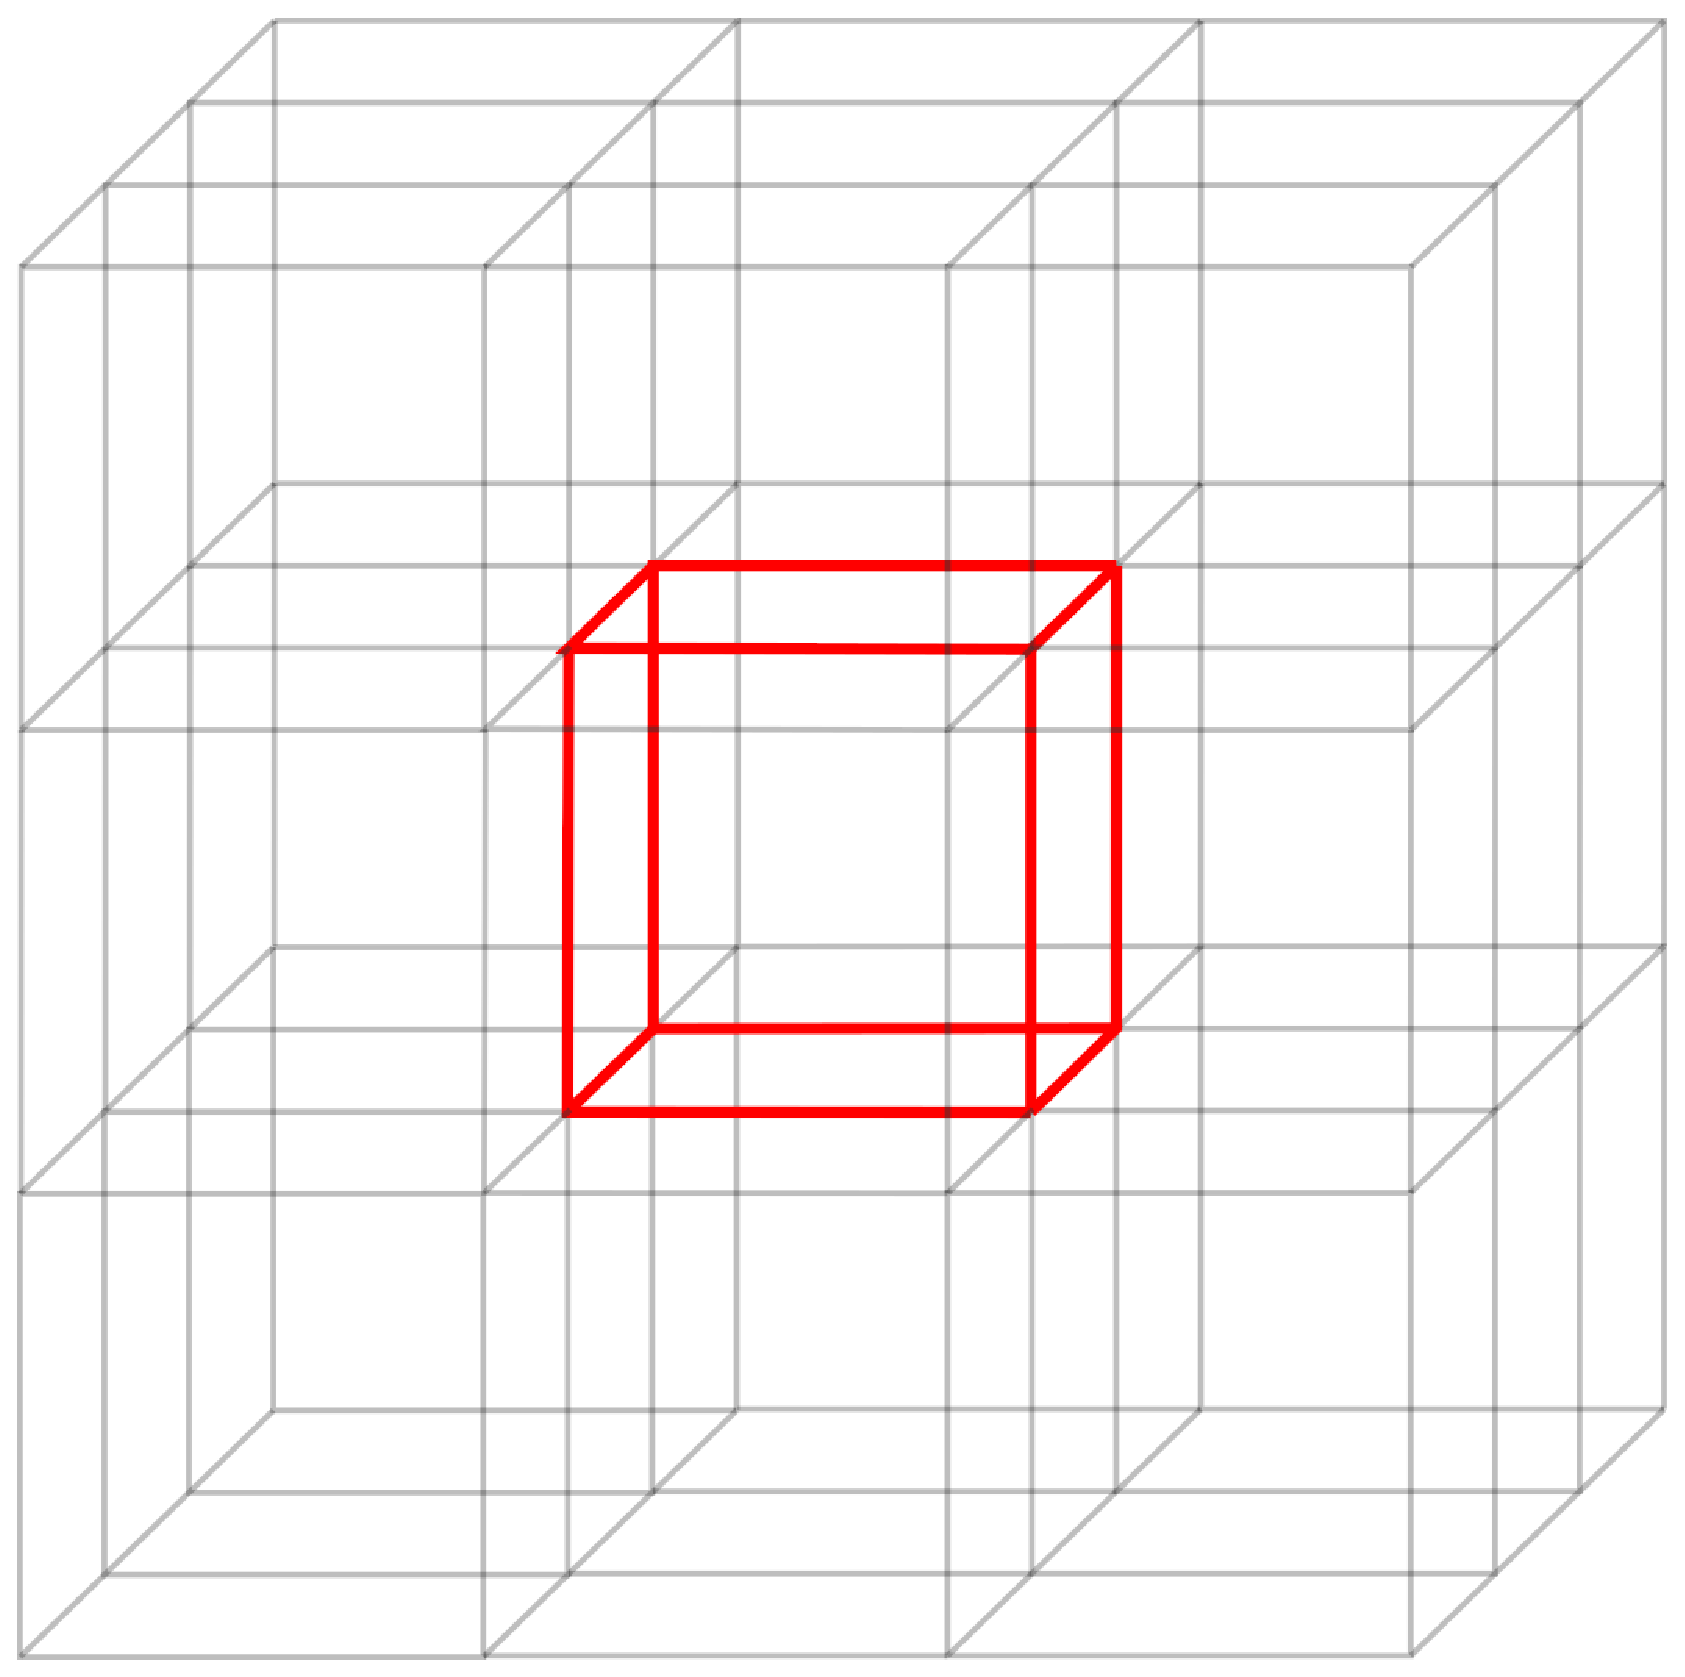
\includegraphics[width=\pwdi]{img/pixel-27-2.eps}\\
Self + 26 neighbors\\[0.5cm]
\end{center}
\item Pixel on the boundary of the pixel grid :\\
$p_{axis} = 0$ or $p_{axis} =  n_{p}(axis)-1$ \\
%\begin{blockarray}{cp{1cm}cp{1cm}c}
%Face of the pixel grid & & Edge of the pixel grid & & Corner of the pixel grid \\[0.25cm]
%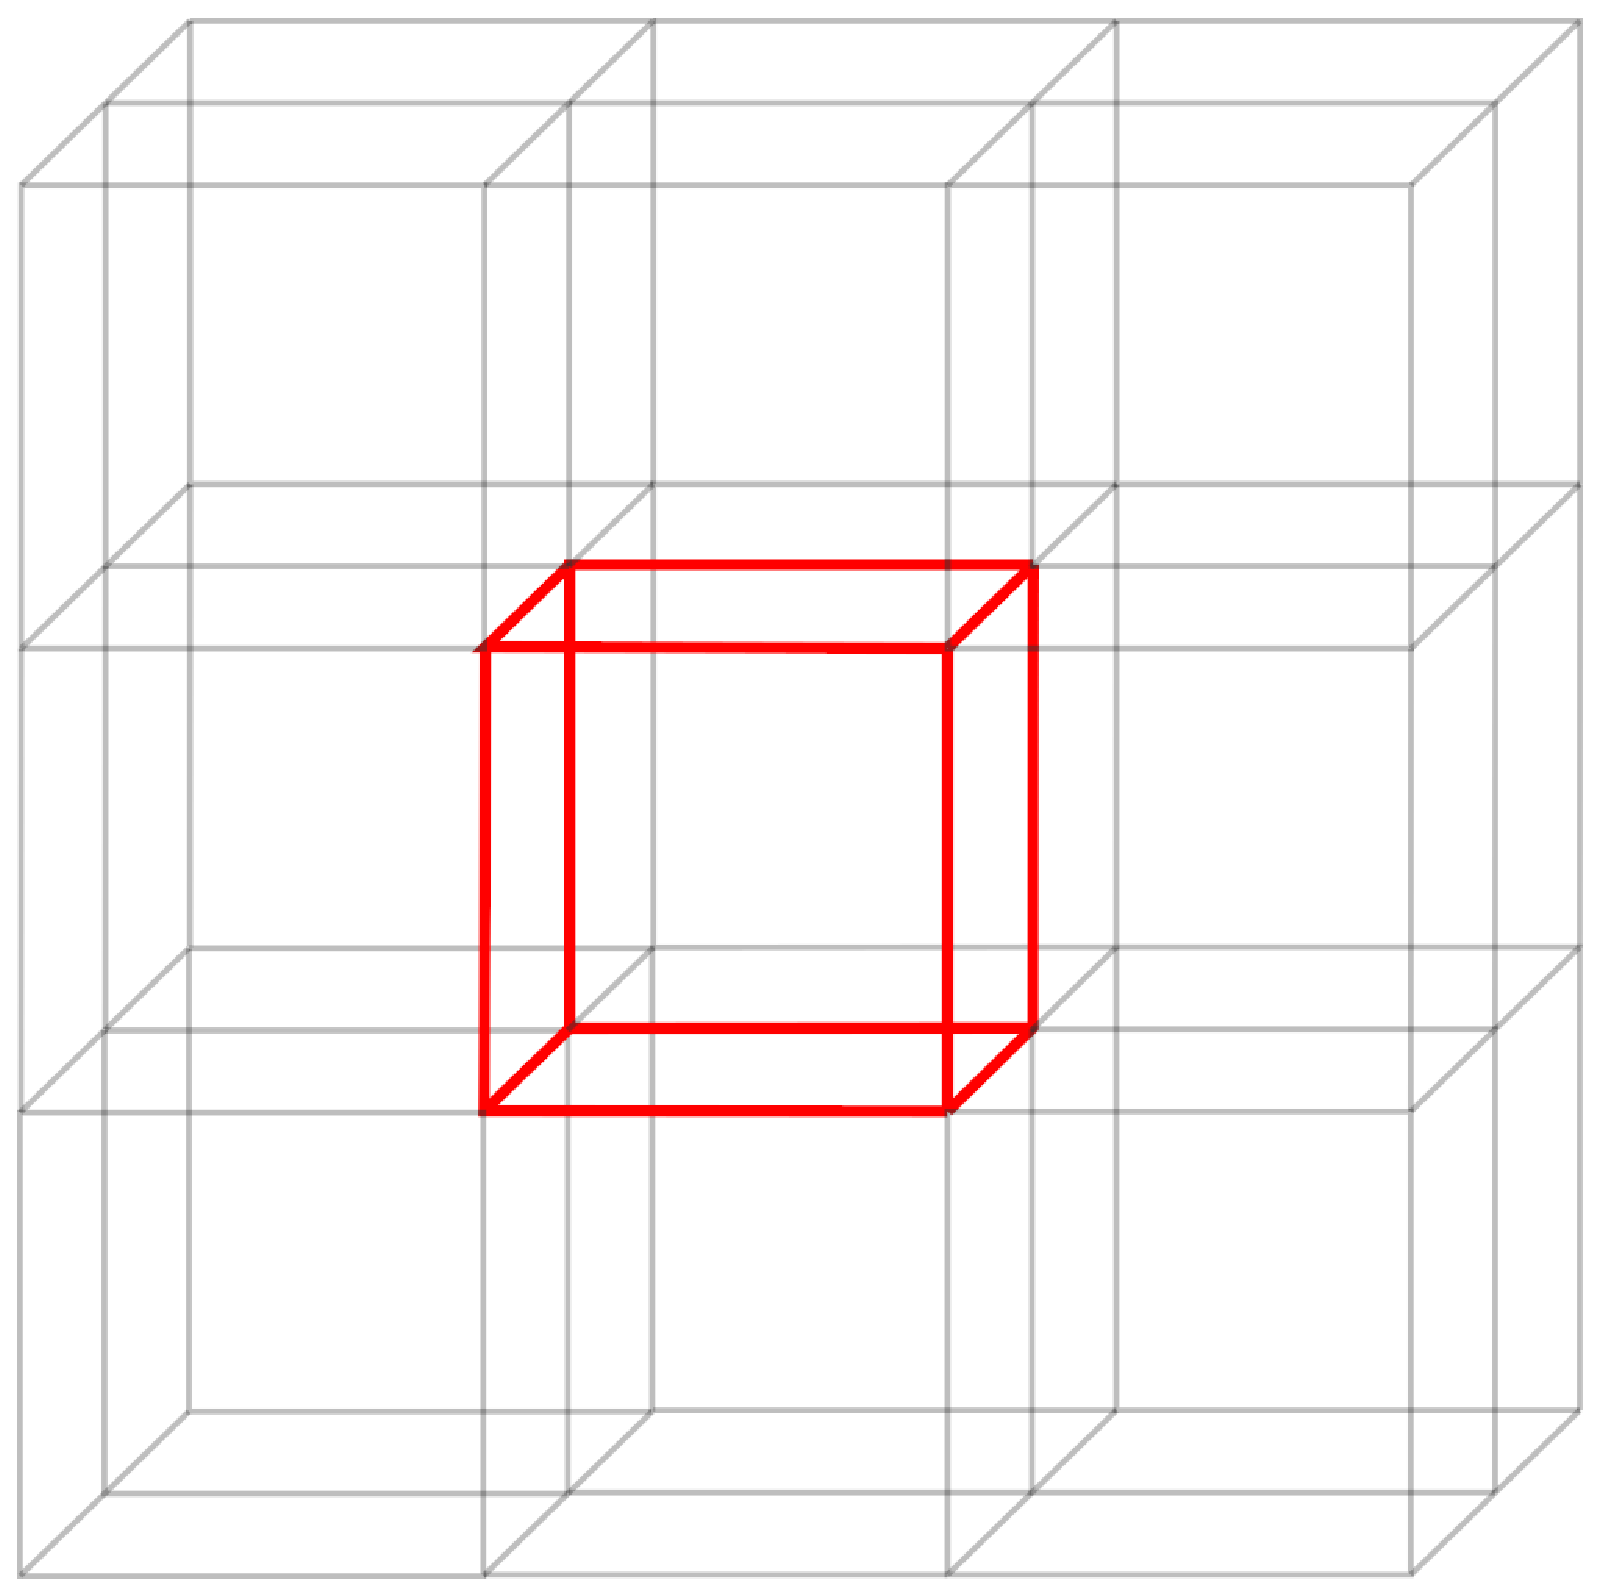
\includegraphics[width=3cm]{img/pixel-18-2.eps} & &
%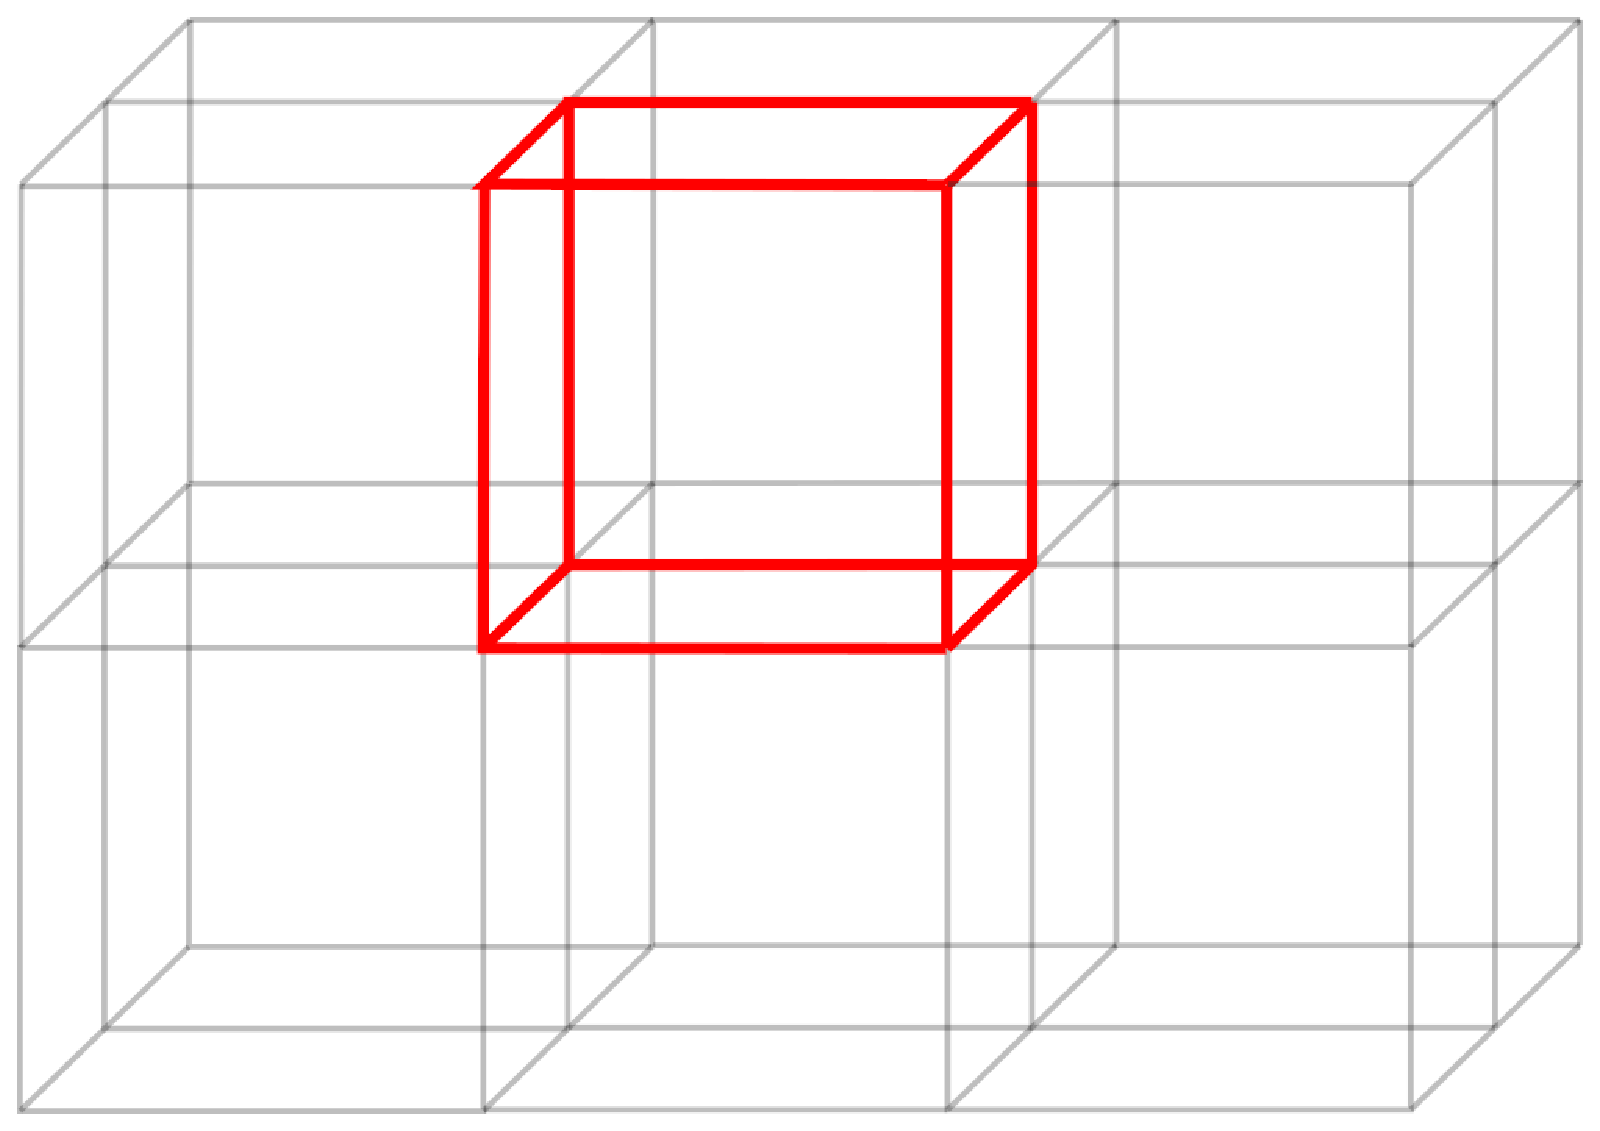
\includegraphics[width=3cm]{img/pixel-12-2.eps} & &
%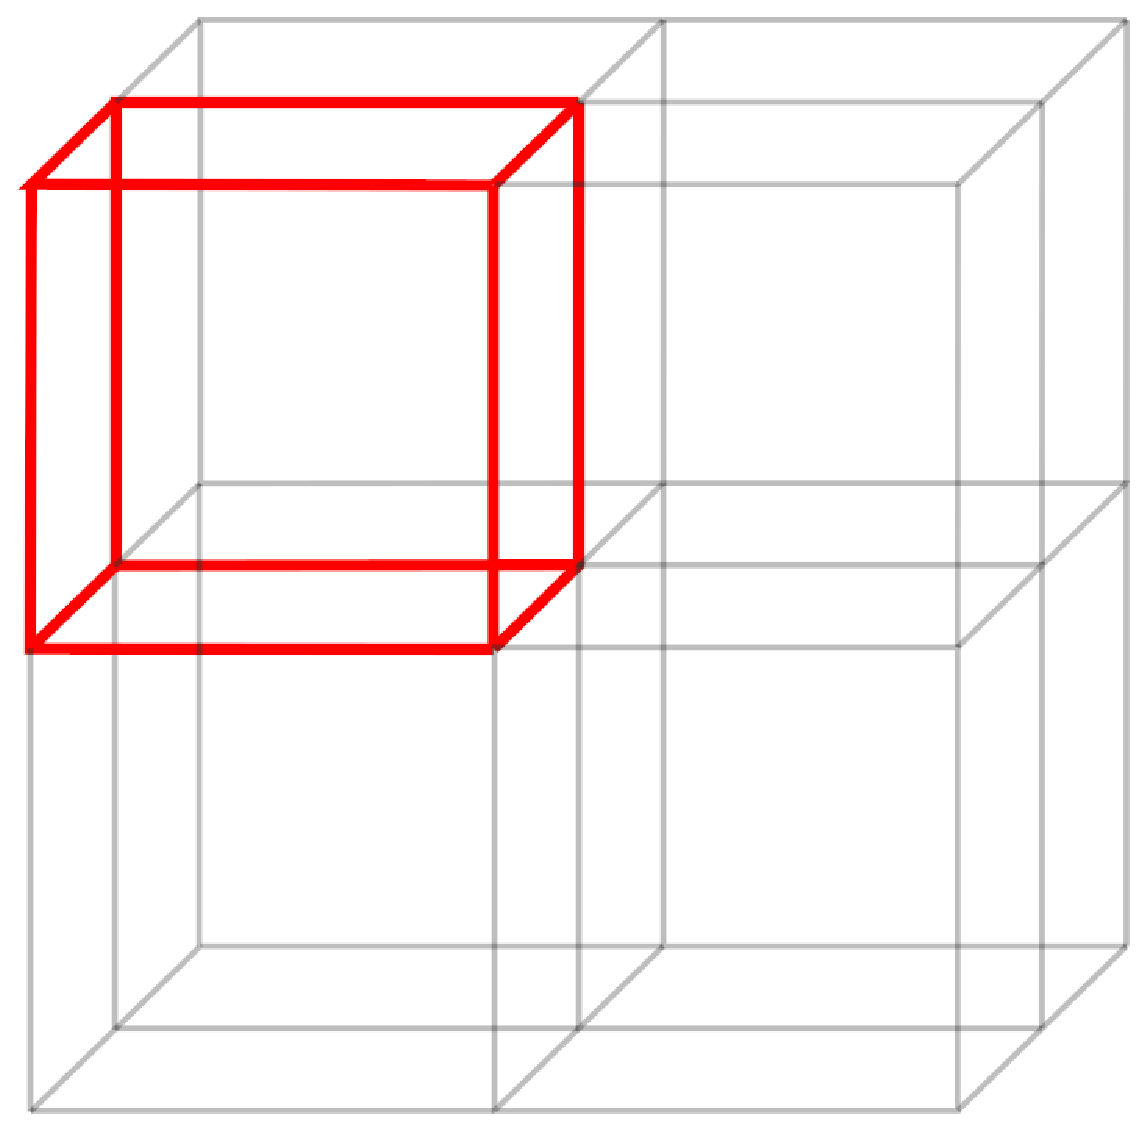
\includegraphics[width=2.175cm]{img/pixel-8-2.eps} \\
%Self + 17 neighbors & & Self + 11 neighbors & & Self + 7 neighbors \\
%\end{blockarray}
\begin{center}
Face of the pixel grid \\[0.25cm]
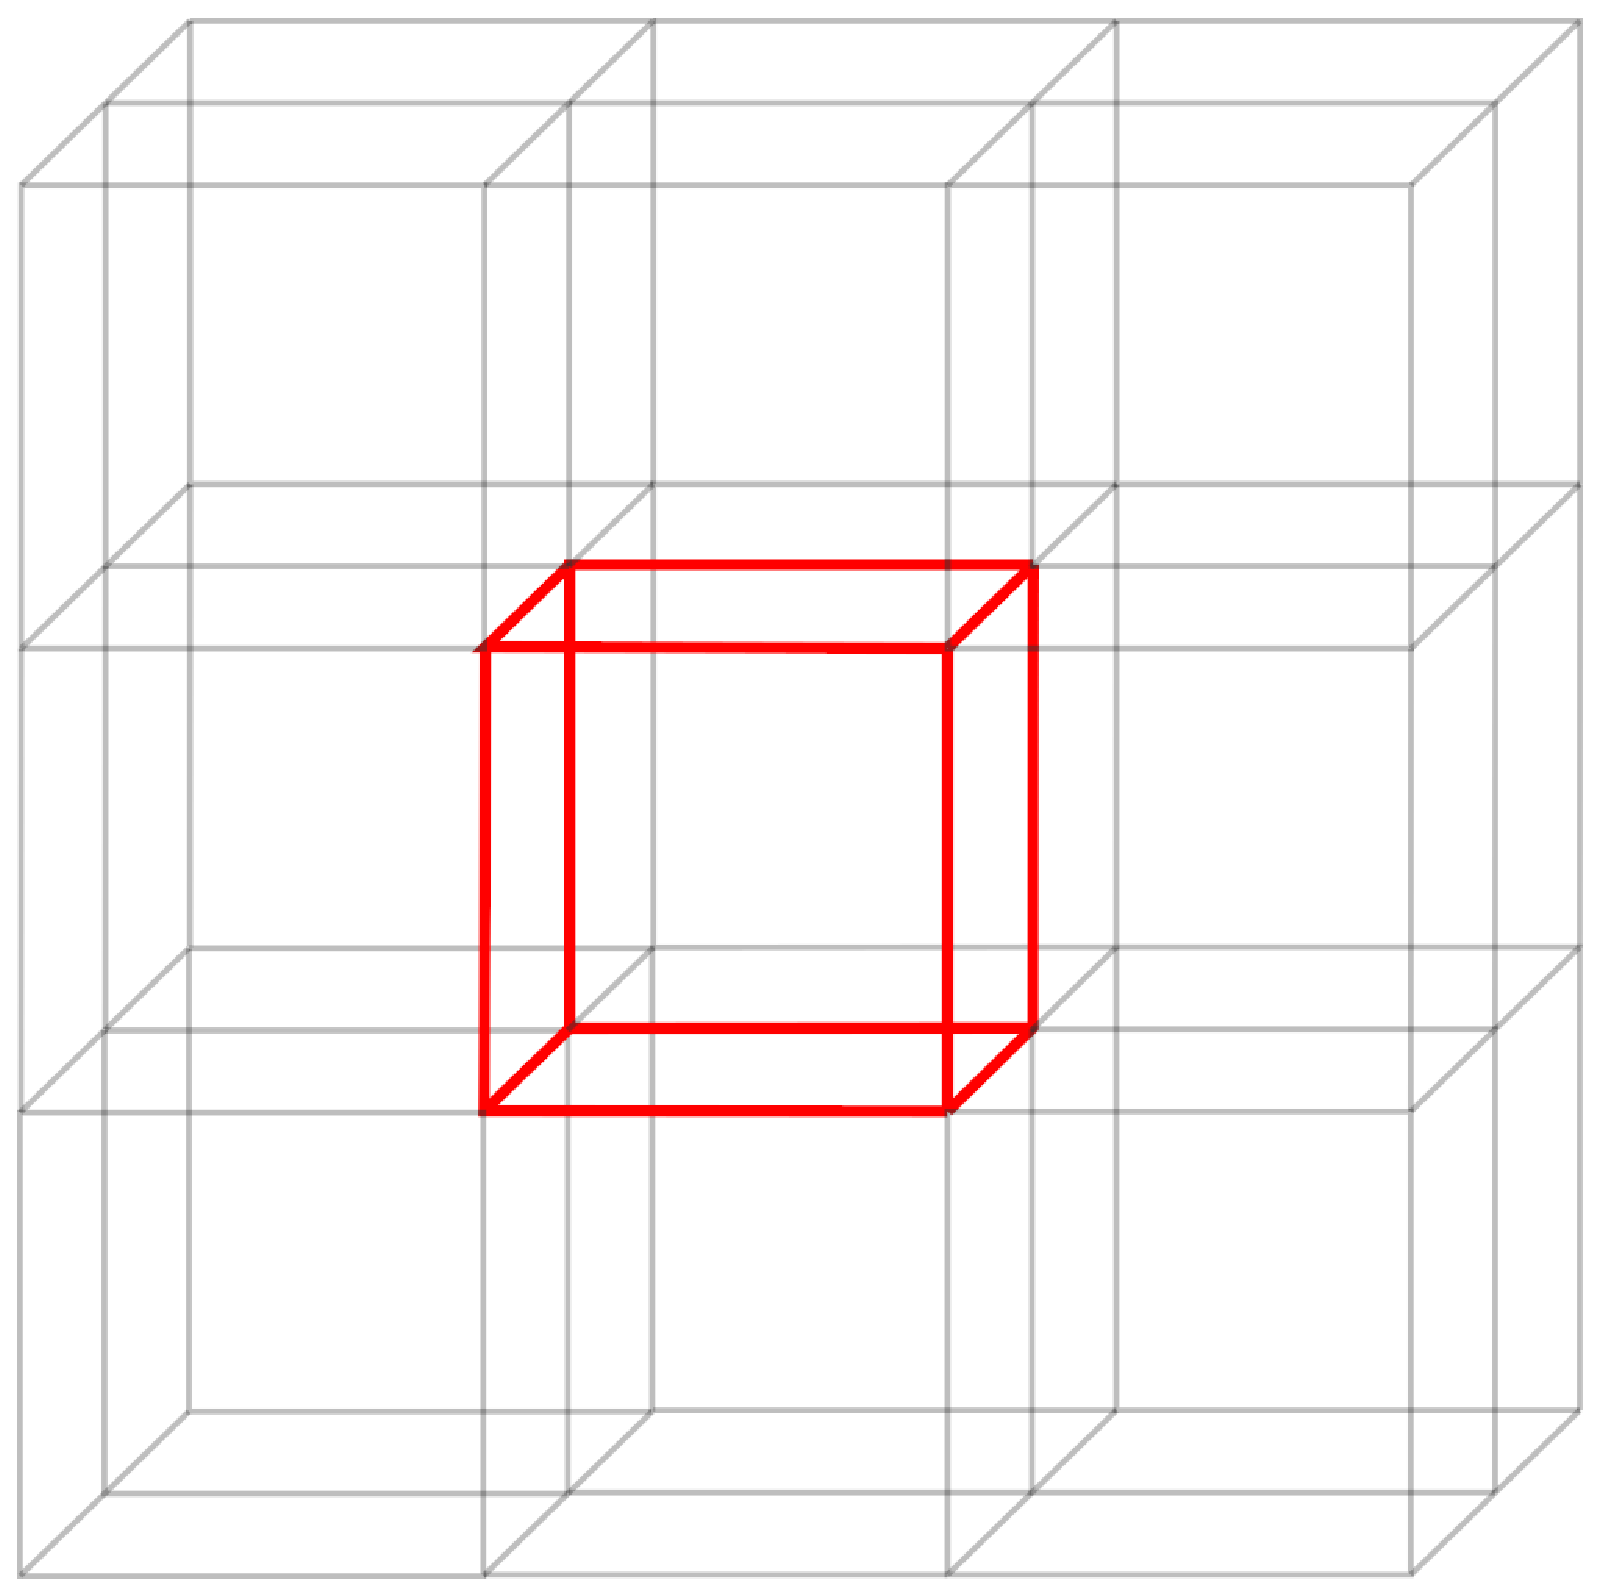
\includegraphics[width=\pwdi]{img/pixel-18-2.eps} \\
Self + 17 neighbors \\[0.5cm]
Edge of the pixel grid \\[0.25cm]
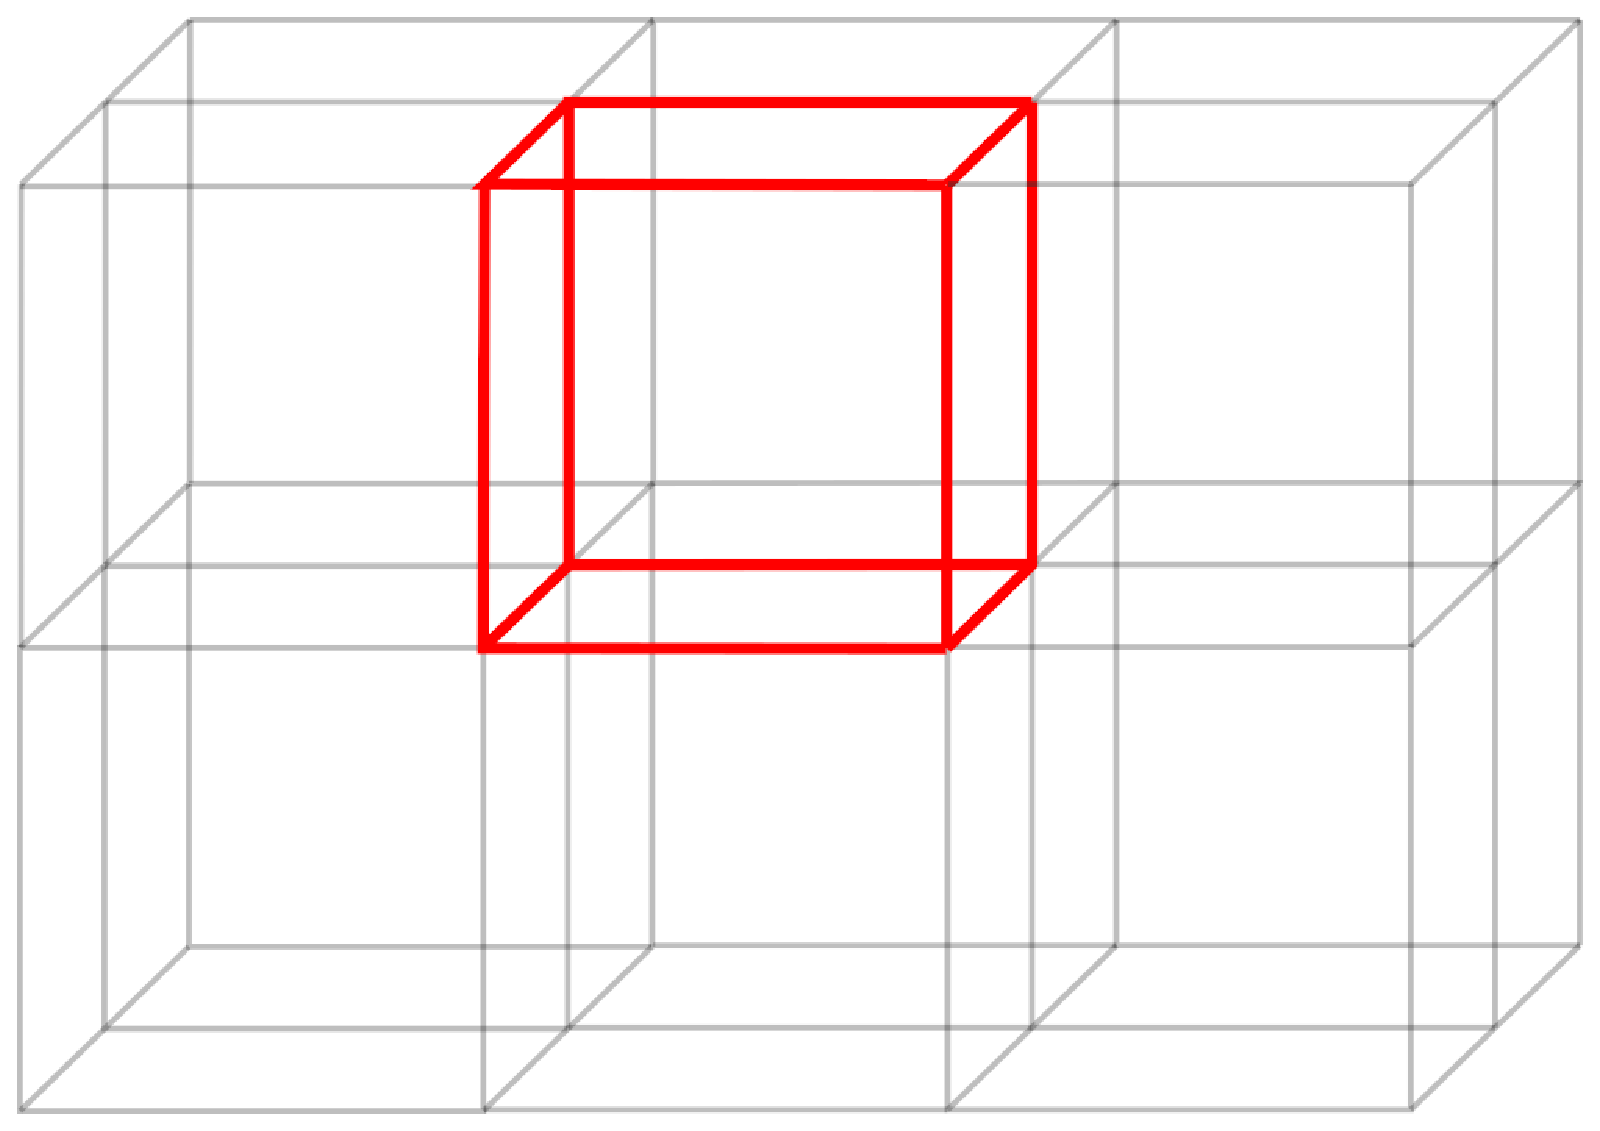
\includegraphics[width=\pwdi]{img/pixel-12-2.eps} \\
Self + 11 neighbors \\[0.5cm]
Corner of the pixel grid \\[0.25cm]
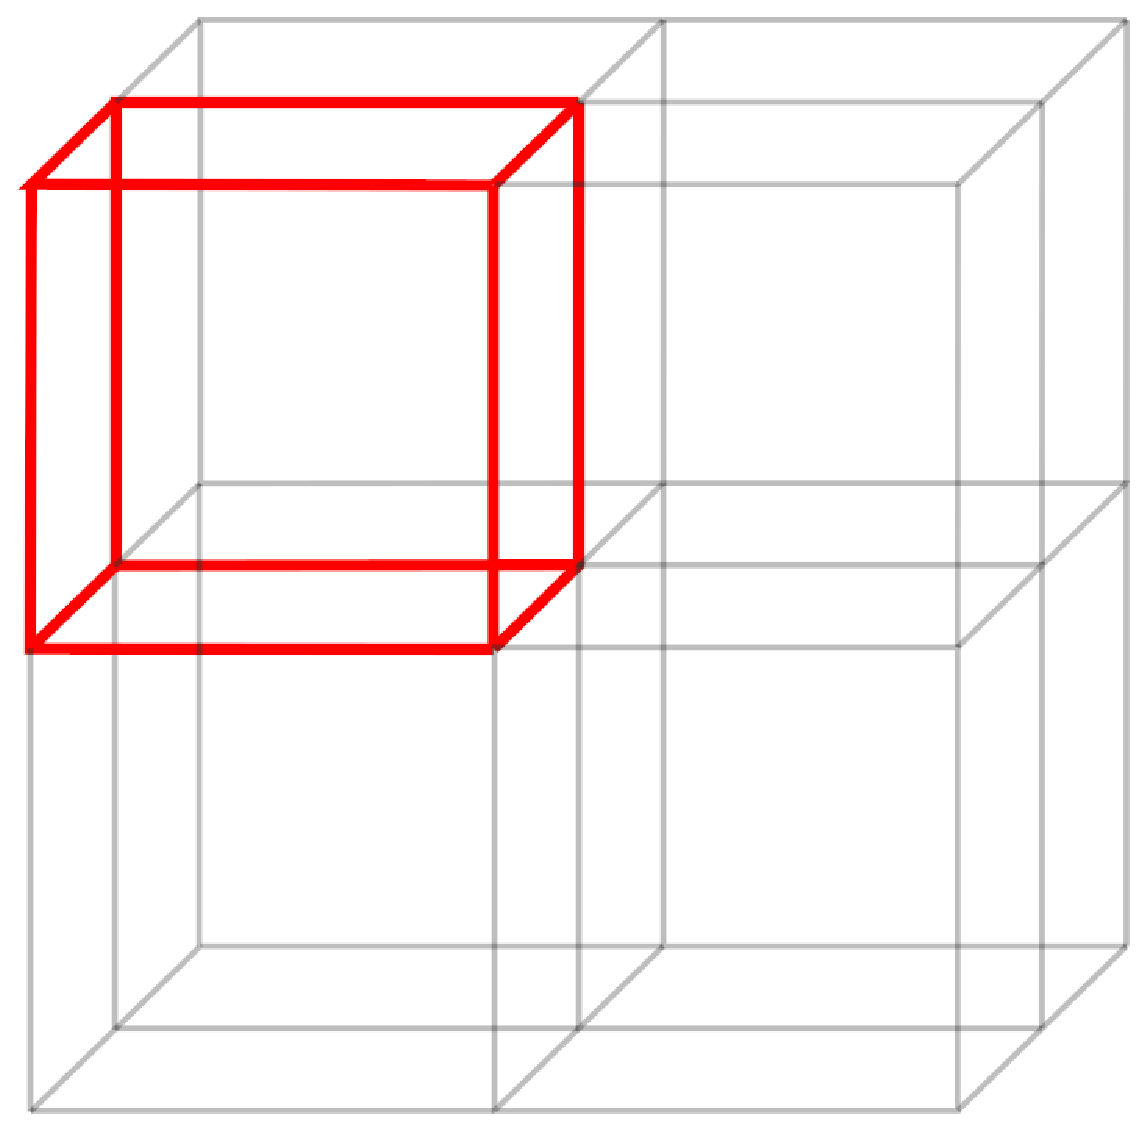
\includegraphics[width=\pwdj]{img/pixel-8-2.eps} \\
Self + 7 neighbors
\end{center}
\end{itemize}
Pixel neighbors are determined as illustrated in figure~\ref{pixelmap}: \\
\vspace{-1cm}
\begin{figure*}[!h]
\begin{center}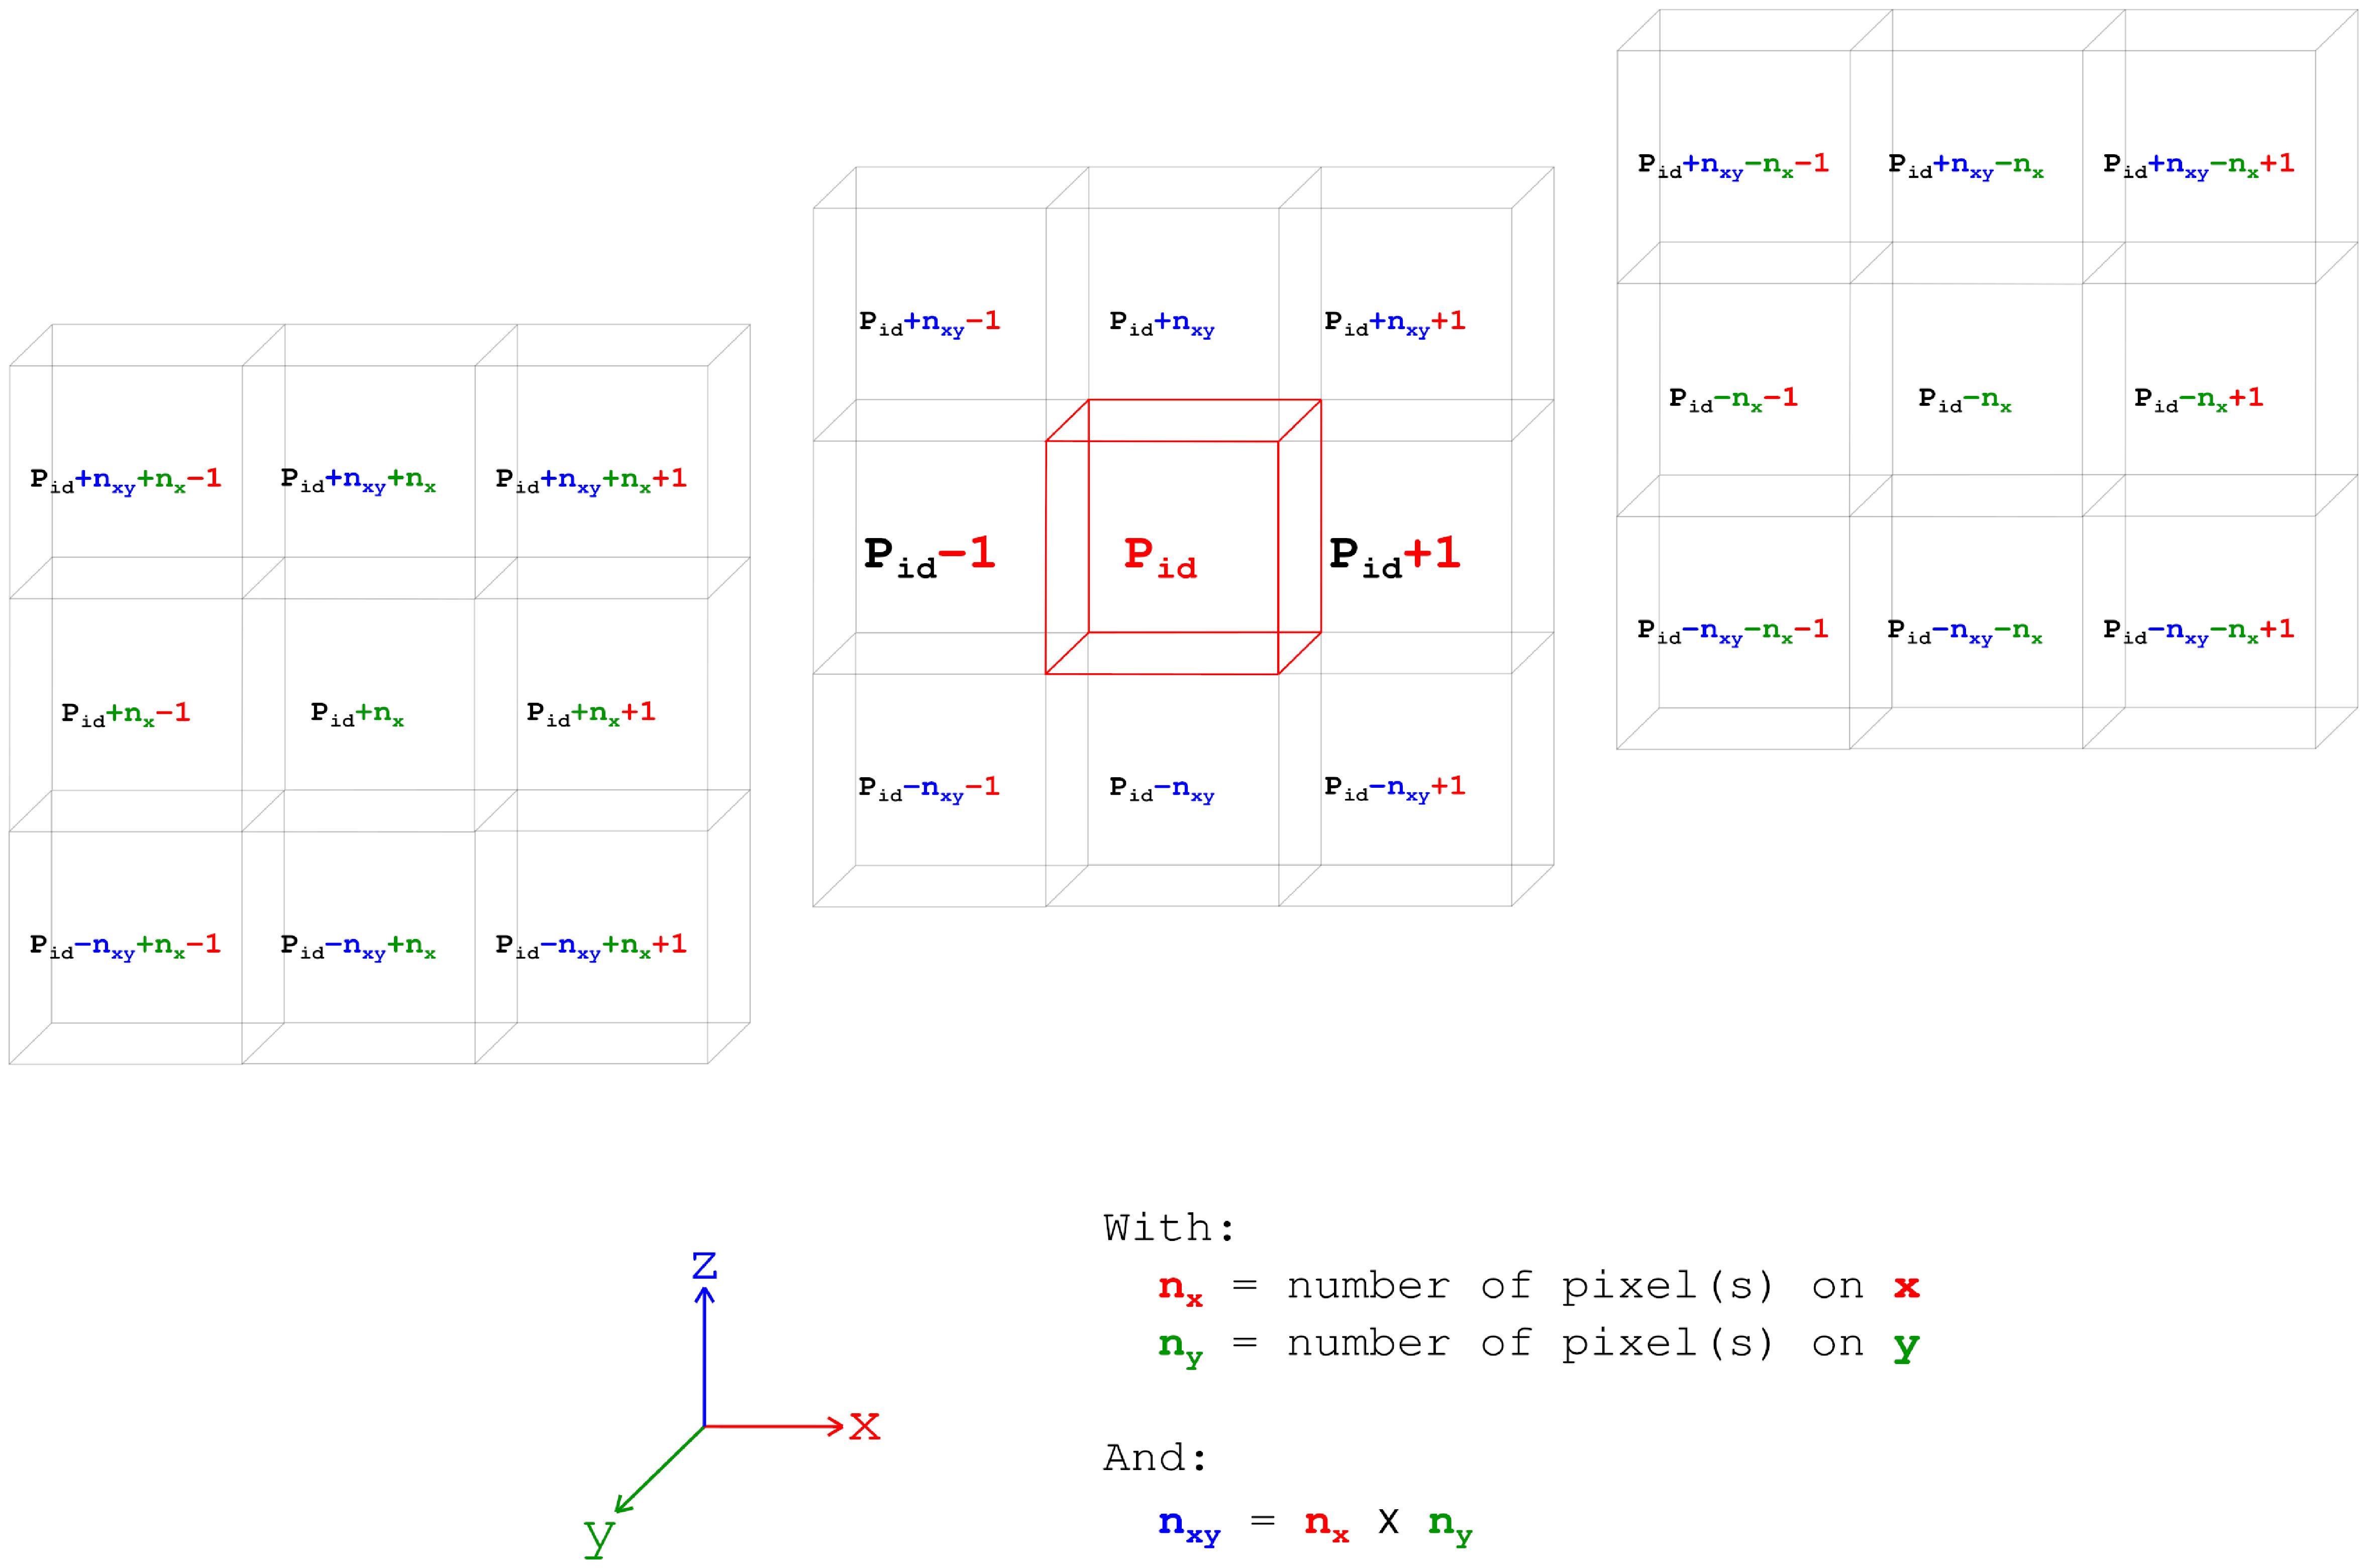
\includegraphics[width=15cm]{img/pix-map.eps}\end{center}
\caption{Finding pixel neighbors for pixel P$_{id}$: operation(s) on each axis are illustrated in the appropriate color(s)\label{pixelmap}}
\end{figure*}
\end{itemize}
\vspace{0.5cm}
Note that this kind of approach only makes sense if the number of pixels in the grid is high enough so that all pixels are not neighbors. 

\newpage
\subsection{With Periodic Boundary Conditions}

Non-cubic symmetries make it more complicated to offer a general methodology to deal with periodic systems:  
\begin{itemize}
\item[1.] Evaluate the number of pixel(s) on each axis, $n_{p}(x)$, $n_{p}(y)$ and $n_{p}(z)$, using equations \ref{e_npix} and \ref{e_dmax}. 
\item[2.] Convert atomic Cartesian coordinates to fractional coordinates using $\Tf$. \\
Using the transformation to fractional coordinates is the easiest way to compute the distance between atoms in the model.  
The problem requires to consider the periodicity of the system, and, in the case of non-cubic symmetry transformations, could be tricky when using Cartesian coordinates. 
Working with fractional coordinates is much easier since in that case corrections are performed simply adding or subtracting multiples of 1.0 on any fractional direction.
\begin{itemize}
\item Convert Cartesian coordinates to fractional coordinates ($f_{x}$, $f_{y}$, $f_{z}$) using Eq.~\ref{c2f}. 
\item Compute corrected fractional coordinates ($f_{c,x}$, $f_{c,y}$, $f_{c,z}$) inside the model box:
\begin{equation}
f_{c,axis} = f_{axis} - \left\lfloor f_{axis} \right\rfloor \qquad \textrm{with}\qquad 0 \le f_{c,axis} < 1
\end{equation}
\end{itemize}
\item[3.] Pixel positions ($p_x$, $p_y$, $p_z$) are determined using the atom's corrected fractional coordinates ($f_{c,x}$, $f_{c,y}$, $f_{c,z}$):
\begin{equation}
p_{axis} = \left\lfloor f_{c,axis} \times n_{p}(axis) \right\rfloor \qquad \textrm{with} \qquad p_{axis} \in [0, n_{p}(axis)-1]
\end{equation}
\item[4.] Determine each pixel neighbors: 
\begin{itemize}
\item Pixel inside the pixel grid:
\begin{center}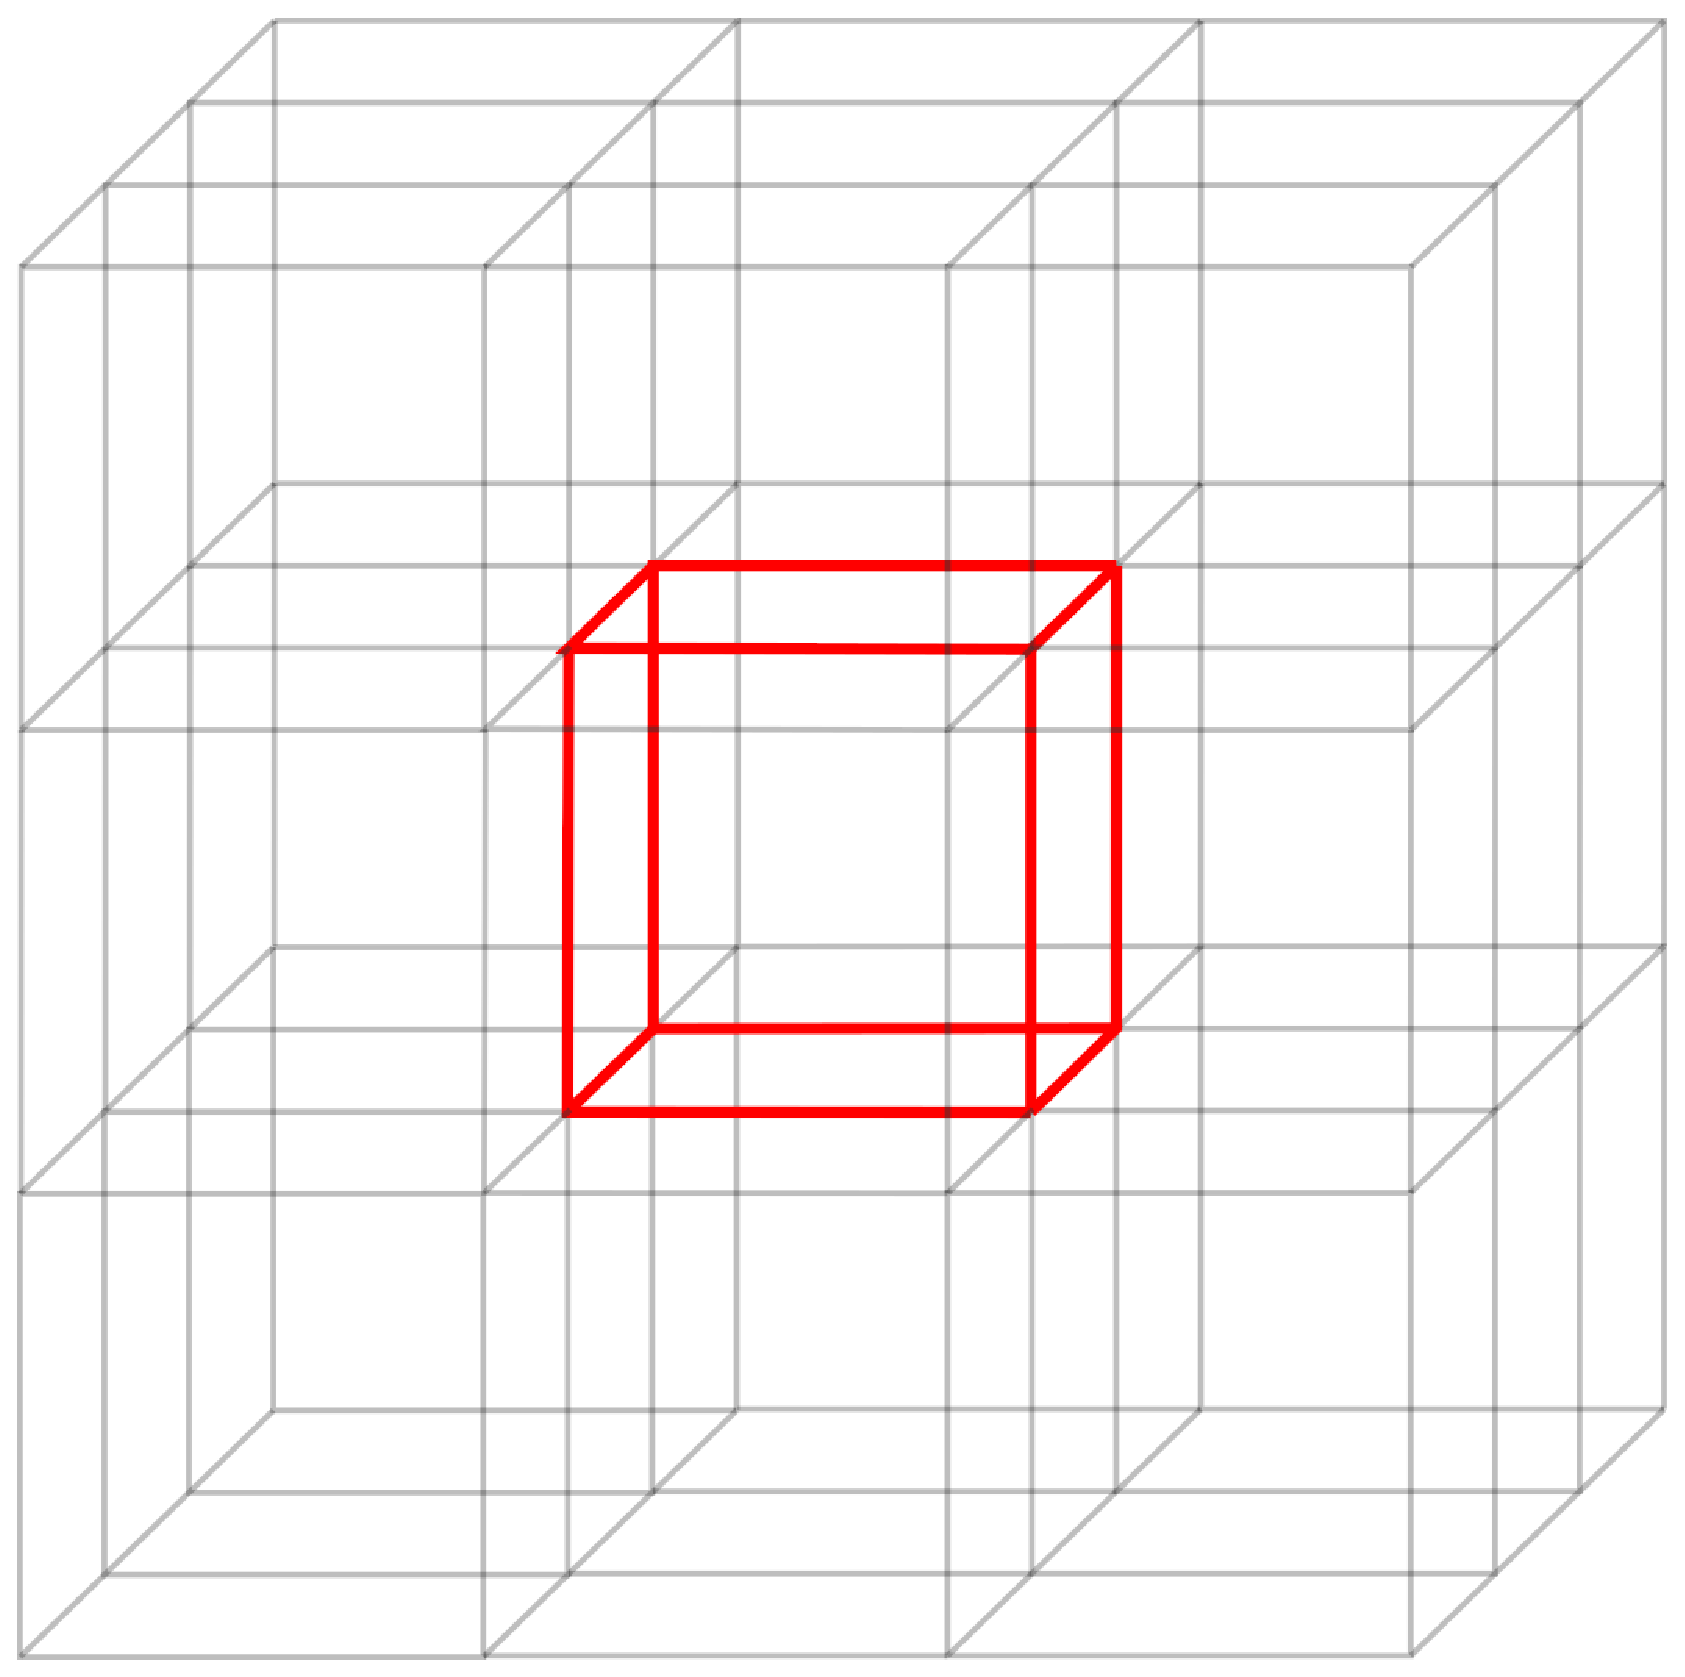
\includegraphics[width=4cm]{img/pixel-27-2.eps} \\[0.25cm]
Self + 26 neighbors, no PBC transformation required. 
\end{center}
\clearpage
\item Pixel on the boundary of the pixel grid :\\
$p_{axis} = 0$ or $p_{axis} =  n_{p}(axis)-1$ \\ 
\begin{center}
Face of the pixel grid: \\[0.25cm] 
\begin{blockarray}{ccc}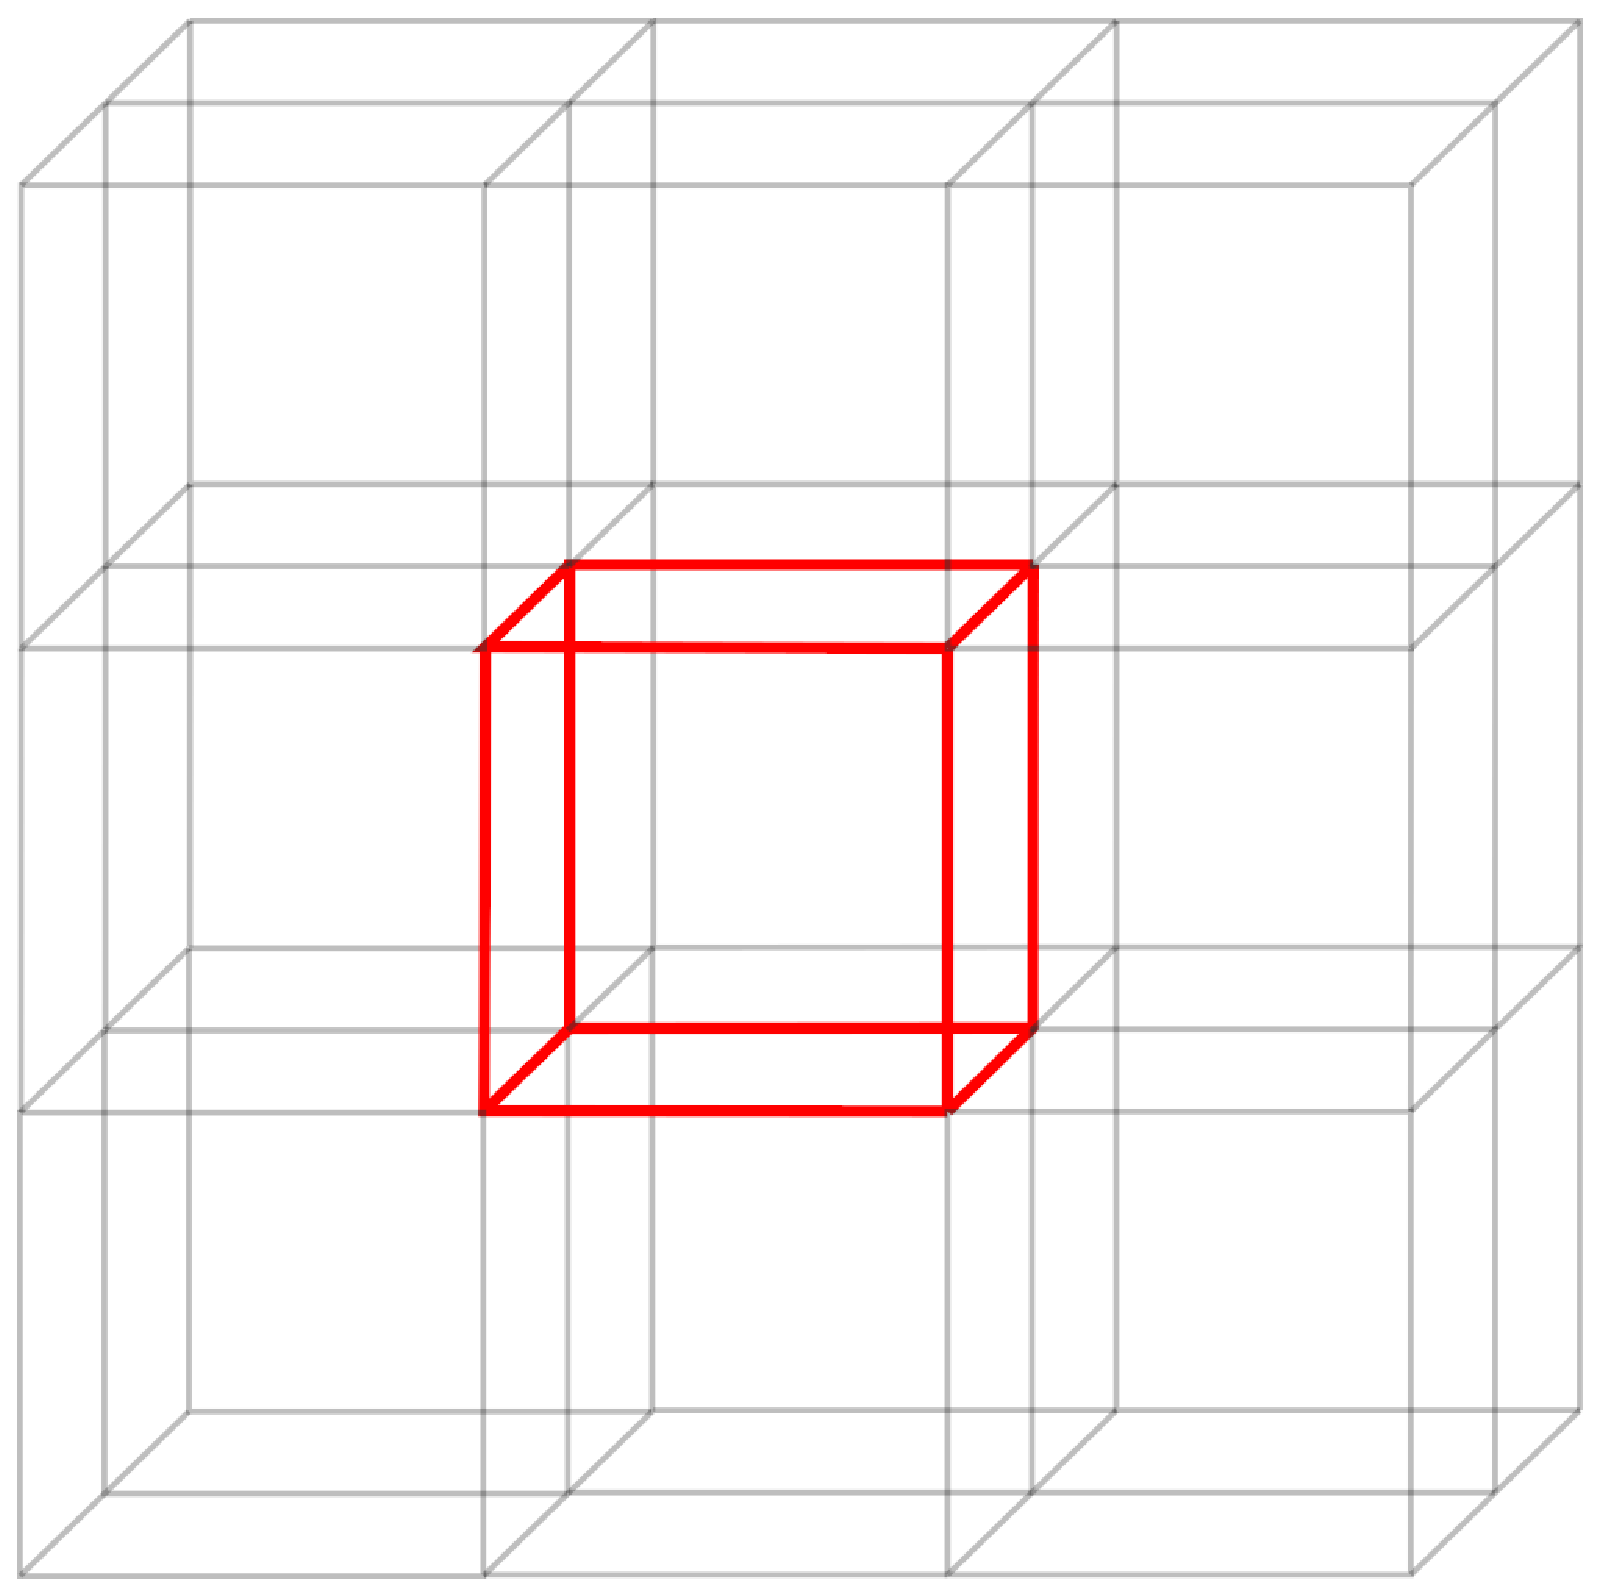
\includegraphics[width=\pwdi]{img/pixel-18-2.eps} & \raisebox{\rsv}{+} & 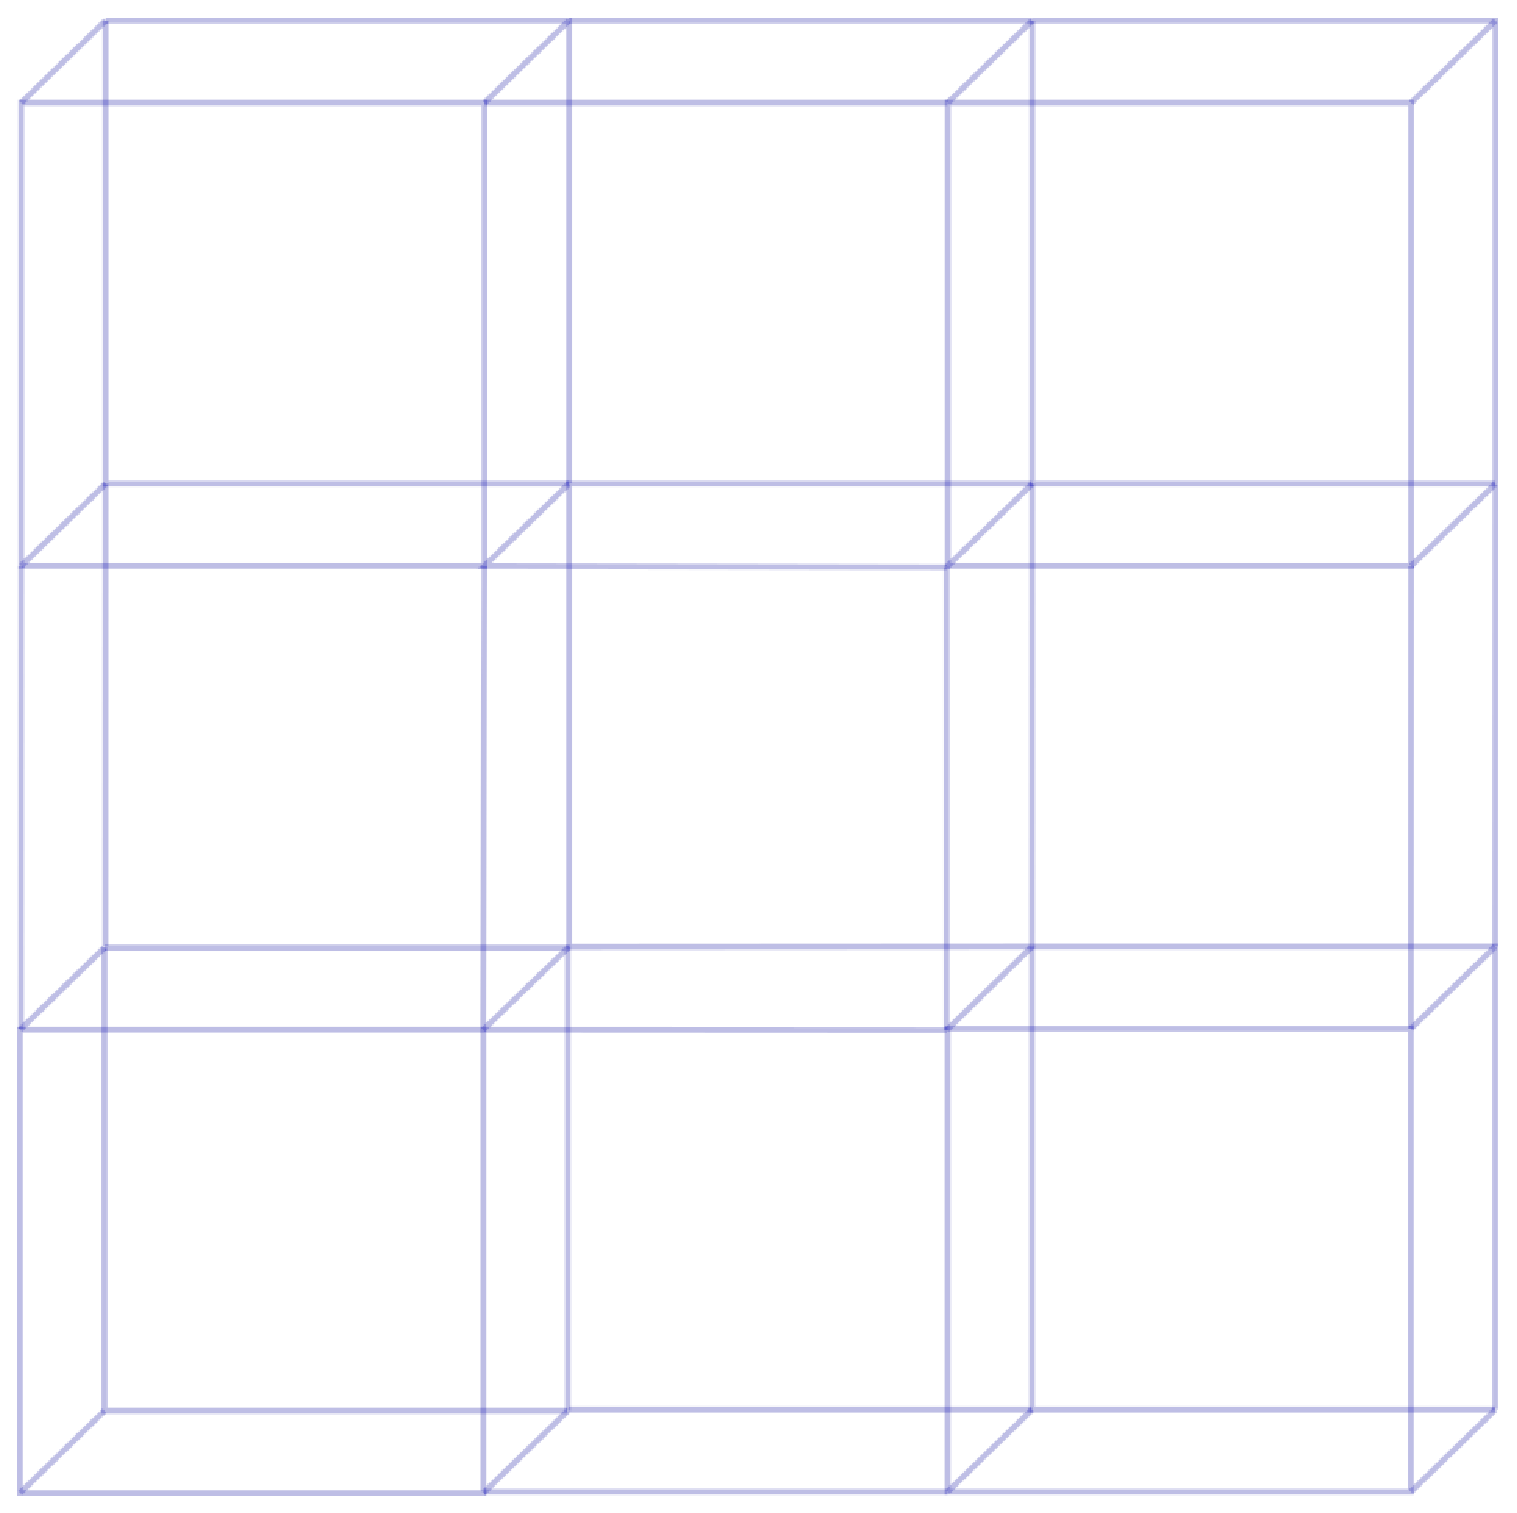
\includegraphics[width=\pwdi]{img/pixel-18-9.eps} \end{blockarray} \\
Self + 17 + 9 neighbors using PBC \\[0.5cm]
Edge of the pixel grid: \\[0.25cm]
\begin{blockarray}{ccc}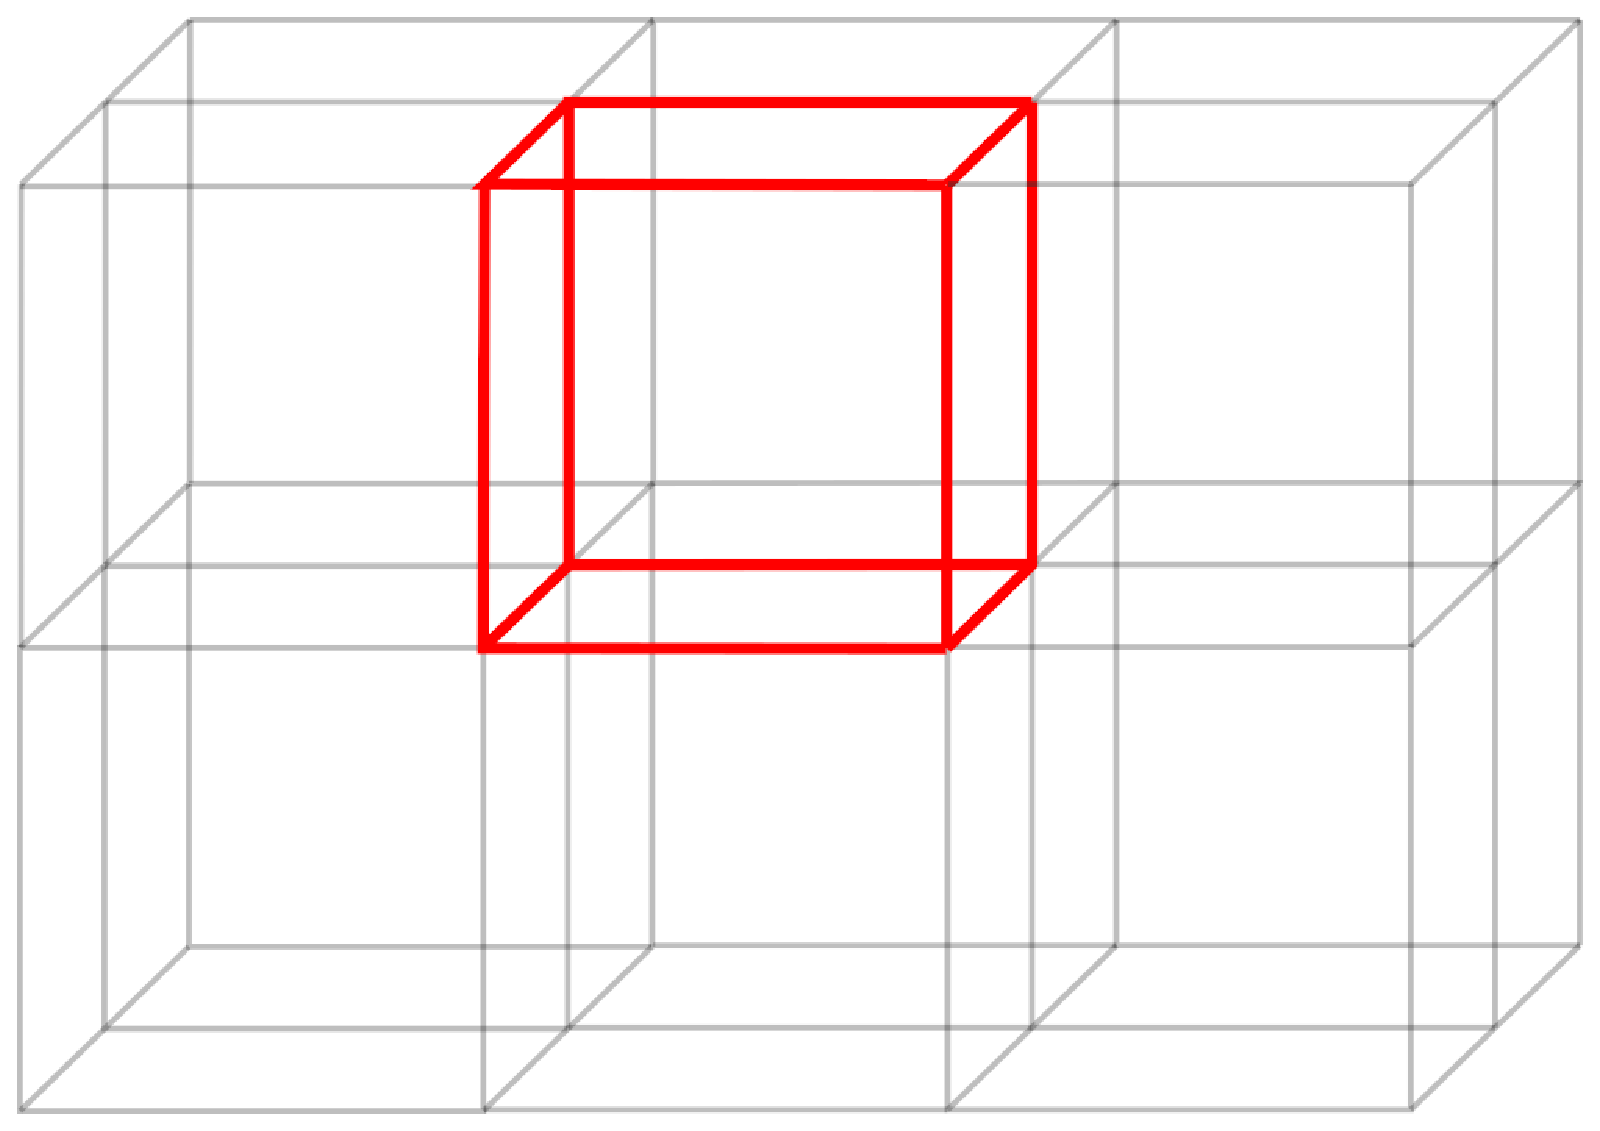
\includegraphics[width=\pwdi]{img/pixel-12-2.eps} & \raisebox{\rsv}{+} & 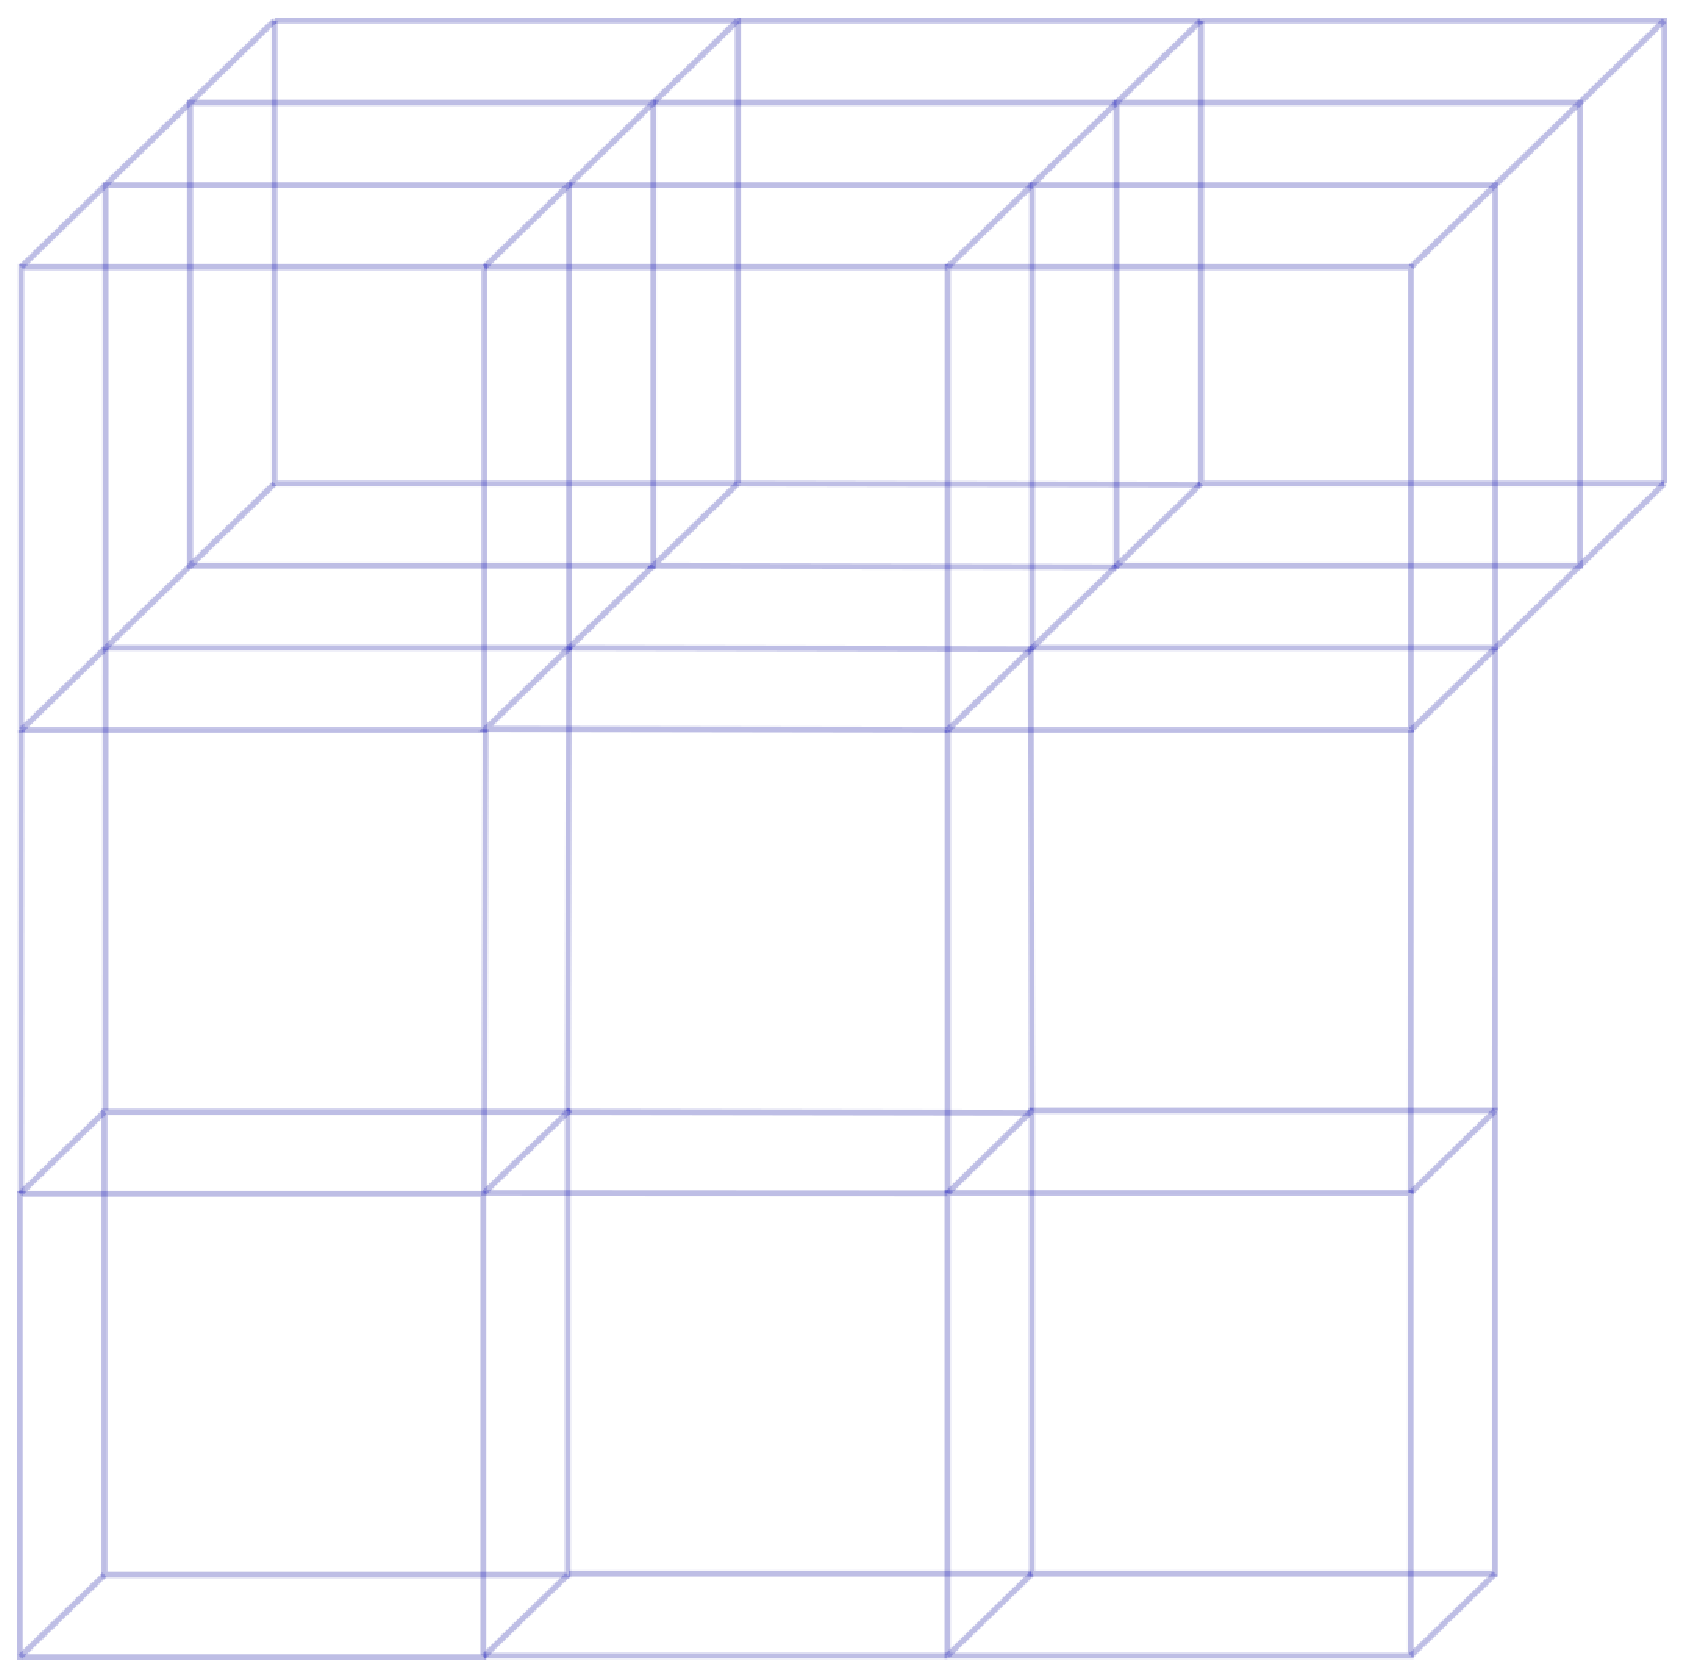
\includegraphics[width=\pwdi]{img/pixel-12-15.eps} \end{blockarray} \\
Self + 11 + 15 neighbors using PBC \\[0.5cm]
Corner of the pixel grid: \\[0.25cm]
\begin{blockarray}{ccc}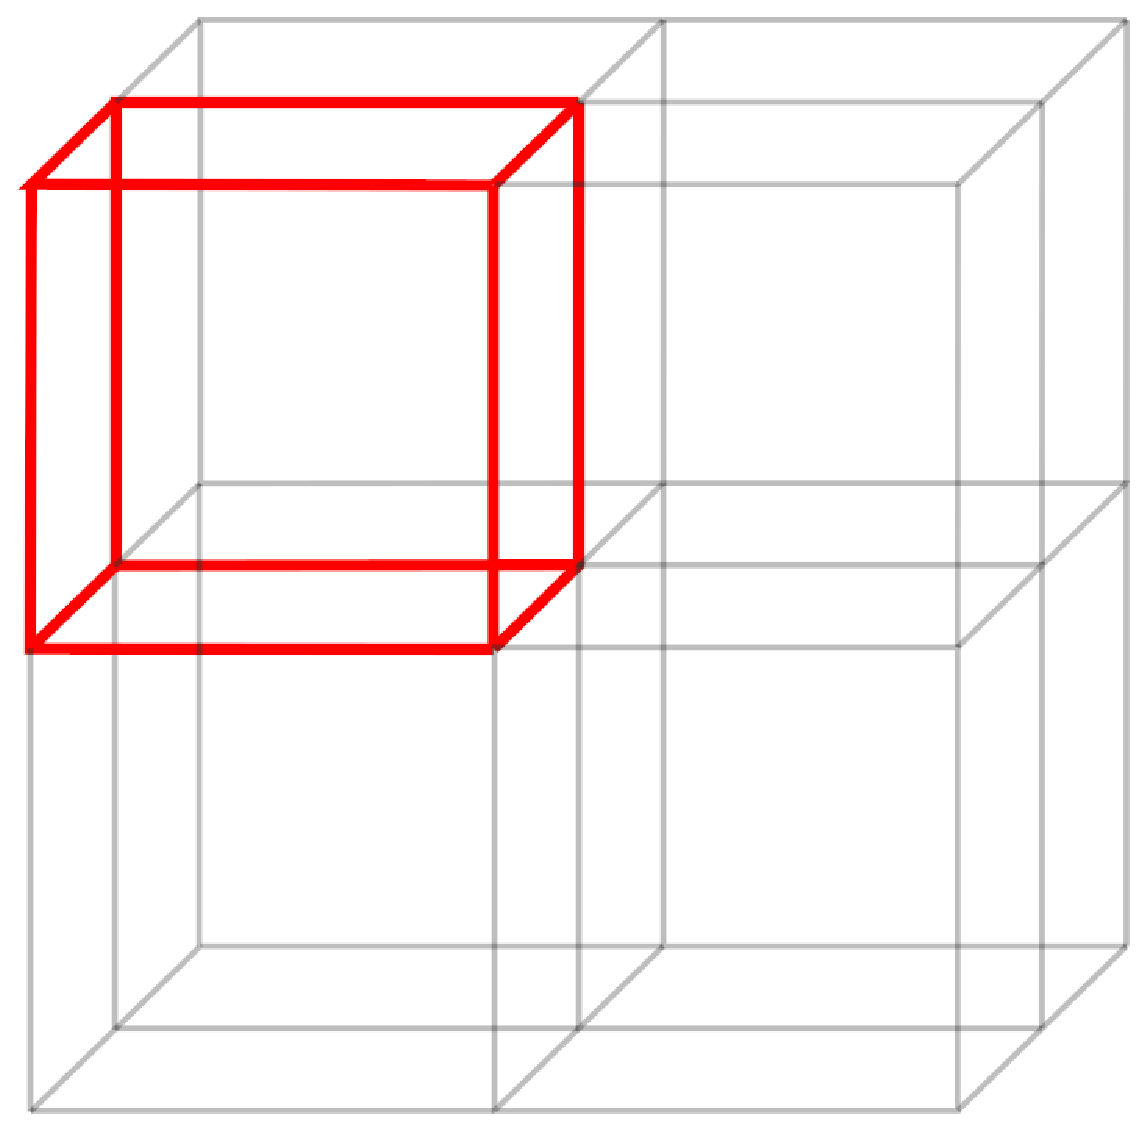
\includegraphics[width=\pwdj]{img/pixel-8-2.eps} & \raisebox{\rsv}{+} & 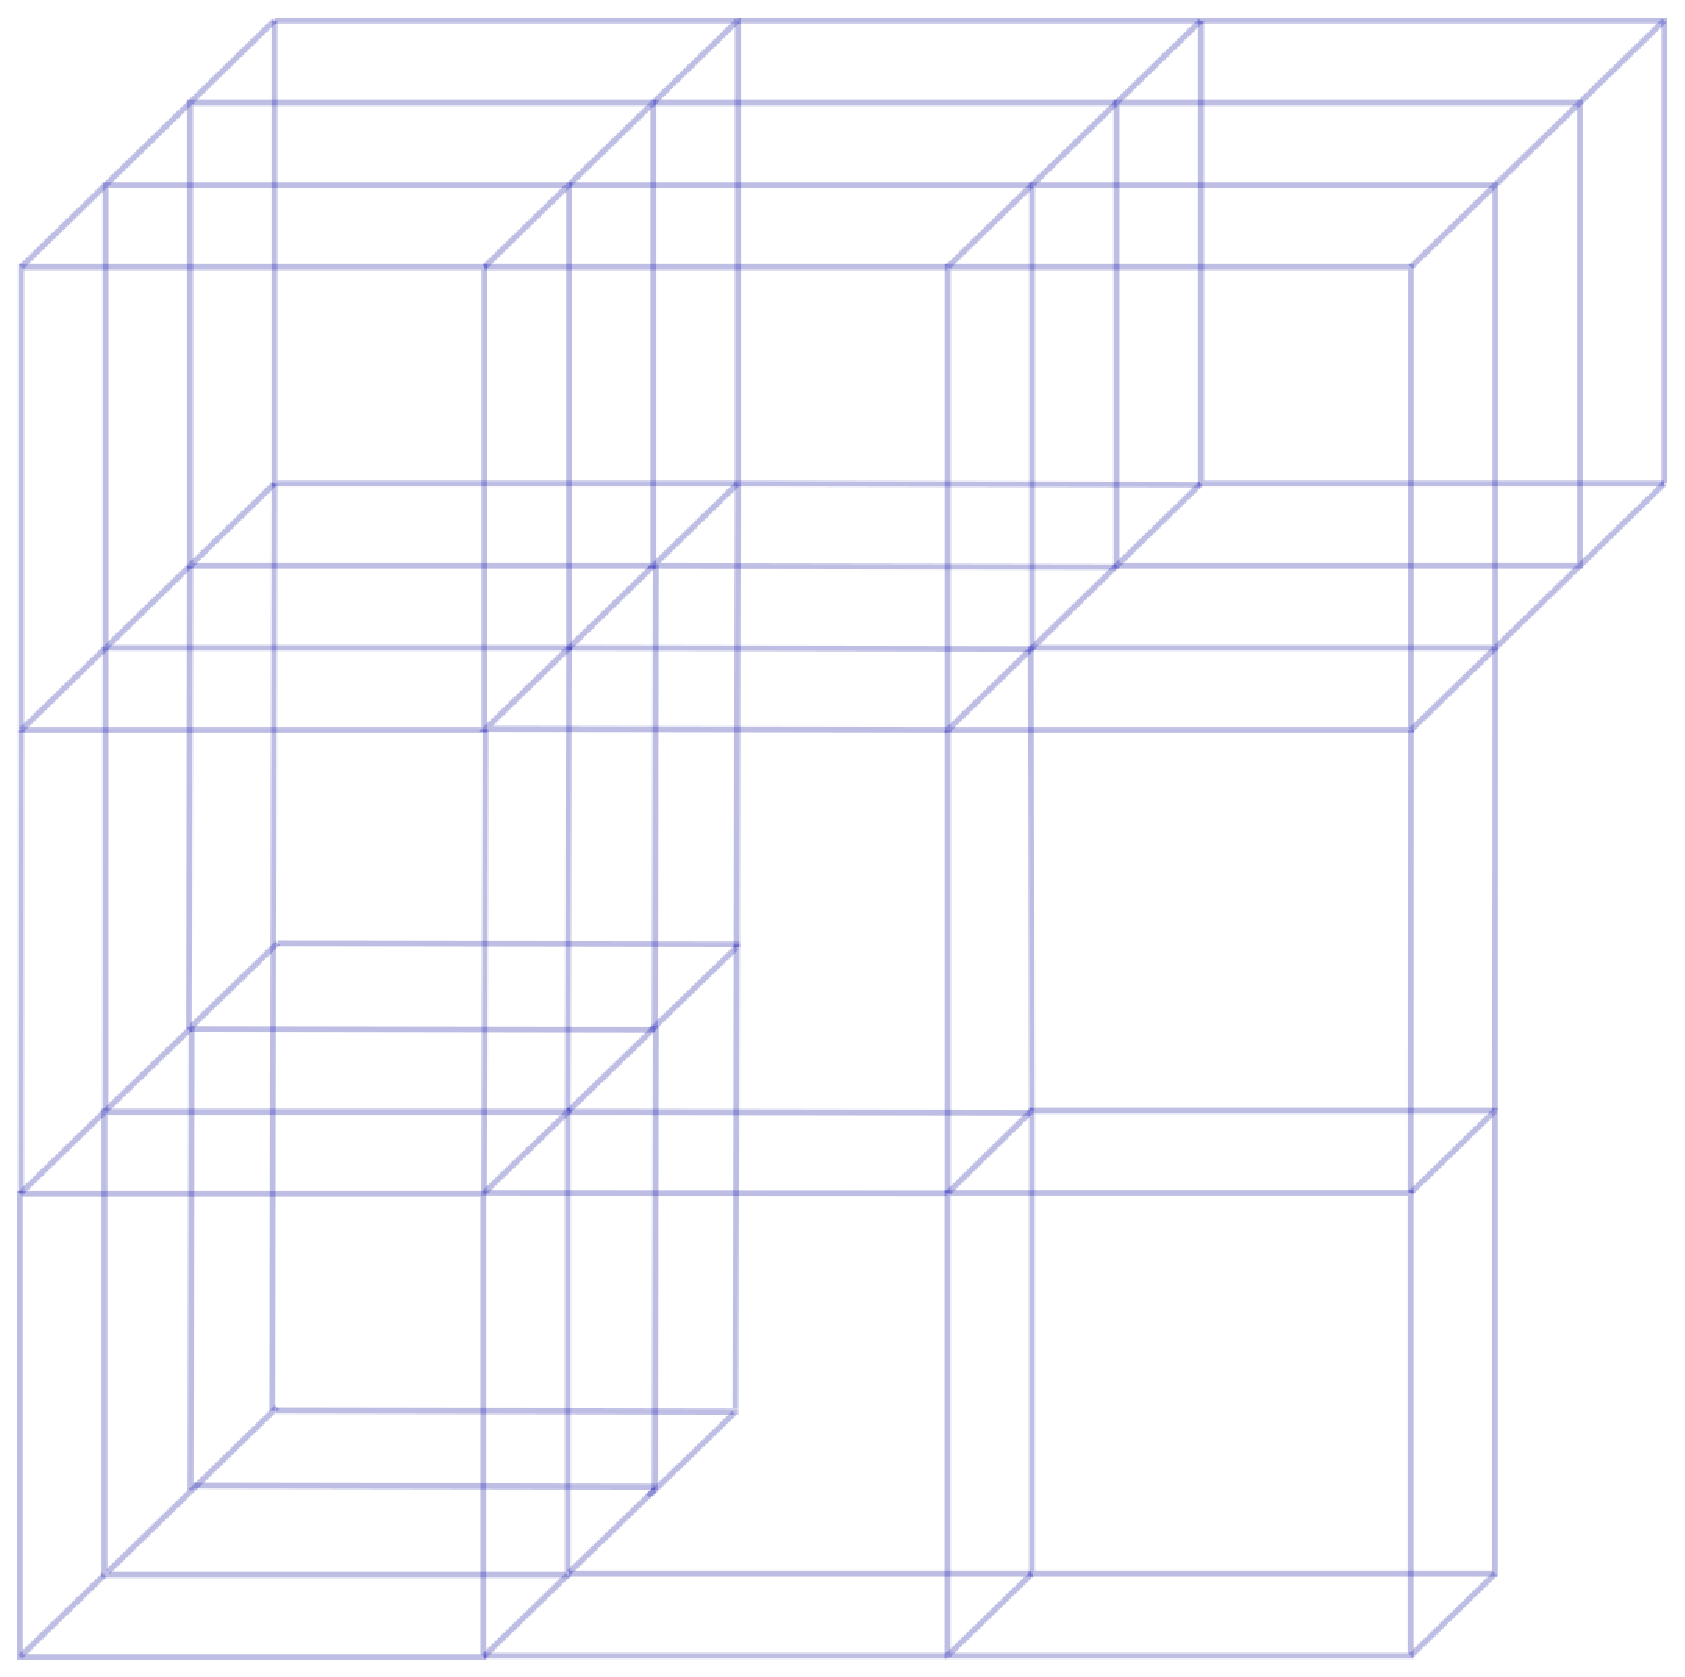
\includegraphics[width=\pwdi]{img/pixel-8-19.eps} \end{blockarray} \\
Self + 7 + 19 neighbors using PBC \\[0.5cm]
\end{center}
For a pixel with number $p_{id}$ with pixel coordinates ($p_x$, $p_y$, $p_z$) inside the pixel grid, pixel neighbors are determined as illustrated in figure~\ref{pixelmap}. 
For pixel on the boundary of the grid, then adjustments are required to find the neighbors via PBC. 
\end{itemize}
\clearpage
\item[5.] Compute the interatomic distance $D_{ab}$ between 2 atoms $a$ and $b$ using corrected fractional coordinates:
\begin{eqnarray}
f_{c,axis}(ab) & = & f_{c,axis}(a) - f_{c,axis}(b) \\[0.125cm]
f_{axis}(ab) & = & f_{c,axis(ab)} - \left\lfloor f_{c,axis(ab)} \right\rceil \\[0.125cm]
\vec{r}(ab) & = & \Tc \times \vec{f}(ab) \\[0.125cm]
\quad {\textrm{with}} \quad \vec{r}(ab) & = & \left( \begin{blockarray}{c}
r_x(ab) \\
r_y(ab) \\
r_z(ab)
\end{blockarray} \right) \\[0.125cm]
\quad {\textrm{and}} \quad \vec{f}(ab) & = & \left( \begin{blockarray}{c}
f_{x}(ab) \\
f_{y}(ab) \\
f_{z}(ab)
\end{blockarray} \right) \\[0.125cm]
D(ab) & = & \lvert \vec{r}(ab) \rvert
\end{eqnarray}
As mentioned in the previous section this approach only makes sense when the number of pixels in the grid is high enough so that all pixels are not neighbors. 
In the case where PBC are applied this means that the number of pixels on one dimension, $x$, $y$, or $z$ should be higher than 3. 
\end{itemize}
Commented codes that illustrate the entire work procedure are provided in: 
\begin{itemize}
\item C codes: \ref{c-pc-data} through \ref{c-pc-pixel}.
\item FORTRAN90 codes: \ref{f-pc-data} through \ref{f-pc-pixel}.
\item Python codes: \ref{p-pc-data} through \ref{p-pc-pixel}. \\
Note that this Python code is provided to illustrate the entire implementation in Python, but for that particular programming language
several Python libraries already exist and can be used as fronted to simplify the complete coding (ex: \href{https://ase-lib.org/}{ASE}, \href{https://thynnine.github.io/pysic/}{Pysic}, \href{https://www.mdanalysis.org/}{MDAnalysis}), 
however in that case the pixelation approach is rarely coded in pure Python language (\href{https://thynnine.github.io/pysic/}{Pysic} using Fortran, \href{https://www.mdanalysis.org/}{MDAnalysis} using C).
\end{itemize}

\section{Further optimizations}

The analysis time can be reduced using MPI and/or OpenMP parallel programming. 
Several scenario, or approaches, can be envisioned depending on the size of the system in number of atoms and/or the number of configuration (MD steps): 
\begin{itemize}
\item Single (MPI or OpenMP): atomic coordinates or pixels can be distributed over the CPU and/or CPU cores.
\item Multiples (MPI or OpenMP): configurations can be distributed over the CPU and/or the CPU cores. 
\item Multiples (MPI and OpenMP): with hybrid parallelization configurations can be distributed over the CPU, and atomic coordinates or pixels can be distributed over the CPU cores. 
\end{itemize}
Ideally the code would provide the option to switch to one or the other approach based on the number of configurations and or atoms in the system. \\ 
Note that this is the case of the \atomes\ software \cite{CMSatomes} that implements an adaptive OpenMP programming distributing 
either the atomic coordinates or the MD steps on the CPU cores. 

\section{Conclusion}

The general methodology behind efficient first neighbor(s) analysis in any kind of atomic scale models was described. \\
It was illustrated that the understanding of lattice mathematics can simplify the evaluation of interatomic bond distances 
independently of the periodicity of the system, and that the particular idea of the pixelation, or partitioning, of the model box, 
is a prerequisite to any modern implementation of this analysis. \\
The methodoly described in this article is the one implemented in the \atomes\ software \cite{CMSatomes}. 
% Although the methodology presented in this paper is not new per say, it was never properly introduced in any research article to date, or at least not to the author's knowledge. 

\section*{Checklist}

% This does not exist on its own page
\begin{Checklists*}[h]

\begin{checklist}{Searching for first neighbor atoms}
\textbf{Non-periodic systems}
\begin{itemize}
\item Choose a cutoff radius ${\textrm{R}_{cut}}$ to determine first neighor atoms
\item Find the maximum distances, $D_{max}(x)$, $D_{max}(y)$ and $D_{max}(z)$ that separate 2 atoms on $x$, $y$ and $z$
\item Determine the number of pixels, $n_{p}(axis)$, on $x$, $y$ and $z$ using $n_{p}(axis) = \left\lceil \frac{D_{max}(axis)}{\textrm{R}_{cut}} \right\rceil$
\item Create a pixel grid for a virtual box with dimensions $n_{p}(x)$, $n_{p}(y)$ and $n_{p}(z)$ on $x$, $y$ and $z$ axis respectively.
\item Using its Cartesian coordinates, $r_{axis}$, associate each atom $at$ with a pixel position in the grid
\begin{itemize}
\item Pixel position on each $axis$: $p_{axis} = \left\lfloor \frac{r_{axis} - min_{axis}}{\textrm{R}_{cut}} \right\rfloor$
\item Pixel ID number in the grid: $P_{id}(at) = p_{x} + n_{p}(x) \times p_{y} + \left[n_{p}(x) \times n_{p}(y)\right] \times p_{z}$
\end{itemize}
\item Associate each pixel with it surrouding neighbors in the grid
\item Search for bond candidates between the atoms of a pixel as well as the atoms of its surrouding pixel neighbors
\item Evaluate distances using the atom's Cartesian coordinates
\end{itemize}
\textbf{Periodic systems}
\begin{itemize}
\item Choose a cutoff radius ${\textrm{R}_{cut}}$ to determine first neighor atoms
\item Use the lattice parameters as maximum interatomic distances on $x$, $y$ and $z$: $D_{max}(x) = \boxA$, $D_{max}(y) = \boxB$ and $D_{max}(z) = \boxC$
\item Determine the number of pixels, $n_{p}(axis)$, on $x$, $y$ and $z$ using $n_{p}(axis) = \left\lceil \frac{D_{max}(axis)}{\textrm{R}_{cut}} \right\rceil$
\item Create a pixel grid with dimensions $n_{p}(x)$, $n_{p}(y)$ and $n_{p}(z)$ on $x$, $y$ and $z$ axis respectively.
\item Convert all atom Cartesian coordinates to fractional coordinates $f$
\item Compute the corrected fractional coordinates $f_c$ to ensure that all are in the unit cell
\item Using its correct fractional coordinates, $f_{c,axis}$, associate each atom $at$ with a pixel position in the grid
\begin{itemize}
\item Pixel position on each $axis$: $p_{axis} = \left\lfloor f_{c,axis} \times n_{p}(axis) \right\rfloor$
\item Pixel ID number in the grid: $P_{id}(at) = p_{x} + n_{p}(x) \times p_{y} + \left[n_{p}(x) \times n_{p}(y)\right] \times p_{z}$
\end{itemize}
\item Associate each pixel with it surrouding neighbors in the grid, if needed apply PBC transformation(s)
\item Search for bond candidates between the atoms of a pixel as well as the atoms of its surrouding pixel neighbors
\item Evaluate distances using the atom's corrected fractional coordinates followed by a matrix transformation to Cartesian coordinates
\end{itemize}
\end{checklist}

\end{Checklists*}

\section{Algorithms and Pseudocodes}

\newcommand{\xdir}{\cbtt{nx}}
\newcommand{\ydir}{\cbtt{ny}}
\newcommand{\zdir}{\cbtt{nz}}
\newcommand{\xydir}{\dbtt{nxy}}
\newcommand{\xyzdir}{\rbtt{nxyz}}
\newcommand{\xmin}{\mbtt{x$_{min}$}}
\newcommand{\ymin}{\mbtt{y$_{min}$}}
\newcommand{\zmin}{\mbtt{z$_{min}$}}
\newcommand{\xmax}{\mbtt{x$_{max}$}}
\newcommand{\ymax}{\mbtt{y$_{max}$}}
\newcommand{\zmax}{\mbtt{z$_{max}$}}

\subsection{Data structures and global variables}
\label{algo-pc-data}

\begin{algorithm}
\begin{algorithmic}
\Procedure{Gobal data structures}


\#define TRUE \un
\#define FALSE \zero

// atom in pixel data structure
typedef struct pixel\_atom pixel\_atom;
struct pixel\_atom
{
  int atom\_id;             // the atom ID
  float coord[\trois];          // the atom coordinates on x, y and z
};

// pixel data structure
typedef struct pixel pixel;
struct pixel
{
  int pid;                 // the pixel number
  int p\_xyz[\trois];            // the pixel coordinates in the grid
  bool tested;             // was the pixel checked already
  int patoms;              // number of atom(s) in pixel
  pixel\_atom * pix\_atoms;  // list of atom(s) in the pixel, to be allocated
  int neighbors;           // number of neighbors for pixel
  int pixel\_neighbors[\mbtt{27}]; // the list of neighbor pixels, maximum 27
};

// pixel grid data structure
typedef struct pixel\_grid pixel\_grid;
struct pixel\_grid
{
  int pixels;              // total number of pixels in the grid
  int n\_pix[\trois];            // number of pixel(s) on each axis
  int n\_xy;                // number of pixels in the plan xy
  pixel * pixel\_list;      // pointer to the pixels, to be allocated
};

// bond distance data structure
typedef struct distance distance;
struct distance
{
  float length;            // the distance in \AA\ squared
  float Rij[\trois];            // vector components of x, y and z
};

/*
  the following are considered to be provided by the user
*/

// model description
int atoms;                 // the total number of atom(s)
float ** c\_coord;          // list of Cartesian coordinates: c\_coord[atoms][3]
float cutoff;              // the cutoff to define atomic bond(s)
float cutoff\_squared;      // squared value for the cutoff

// model box description
float l\_params[\trois];         // lattice a, b and c
float cart\_to\_frac[\trois][\trois];  // Cartesian to fractional coordinates matrix
float frac\_to\_cart[\trois][\trois];  // fractional to Cartesian coordinates matrix
\EndProcedure
\end{algorithmic}
\end{algorithm}

\clearpage

\subsection{Set periodic boundary condition pixel shift}
\label{algo-set-pshift}
\begin{algorithm}
\begin{algorithmic}[1]
{\footnotesize{
\Procedure{pbc\_shift}{\xdir, \ydir, \zdir, \xydir, \xyzdir, pixel[\trois], shift[\trois][\trois][\trois]}
  \State
  \State Input:
  \State  \qquad - \xdir\ is the number of pixels in the x direction
  \State  \qquad - \ydir\ is the number of pixels in the y direction
  \State  \qquad - \zdir\ is the number of pixels in the z direction
  \State  \qquad - \xydir\ = \xdir\ $\times$ \ydir
  \State `\qquad - \xyzdir\ = \xydir\ $\times$ \zdir
  \State  \qquad - pixel[\trois] is the pixel coordinates on x, z and z
  \State
  \State Output:
  \State  \qquad - shift[\trois][\trois][\trois] is the shift due tot PBC
  \State
  \For{\vbtt{x} = \un, $\dots$, \trois}
    \For{\rbtt{y} = \un, $\dots$, \trois}
      \For{\obtt{z} = \un, $\dots$, \trois}
        \State shift[\vbtt{x}][\rbtt{y}][\obtt{z}] = \zero
      \EndFor
    \EndFor
  \EndFor
  \State
  \If{pixel[\un] = \un}
    \For{\rbtt{y} = \un, $\dots$, \trois}
      \For{\obtt{z} = \un, $\dots$, \trois}
        \State shift[\un][\rbtt{y}][\obtt{z}] = \xdir
      \EndFor
    \EndFor
  \ElsIf{pixel[\un] = \xdir}
    \For{\rbtt{y} = \un, $\dots$, \trois}
      \For{\obtt{z} = \un, $\dots$, \trois}
        \State shift[\trois][\rbtt{y}][\obtt{z}] = - \xdir
      \EndFor
    \EndFor
  \EndIf
  \State
  \If{pixel[\deux] = \un}
    \For{\vbtt{x} = \un, $\dots$, \trois}
      \For{\obtt{z} = \un, $\dots$, \trois}
	\State shift[\vbtt{x}][\un][\obtt{z}] += \xydir
      \EndFor
    \EndFor
  \ElsIf{pixel[\deux] = \ydir}
    \For{\vbtt{x} = \un, $\dots$, \trois}
      \For{\obtt{z} = \un, $\dots$, \trois}
        \State shift[\vbtt{x}][\trois][\obtt{z}] -= \xydir
      \EndFor
    \EndFor
  \EndIf
  \State
  \If{pixel\_coord[\trois] = \un}
    \For{\vbtt{x} = \un, $\dots$, \trois}
      \For{\rbtt{y} = \un, $\dots$, \trois}
        \State shift[\vbtt{x}][\rbtt{y}][\un] += \xyzdir
      \EndFor
    \EndFor
  \ElsIf{pixel\_coord[\trois] = \zdir}
    \For{\vbtt{x} = \un, $\dots$, \trois}
      \For{\rbtt{z} = \un, $\dots$, \trois}
        \State shift[\vbtt{x}][\rbtt{y}][\trois] -= \xyzdir
      \EndFor
    \EndFor
  \EndIf
\EndProcedure
}}
\end{algorithmic}
\end{algorithm}

\clearpage

\subsection{C code: add atom to pixel}
\label{algo-c-add-atom-pixel}

\begin{algorithm}
\begin{algorithmic}
\Procedure{add\_atom\_to\_pixel}{pixel * the\_pixel, int pixel\_coord[\trois], int atom\_id, float atom\_coord[\trois]}
{
  int \dbtt{axis};
  if (! the\_pixel->patoms) 
  {
    // if the pixel do not contains any atom yet, then save its coordinates in the grid
    for ( \dbtt{axis} = \zero ; \dbtt{axis} < \trois ; \dbtt{axis} ++ )
    {
      the\_pixel->p\_xyz[\dbtt{axis}] = pixel\_coord[\dbtt{axis}];
    }
    // allocate the memory to store the first pixel\_atom information
    the\_pixel->pix\_atoms = malloc(sizeof*the\_pixel->pix\_atoms);
  }
  else
  {
    // otherwise reallocate memory to store the new pixel\_atom information
    the\_pixel->pix\_atoms = realloc(the\_pixel->pix\_atoms, (the\_pixel->patoms+\un)*sizeof*the\_pixel->pix\_atoms);
  }
  the\_pixel->pix\_atoms[the\_pixel->patoms].atom\_id = atom\_id;
  for ( \dbtt{axis} = \zero ; \dbtt{axis} < \trois ; \dbtt{axis} ++ )
  {
    the\_pixel->pix\_atoms[the\_pixel->patoms].coord[\dbtt{axis}] = atom\_coord[\dbtt{axis}];
  }
  // increment the number of atom(s) in the pixel
  the\_pixel->patoms ++;
}
\EndProcedure
\end{algorithmic}
\end{algorithm}

\clearpage

\subsection{C code: preparation of the pixel grid}
\label{algo-c-pc-grid}

\begin{algorithm}
\begin{algorithmic}
{\footnotesize{
\Procedure{prepare\_pixel\_grid}{use\_pbc, l\_params[\trois], cutoff, c\_cooord[][\trois]}
  \State
  \State Input:
  \State  \qquad - use\_pbc : flag to set if PBC are used or not
  \State  \qquad - l\_params[\trois] : lattice parameters A, B and C
  \State  \qquad - cutoff : cutoff radius to define first neighbor atoms
  \State
  \State Output:
  \State  \qquad - grid : a pixel grid data structure
  \State

  \If{use\_pbc}
    \For{\dbtt{axis} = \un, $\dots$, \trois}
      \State grid->n\_pix[\dbtt{axis}] = $\lfloor$ (l\_params[\dbtt{axis}] / cutoff) $\rfloor$ + \un
    \EndFor
  \Else
    \For{\dbtt{axis} = \un, $\dots$, \trois}
      \State cmin = cmax = c\_coord[\un][\dbtt{axis}]
    \EndFor
    \For{\cbtt{aid} = \deux, $\dots$, atoms}
      \For{\dbtt{axis} = \un, $\dots$, \trois}
	\State cmin = min (cmin, c\_coord[\cbtt{aid}][\dbtt{axis}])
	\State cmax = min (cmax, c\_coord[\cbtt{aid}][\dbtt{axis}])
      \EndFor
    \EndFor
    \For{\dbtt{axis} = \un, $\dots$, \trois}
      \State grid->n\_pix[\dbtt{axis}] = $\lfloor$ (cmax[\dbtt{axis} - cmin[\dbtt{axis}] / cutoff) $\rfloor$ + \un
    \EndFor
  \EndIf
  \State
  \For{\dbtt{axis} = \un, $\dots$, \trois}
    \If{grid->n\_pix[\dbtt{axis}] < \quatre}
      \State grid->n\_pix[\dbtt{axis}] = \un
    \EndIf
  \EndFor
  \State grid->n\_xy = grid->n\_pix[\un] $\times$ grid->n\_pix[\deux]
  \State grid->pixels = grid->n\_xy $\times$ grid->n\_pix[\trois]
  \For{pixel\_num = \un, $\dots$, grid->pixels}
    \State grid->pixel\_list[pixel\_num].pid = pixel\_num
    \State grid->pixel\_list[pixel\_num].patoms = \zero
    \State grid->pixel\_list[pixel\_num].tested = FALSE
  \EndFor
  \State
  \If{use\_pbc}
    \For{\dbtt{aid} = \un, $\dots$, atoms}
      \State f\_coord = matrix\_multiplication (cart\_to\_frac, c\_coord[\cbtt{aid}])
      \For{\dbtt{axis} = \un, $\dots$, \trois}
        \State f\_coord[\dbtt{axis}] -= $\lfloor$ f\_coord[\dbtt{axis}] $\rfloor$
        \State pix[\dbtt{axis}] = $\lfloor$ f\_coord[\dbtt{axis}] $\times$ grid->n\_pix[\dbtt{axis}] $\rfloor$
      \EndFor
      \State pixel\_id = pix[\un] + pix[\deux] $\times$ grid->n\_pix[\un] + pix[\trois] $\times$ grid->n\_xy
      \State add\_atom\_to\_pixel (\& grid->pixel\_list[pixel\_id], \cbtt{aid}, f\_coord)
    \EndFor
  \Else
    \For{\dbtt{aid} = \un, $\dots$, atoms}
      \For{\dbtt{axis} = \un, $\dots$, \trois}
	\State  pix[\dbtt{axis}] = $\lfloor$ (c\_coord[\dbtt{axis}] - cmin[\dbtt{axis}]) / Cutoff $\rfloor$
      \EndFor
      \State pixel\_id = pix[\un] + pix[\deux] $\times$ grid->n\_pix[\un] + pix[\trois] $\times$ grid->n\_xy
      \State add\_atom\_to\_pixel (\& grid->pixel\_list[pixel\_id], \cbtt{aid}, c\_coord)
    \EndFor
  \EndIf
  \Return grid
\EndProcedure
}}
\end{algorithmic}
\end{algorithm}

\clearpage

\subsection{C code: finding pixel neighbors}
\label{algo-c-find-pn}

\begin{algorithm}
\begin{algorithmic}
\Procedure{}
// finding neighbor pixels for pixel in the grid
// - bool use\_pbc          : flag to set if PBC are used or not
// - pixel\_grid * the\_grid : pointer to the pixel grid
// - pixel * the\_pix       : pointer to the pixel with neighbors to be found
void find\_pixel\_neighbors (bool use\_pbc, pixel\_grid * the\_grid, pixel * the\_pix)
{
  int \dbtt{axis};                       // loop iterator axis id (1=x , 2=y , 3= z)
  int \vbtt{xpos}, \rbtt{ypos}, \obtt{zpos};           // neighbor position on x, y and z
  int l\_start[\trois] = { \zero, \zero, \zero};    // loop iterators starting value
  int l\_end[\trois] = { \trois, \trois, \trois};      // loop iterators ending value
  int pmod[\trois] = {-\un, \zero, \un};       // position modifiers
  int \bftt{nnp};                        // number of neighbors for pixel
  int nid;                        // neighbor id for pixel
  int pbc\_shift[\trois][\trois][\trois];         // shift for pixel neighbor number due to PBC
  bool boundary = FALSE;          // is pixel on the boundary of the grid
  bool keep\_neighbor = TRUE;      // keep or not neighbor during analysis

  if ( use\_pbc )
  {
    set\_pbc\_shift (the\_grid, the\_pix->p\_xyz, pbc\_shift);
  }
  else
  {
    for ( \dbtt{axis} = \zero ; \dbtt{axis} < \trois ; \dbtt{axis} ++ )
    {
      if ( the\_pix->p\_xyz[\dbtt{axis}] == \zero \textbar\textbar the\_pix->p\_xyz[\dbtt{axis}] == the\_grid->n\_pix[\dbtt{axis}] - \un ) boundary = TRUE;
    }
  }
  for ( \dbtt{axis} = \zero ; \dbtt{axis} < \trois ; \dbtt{axis} ++ )
  {
    if ( the\_grid->n\_pix[\dbtt{axis}] == \un )
    {
      l\_start[\dbtt{axis}] = \un;
      l\_end[\dbtt{axis}] = \deux;
    }
  }
  \bftt{nnp} = \zero;
  for ( \vbtt{xpos} = l\_start[\zero] ; \vbtt{xpos} < l\_end[\zero] ; \vbtt{xpos} ++ )
  {
    for ( \rbtt{ypos} = l\_start[\un] ; \rbtt{ypos} < l\_end[\un] ; \rbtt{ypos} ++ )
    {
      for ( \obtt{zpos} = l\_start[\deux] ; \obtt{zpos} < l\_end[\deux] ; \obtt{zpos} ++ )
      {
        keep\_neighbor = TRUE;
        if ( ! use\_pbc \&\& boundary )
        {
          if (( the\_pix->p\_xyz[\zero] == \zero \&\& \vbtt{xpos} == \zero ) \textbar\textbar ( the\_pix->p\_xyz[\zero] == the\_grid->n\_pix[\zero] \&\& \vbtt{xpos} == \deux ))
          {
            keep\_neighbor = FALSE;
          }
          else if (( the\_pix->p\_xyz[\un] == \zero \&\& \rbtt{ypos} == \zero ) \textbar\textbar ( the\_pix->p\_xyz[\un] == the\_grid->n\_pix[\un] \&\& \rbtt{ypos} == \deux ))
          {
            keep\_neighbor = FALSE;
          }
          else if (( the\_pix->p\_xyz[\deux] == \zero \&\& \obtt{zpos} == \zero ) \textbar\textbar ( the\_pix->p\_xyz[\deux] == the\_grid->n\_pix[\deux] \&\& \obtt{zpos} == \deux ))
          {
            keep\_neighbor = FALSE;
          }
        }
        if ( keep\_neighbor )
        {
          nid = the\_pix->pid + pmod[\vbtt{xpos}] + pmod[\rbtt{ypos}] * the\_grid->n\_pix[\zero] + pmod[\obtt{zpos}] * the\_grid->n\_xy;
          if ( use\_pbc ) nid += pbc\_shift[\vbtt{xpos}][\rbtt{ypos}][\obtt{zpos}];
          the\_pix->pixel\_neighbors[\bftt{nnp}] = nid;
          \bftt{nnp} ++ ;
        }
      }
    }
  }
  the\_pix->neighbors = \bftt{nnp};
}
\EndProcedure
\end{algorithmic}
\end{algorithm}

\clearpage

\subsection{C code: inter-atomic distance calculation}
\begin{algorithm}
\begin{algorithmic}
\Procedure{}
// evaluating the interatomic distance between 2 pixel atoms
// - bool use\_pbc      : flag to set if PBC are used or not
// - pixel\_atom * at\_i : pointer to first pixel atom
// - pixel\_atom * at\_j : pointer to second pixel atom
distance evaluate\_distance (bool use\_pbc, pixel\_atom * at\_i, pixel\_atom * at\_j)
{
  int \dbtt{axis};          // axis loop iterator
  float u, v;        // float parameters
  distance dist;     // distance data to store calculation results
  for ( \dbtt{axis} = \zero ; \dbtt{axis} < \trois ; \dbtt{axis} ++ )
  {
    dist.Rij[\dbtt{axis}] = at\_i->coord[\dbtt{axis}] - at\_j->coord[\dbtt{axis}];
  }
  if ( use\_pbc )
  {
    // then the pixel\_atom's coordinates are in corrected fractional format
    for ( \dbtt{axis} = \zero ; \dbtt{axis} < \trois ; \dbtt{axis} ++ )
    {
      dist.Rij[\dbtt{axis}] = dist.Rij[\dbtt{axis}] - roundf(dist.Rij[\dbtt{axis}]);
    }
    // transform back to Cartesian coordinates
    // with 'matrix\_multiplication' a user defined function to perform the operation
    dist.Rij = matrix\_multiplication (frac\_to\_cart, dist.Rij);
  }
  dist.length = \zero.\zero;
  for ( \dbtt{axis} = \zero ; \dbtt{axis} < \trois ; \dbtt{axis} ++ )
  {
    dist.length += dist.Rij[\dbtt{axis}] * dist.Rij[\dbtt{axis}];
  }
  // returning the 'distance' data structure that contains:
  // - the squared value for Dij: no time consuming square root calculation !
  // - the components of the distance vector on x, y and z
  return dist;
}
\EndProcedure
\end{algorithmic}
\end{algorithm}

\clearpage

\subsection{C code: pixel search for first neighbor atoms}
\label{algo-c-pc-pixel}

\begin{algorithm}
\begin{algorithmic}
\Procedure{}
// searching for first neighbor atoms using the grid pixelation/partitioning method
// - bool use\_pbc : flag to set if PBC are used or not
void pixel\_search\_for\_neighbors (bool use\_pbc)
{
  pixel\_grid * all\_pixels;   // pointer to the pixel grid for to analyze
  int \vbtt{pix}, \rbtt{pjx};              // integer pixel ID numbers
  int \dbtt{aid}, \cbtt{bid};              // integer loop atom numbers
  int pid;
  int l\_start, l\_end;         // integer loop modifier
  pixel * pix\_i, * pix\_j;     // pointers on pixel data structure
  pixel\_atom * at\_i, * at\_j;  // pointers on pixel\_atom data structure
  distance Dij;               // distance data structure

  all\_pixels = prepare\_pixel\_grid (use\_pbc);
  // note that the pixel grid 'all\_pixels' must be prepared before the following
  // for all pixels in the grid
  for ( \vbtt{pix} = \zero ; \vbtt{pix} < all\_pixels->pixels ; \vbtt{pix} ++ )
  {
    // setting 'pix\_i' as pointer to pixel number 'pix'
    pix\_i = \& all\_pixels->pixel\_list[\vbtt{pix}];
    // if pixel 'pix\_i' contains atom(s)
    if ( pix\_i->patoms )
    {
      // search for neighbbor pixels of 'pix\_i'
      find\_pixel\_neighbors ( use\_pbc, all\_pixels, pix\_i );
      // testing all 'pix\_i' neighbor pixels
      for ( pid = \zero ; pid < pix\_i->neighbors ; pid ++ )
      {
        \rbtt{pjx} = pix\_i->pixel\_neighbors[pid];
        // setting 'pix\_j' as pointer to pixel number 'pjx'
        pix\_j = \& all\_pixels->pixel\_list[\rbtt{pjx}];
        // checking pixel 'pix\_j' if it:
        // - contains atom(s)
        // - was not tested, otherwise the analysis would have been performed already
        if ( pix\_j->patoms \&\& ! pix\_j->tested )
        {
          // if 'pix\_i' and 'pix\_j' are the same, only test pair of different atoms
          l\_end = (\rbtt{pjx} != \vbtt{pix}) ? \zero : \un;
          // for all atom(s) in 'pix'
          for ( \dbtt{aid} = \zero ; \dbtt{aid} < pix\_i->patoms - l\_end ; \dbtt{aid} ++ )
          {
            // set pointer to the first atom to test
            at\_i = \& pix\_i->pix\_atoms[\dbtt{aid}];
            lstart = (\rbtt{pjx} != \vbtt{pix}) ? \zero : \dbtt{aid} + \un;
            // for all atom(s) in 'pix\_j'
            for ( \cbtt{bid} = l\_start ; \cbtt{bid} < pix\_j->patoms ; \cbtt{bid} ++ )
            {
              // set pointer to the second atom to test
              at\_j = \& pix\_j->pix\_atoms[\cbtt{bid}];
              // evaluate interatomic distance
              Dij = evaluate\_distance (use\_pbc, at\_i, at\_j);
              if ( Dij.length < cutoff\_squared )
              {
                // this is a first neighbor bond !
              }
            }
          }
        }
      }
      // store that pixel 'pix' was tested
      pix\_i->tested = TRUE;
    }
  }
}
\EndProcedure
\end{algorithmic}
\end{algorithm}


% We suggest you preserve this comment:
For a more detailed description of author contributions,
see the GitHub issue tracking and changelog at \githubrepository.
\section*{Potentially Conflicting Interests}

%%%%%%%
%Declare any potentially competing interests, financial or otherwise
%%%%%%%

No conflicting interests.

\section*{Author Information}
\makeorcid

%%%%%%%%%%%%%%%%%%%%%%%%%%%%%% Biblio %%%%%%%%%%%%%%%%%%%%%%%%%%%%%%
\bibliography{bonds}

\clearpage
\appendix

\onecolumn
\section{Commented C code}

\subsection{C code: data structures and global variables}
\label{c-pc-data}

\begin{lstlisting}[language=C]
// global data structures and variables used in the next code sections

#define TRUE |\un|
#define FALSE |\zero|

// atom in pixel data structure
typedef struct pixel_atom pixel_atom;
struct pixel_atom
{
  int atom_id;             // the atom ID
  float coord[|\trois|];          // the atom coordinates on x, y and z
};

// pixel data structure
typedef struct pixel pixel;
struct pixel
{
  int pid;                 // the pixel number
  int p_xyz[|\trois|];            // the pixel coordinates in the grid
  bool tested;             // was the pixel checked already
  int patoms;              // number of atom(s) in pixel
  pixel_atom * pix_atoms;  // list of atom(s) in the pixel, to be allocated
  int neighbors;           // number of neighbors for pixel
  int pixel_neighbors[|\mbtt{27}|]; // the list of neighbor pixels, maximum 27
};

// pixel grid data structure
typedef struct pixel_grid pixel_grid;
struct pixel_grid
{
  int pixels;              // total number of pixels in the grid
  int n_pix[|\trois|];            // number of pixel(s) on each axis
  int n_xy;                // number of pixels in the plan xy
  pixel * pixel_list;      // pointer to the pixels, to be allocated
};

// bond distance data structure
typedef struct distance distance;
struct distance
{
  float length;            // the distance in \AA\ squared
  float Rij[|\trois|];            // vector components of x, y and z
};

/*
  the following are considered to be provided by the user
*/

// model description
int atoms;                 // the total number of atom(s)
float ** c_coord;          // list of Cartesian coordinates: c_coord[atoms][3]
float cutoff;              // the cutoff to define atomic bond(s)
float cutoff_squared;      // squared value for the cutoff

// model box description
float l_params[|\trois|];         // lattice a, b and c
float cart_to_frac[|\trois|][|\trois|];  // Cartesian to fractional coordinates matrix
float frac_to_cart[|\trois|][|\trois|];  // fractional to Cartesian coordinates matrix
\end{lstlisting}

\clearpage

\subsection{C code: set periodic boundary condition pixel shift}
\label{c-set-pshift}
%// Adjust, if needed, shift to search for pixel neighbor(s) using PBC
%// - pixel_grid * grid           : the pixel grid
%// - int pixel_coord[|\trois|]         : the pixel coordinates in the grid
%// - int pbc_shift[|\trois|][|\trois|][|\trois|]     : the shift, correction, to be calculated
\begin{lstlisting}[language=C]
void set_pbc_shift (pixel_grid * grid, int pixel_coord[|\trois|], int pbc_shift[|\trois|][|\trois|][|\trois|])
{
  int |\vbtt{x\_pos}|, |\rbtt{y\_pos}|, |\obtt{z\_pos}|; // loop iterators
  for ( |\vbtt{x\_pos}| = |\zero| ; |\vbtt{x\_pos}| < |\trois| ; |\vbtt{x\_pos}| ++ )
  {
    for ( |\rbtt{y\_pos}| = |\zero| ; |\rbtt{y\_pos}| < |\trois| ; |\rbtt{y\_pos}| ++ )
    {
      for ( |\obtt{z\_pos}| = |\zero| ; |\obtt{z\_pos}| < |\trois| ; |\obtt{z\_pos}| ++ )
      {
        pbc_shift[|\vbtt{x\_pos}|][|\rbtt{y\_pos}|][|\obtt{z\_pos}|] = |\zero|;             // initialization without any shift
      }
    }
  }
  if ( pixel_coord[|\zero|] == |\zero| )                            // pixel position on 'x' is min
  {
    for ( |\rbtt{y\_pos}| = |\zero| ; |\rbtt{y\_pos}| < |\trois| ; |\rbtt{y\_pos}| ++ )
    {
      for ( |\obtt{z\_pos}| = |\zero| ; |\obtt{z\_pos}| < |\trois| ; |\obtt{z\_pos}| ++ )
      {
        pbc_shift[|\zero|][|\rbtt{y\_pos}|][|\obtt{z\_pos}|] = grid->n_pix[|\zero|];
      }
    }
  }
  else if ( pixel_coord[|\zero|] == grid->n_pix[|\zero|] - |\un| )      // pixel position on 'x' is max
  {
    for ( |\rbtt{y\_pos}| = |\zero| ; |\rbtt{y\_pos}| < |\trois| ; |\rbtt{y\_pos}| ++ )
    {
      for ( |\obtt{z\_pos}| = |\zero| ; |\obtt{z\_pos}| < |\trois| ; |\obtt{z\_pos}| ++ )
      {
        pbc_shift[|\deux|][|\rbtt{y\_pos}|][|\obtt{z\_pos}|] = - grid->n_pix[|\zero|];
      }
    }
  }
  if ( pixel_coord[|\un|] == |\zero| )                            // pixel position on 'y' is min
  {
    for ( |\vbtt{x\_pos}| = |\zero| ; |\vbtt{x\_pos}| < |\trois| ; |\vbtt{x\_pos}| ++ )
    {
      for ( |\obtt{z\_pos}| = |\zero| ; |\obtt{z\_pos}| < |\trois| ; |\obtt{z\_pos}| ++ )
      {
        pbc_shift[|\vbtt{x\_pos}|][|\zero|][|\obtt{z\_pos}|] += grid->n_xy;
      }
    }
  }
  else if ( pixel_coord[|\un|] == grid->n_pix[|\un|] - |\un| )      // pixel position on 'y' is max
  {
    for ( |\vbtt{x\_pos}| = |\zero| ; |\vbtt{x\_pos}| < |\trois| ; |\vbtt{x\_pos}| ++ )
    {
      for ( |\obtt{z\_pos}| = |\zero| ; |\obtt{z\_pos}| < |\trois| ; |\obtt{z\_pos}| ++ )
      {
        pbc_shift[|\vbtt{x\_pos}|][|\deux|][|\obtt{z\_pos}|] -= grid->n_xy;
      }
    }
  }
  if ( pixel_coord[|\deux|] == |\zero| )                            // pixel position on 'z' is min
  {
    for ( |\vbtt{x\_pos}| = |\zero| ; |\vbtt{x\_pos}| < |\trois| ; |\vbtt{x\_pos}| ++ )
    {
      for ( |\rbtt{y\_pos}| = |\zero| ; |\rbtt{y\_pos}| < |\trois| ; |\rbtt{y\_pos}| ++ )
      {
        pbc_shift[|\vbtt{x\_pos}|][|\rbtt{y\_pos}|][|\zero|] += grid->pixels;
      }
    }
  }
  else if ( pixel_coord[|\deux|] == grid->n_pix[|\deux|] - |\un| )      // pixel position on 'z' is max
  {
    for ( |\vbtt{x\_pos}| = |\zero| ; |\vbtt{x\_pos}| < |\trois| ; |\vbtt{x\_pos}| ++ )
    {
      for ( |\rbtt{y\_pos}| = |\zero| ; |\rbtt{y\_pos}| < |\trois| ; |\rbtt{y\_pos}| ++ )
      {
        pbc_shift[|\vbtt{x\_pos}|][|\rbtt{y\_pos}|][|\deux|] -= grid->pixels;
      }
    }
  }
}
\end{lstlisting}

\clearpage

\subsection{C code: add atom to pixel}
\label{c-add_atom_pixel}
\begin{lstlisting}[language=C]
void add_atom_to_pixel (pixel * the_pixel, int pixel_coord[|\trois|], int atom_id, float atom_coord[|\trois|])
{
  int |\dbtt{axis}|;
  if (! the_pixel->patoms) 
  {
    // if the pixel do not contains any atom yet, then save its coordinates in the grid
    for ( |\dbtt{axis}| = |\zero| ; |\dbtt{axis}| < |\trois| ; |\dbtt{axis}| ++ )
    {
      the_pixel->p_xyz[|\dbtt{axis}|] = pixel_coord[|\dbtt{axis}|];
    }
    // allocate the memory to store the first pixel_atom information
    the_pixel->pix_atoms = malloc(sizeof*the_pixel->pix_atoms);
  }
  else
  {
    // otherwise reallocate memory to store the new pixel_atom information
    the_pixel->pix_atoms = realloc(the_pixel->pix_atoms, (the_pixel->patoms+|\un|)*sizeof*the_pixel->pix_atoms);
  }
  the_pixel->pix_atoms[patoms].atom_id = atom_id;
  for ( |\dbtt{axis}| = |\zero| ; |\dbtt{axis}| < |\trois| ; |\dbtt{axis}| ++ )
  {
    the_pixel->pix_atoms[patoms].coord[|\dbtt{axis}|] = atom_coord[|\dbtt{axis}|];
  }
  // increment the number of atom(s) in the pixel
  the_pixel->patoms ++;
}
\end{lstlisting}

\clearpage

\subsection{C code: preparation of the pixel grid}
\label{c-pc-grid}
\begin{lstlisting}[language=C]
pixel_grid * prepare_pixel_grid (bool use_pbc)
{
  pixel_grid * grid;        // pointer to the pixel grid to create
  int |\dbtt{axis}|;                 // loop iterator axis id (0=x, 1=y, 2=z)
  int |\cbtt{aid}|;                  // loop iterator atom number (0, atoms--1)
  int pixel_num;            // pixel number in the grid
  int pixel_pos[|\trois|];         // pixel coordinates in the grid
  float cmin[|\trois|], cmax[|\trois|];   // float coordinates min, max values
  float f_coord[|\trois|];         // float fractional coordinates

  grid = malloc(sizeof*grid);

  if ( ! use_pbc )                               // without periodic boundary conditions
  {
    for ( |\dbtt{axis}| = |\zero| ; |\dbtt{axis}| < |\trois| ; |\dbtt{axis}| ++ ) cmin[|\dbtt{axis}|] = cmax[|\dbtt{axis}|] = c_coord[|\zero|][|\dbtt{axis}|];
    for ( |\cbtt{aid}| = |\un| ; |\cbtt{aid}| < atoms ; |\cbtt{aid}| ++ )      // For all atoms
    {
      for ( |\dbtt{axis}| = |\zero| ; |\dbtt{axis}| < |\trois| ; |\dbtt{axis}| ++ )     // For x, y and z
      {
        cmin[|\dbtt{axis}|] = min(cmin[|\dbtt{axis}|], c_coord[|\cbtt{aid}|][|\dbtt{axis}|]);
        cmax[|\dbtt{axis}|] = max(cmax[|\dbtt{axis}|], c_coord[|\cbtt{aid}|][|\dbtt{axis}|]);
      }
    }
    for ( |\dbtt{axis}| = |\zero| ; |\dbtt{axis}| < |\trois| ; |\dbtt{axis}| ++ )       // For x, y and z
    {
      // Number of pixel(s) on axis '|\dbtt{axis}|'
      grid->n_pix[|\dbtt{axis}|] = (int)((cmax[|\dbtt{axis}|] - cmin[|\dbtt{axis}|]) / cutoff) + |\un|;
    }
  }
  else  // using periodic boundary conditions
  {
    for ( |\dbtt{axis}| = |\zero| ; |\dbtt{axis}| < |\trois| ; |\dbtt{axis}| ++ )       // For x, y and z
    {
      // Number of pixel(s) on axis '|\dbtt{axis}|'
      grid->n_pix[|\dbtt{axis}|] = (int)(l_params[|\dbtt{axis}|] / cutoff) + |\un|;
    }
  }
  for ( |\dbtt{axis}| = |\zero| ; |\dbtt{axis}| < |\trois| ; |\dbtt{axis}| ++ )         // For x, y and z
  {
    // correction if the number of pixel(s) on '|\dbtt{axis}|' is too small
    grid->n_pix[|\dbtt{axis}|] = (grid->n_pix[|\dbtt{axis}|] < 4) ? |\un| : grid->n_pix[|\dbtt{axis}|];
  }
  grid->n_xy = grid->n_pix[|\zero|] * grid->n_pix[|\un|]; // Number of pixels on the plan 'xy'
  grid->pixels = grid->n_xy * grid->n_pix[|\deux|];   // Total number of pixels in the grid
  grid->pixel_list = malloc (grid->pixels*sizeof*grid->pixel_list);

  if ( ! use_pbc )                              // without periodic boundary conditions
  {
    for ( |\cbtt{aid}| = |\zero| ; |\cbtt{aid}| < atoms ; |\cbtt{aid}| ++ )      // for all atoms
    {
      for ( |\dbtt{axis}| = |\zero| ; |\dbtt{axis}| < |\trois| ; |\dbtt{axis}| ++ )    // for x, y and z
      {
        pixel_pos[|\dbtt{axis}|] = (int)((c_coord[|\cbtt{aid}|][|\dbtt{axis}|] - cmin[|\dbtt{axis}|])/cutoff);
      }
      pixel_num = pixel_pos[|\zero|] + pixel_pos[|\un|] * grid->n_pix[|\zero|] + pixel_pos[|\deux|] * grid->n_xy + |\un|;
      add_atom_to_pixel (grid, pixel_num, pixel_pos, |\cbtt{aid}|, c_coord[|\cbtt{aid}|]);
    }
  }
  else // using periodic boundary conditions
  {
    for ( |\cbtt{aid}| = |\zero| ; |\cbtt{aid}| < atoms ; |\cbtt{aid}| ++ )    // for all atoms
    {
      // with 'matrix_multiplication' a user defined function to perform the operation
      f_coord = matrix_multiplication (cart_to_frac, c_coord[|\cbtt{aid}|]);
      for ( |\dbtt{axis}| = |\zero| ; |\dbtt{axis}| < |\trois| ; |\dbtt{axis}| ++ )   // for x, y and z
      {
        f_coord[|\dbtt{axis}|] = f_coord[|\dbtt{axis}|] - floorf(f_coord[|\dbtt{axis}|]);
        pixel_pos[|\dbtt{axis}|] = (int)((f_coord[|\dbtt{axis}|] * n_pix[|\dbtt{axis}|]);
      }
      pixel_num = pixel_pos[|\zero|] + pixel_pos[|\un|] * grid->n_pix[|\zero|] + pixel_pos[|\deux|] * grid->n_xy + |\un|;
      add_atom_to_pixel (& grid->pixel_list[pixel_num], |\cbtt{aid}|, f_coord);
    }
  }
  return grid;
}
\end{lstlisting}

\clearpage

\subsection{C code: finding pixel neighbors}
\label{c-find-pn}
\begin{lstlisting}[language=C]
// finding neighbor pixels for pixel in the grid
// - bool use_pbc : flag to set if PBC are used or not
// - pixel_grid * the_grid : pointer to the pixel grid
// - pixel * the_pix : pointer to the pixel with neighbors to be found
void find_pixel_neighbors (bool use_pbc, pixel_grid * the_grid, pixel * the_pix)
{
  int |\dbtt{axis}|;                       // loop iterator axis id (1=x , 2=y , 3= z)
  int |\vbtt{xpos}|, |\rbtt{ypos}|, |\obtt{zpos}|;           // neighbor position on x, y and z
  int l_start[|\trois|] = { |\zero|, |\zero|, |\zero|};    // loop iterators starting value
  int l_end[|\trois|] = { |\trois|, |\trois|, |\trois|};      // loop iterators ending value
  int pmod[|\trois|] = {-|\un|, |\zero|, |\un|};       // position modifiers
  int |\bftt{nnp}|;                        // number of neighbors for pixel
  int nid;                        // neighbor id for pixel
  int pbc_shift[|\trois|][|\trois|][|\trois|];         // shift for pixel neighbor number due to PBC
  bool boundary = FALSE;          // is pixel on the boundary of the grid
  bool keep_neighbor = TRUE;      // keep or not neighbor during analysis

  if ( use_pbc )
  {
    set_pbc_shift (the_grid, the_pix->p_xyz, pbc_shift);
  }
  else
  {
    for ( |\dbtt{axis}| = |\zero| ; |\dbtt{axis}| < |\trois| ; |\dbtt{axis}| ++ )
    {
      if ( the_pix->p_xyz[|\dbtt{axis}|] == |\zero| |\textbar\textbar| the_pix->p_xyz[|\dbtt{axis}|] == the_grid->n_pix[|\dbtt{axis}|] - |\un| ) boundary = TRUE;
    }
  }
  for ( |\dbtt{axis}| = |\zero| ; |\dbtt{axis}| < |\trois| ; |\dbtt{axis}| ++ )
  {
    if ( the_grid->n_pix[|\dbtt{axis}|] == |\un| )
    {
      l_start[|\dbtt{axis}|] = |\un|;
      l_end[|\dbtt{axis}|] = |\deux|;
    }
  }
  |\bftt{nnp}| = |\zero|;
  for ( |\vbtt{xpos}| = l_start[|\zero|] ; |\vbtt{xpos}| < l_end[|\zero|] ; |\vbtt{xpos}| ++ )
  {
    for ( |\rbtt{ypos}| = l_start[|\un|] ; |\rbtt{ypos}| < l_end[|\un|] ; |\rbtt{ypos}| ++ )
    {
      for ( |\obtt{zpos}| = l_start[|\deux|] ; |\obtt{zpos}| < l_end[|\deux|] ; |\obtt{zpos}| ++ )
      {
        keep_neighbor = TRUE;
        if ( ! use_pbc && boundary )
        {
          if (( the_pix->p_xyz[|\zero|] == |\zero| && |\vbtt{xpos}| == |\zero| ) |\textbar\textbar| ( the_pix->p_xyz[|\zero|] == the_grid->n_pix[|\zero|] && |\vbtt{xpos}| == |\deux| ))
          {
            keep_neighbor = FALSE;
          }
          else if (( the_pix->p_xyz[|\un|] == |\zero| && |\rbtt{ypos}| == |\zero| ) |\textbar\textbar| ( the_pix->p_xyz[|\un|] == the_grid->n_pix[|\un|] && |\rbtt{ypos}| == |\deux| ))
          {
            keep_neighbor = FALSE;
          }
          else if (( the_pix->p_xyz[|\deux|] == |\zero| && |\obtt{zpos}| == |\zero| ) |\textbar\textbar| ( the_pix->p_xyz[|\deux|] == the_grid->n_pix[|\deux|] && |\obtt{zpos}| == |\deux| ))
          {
            keep_neighbor = FALSE;
          }
        }
        if ( keep_neighbor )
        {
          nid = the_pix->pid + pmod[|\vbtt{xpos}|] + pmod[|\rbtt{ypos}|] * the_grid->n_pix[|\zero|] + pmod[|\obtt{zpos}|] * the_grid->n_xy;
          if ( use_pbc ) nid += pbc_shift[|\vbtt{xpos}|][|\rbtt{ypos}|][|\obtt{zpos}|];
          the_pix->pixel_neighbors[|\bftt{nnp}|] = nid;
          |\bftt{nnp}| ++ ;
        }
      }
    }
  }
  the_pix->neighbors = |\bftt{nnp}|;
}
\end{lstlisting}

\clearpage

\subsection{C code: inter-atomic distance calculation}
\begin{lstlisting}[language=C]
// evaluating the interatomic distance between 2 pixel atoms
// - bool use_pbc : flag to set if PBC are used or not
// - pixel_atom * at_i : pointer to first pixel atom
// - pixel_atom * at_j : pointer to second pixel atom
distance evaluate_distance (bool use_pbc, pixel_atom * at_i, pixel_atom * at_j)
{
  int |\dbtt{axis}|;          // axis loop iterator
  float u, v;        // float parameters
  distance dist;     // distance data to store calculation results
  for ( |\dbtt{axis}| = |\zero| ; |\dbtt{axis}| < |\trois| ; |\dbtt{axis}| ++ )
  {
    dist.Rij[|\dbtt{axis}|] = at_i->coord[|\dbtt{axis}|] - at_j->coord[|\dbtt{axis}|];
  }
  if ( use_pbc )
  {
    // then the pixel_atom's coordinates are in corrected fractional format
    for ( |\dbtt{axis}| = |\zero| ; |\dbtt{axis}| < |\trois| ; |\dbtt{axis}| ++ )
    {
      // absolute value in float format
      u = fabs (dist.Rij[|\dbtt{axis}|]);
      v = min (u, |\un|.|\zero| - u);
      // proper value, with proper sign
      dist.Rij[|\dbtt{axis}|] = (dist.Rij[|\dbtt{axis}|] / u) * v;
    }
    // transform back to Cartesian coordinates
    // with 'matrix_multiplication' a user defined function to perform the operation
    dist.Rij = matrix_multiplication (frac_to_cart, dist.Rij);
  }
  dist.length = |\zero|.|\zero|;
  for ( |\dbtt{axis}| = |\zero| ; |\dbtt{axis}| < |\trois| ; |\dbtt{axis}| ++ )
  {
    dist.length += dist.Rij[|\dbtt{axis}|] * dist.Rij[|\dbtt{axis}|];
  }
  // returning the 'distance' data structure that contains:
  // - the squared value for Dij: no time consuming square root calculation !
  // - the components of the distance vector on x, y and z
  return dist;
}
\end{lstlisting}

\clearpage

\subsection{C code: pixel search for first neighbor atoms}
\label{c-pc-pixel}
\begin{lstlisting}[language=C]
// searching for first neighbor atoms using the grid pixelation/partitioning method
// - bool use_pbc : flag to set if PBC are used or not
void pixel_search_for_neighbors (bool use_pbc)
{
  pixel_grid * all_pixels;   // pointer to the pixel grid for to analyze
  int |\vbtt{pix}|, |\rbtt{pjx}|;              // integer pixel ID numbers
  int |\dbtt{aid}|, |\cbtt{bid}|;              // integer loop atom numbers
  int pid;
  int l_start, l_end;         // integer loop modifier
  pixel * pix_i, * pix_j;     // pointers on pixel data structure
  pixel_atom * at_i, * at_j;  // pointers on pixel_atom data structure
  distance Dij;               // distance data structure

  all_pixels = prepare_pixel_grid (use_pbc);
  // note that the pixel grid 'all_pixels' must be prepared before the following
  // for all pixels in the grid
  for ( |\vbtt{pix}| = |\zero| ; |\vbtt{pix}| < all_pixels->pixels ; |\vbtt{pix}| ++ )
  {
    // setting 'pix_i' as pointer to pixel number 'pix'
    pix_i = & all_pixels->pixel_list[|\vbtt{pix}|];
    // if pixel 'pix_i' contains atom(s)
    if ( pix_i->patoms )
    {
      // search for neighbbor pixels of 'pix_i'
      find_pixel_neighbors ( use_pbc, all_pixels, pix_i );
      // testing all 'pix_i' neighbor pixels
      for ( pid = |\zero| ; pid < pix_i->neighbors ; pid ++ )
      {
        |\rbtt{pjx}| = pix_i->pixel_neighbors[pid];
        // setting 'pix_j' as pointer to pixel number 'pjx'
        pix_j = & all_grid->pixel_list[|\rbtt{pjx}|];
        // checking pixel 'pix_j' if it:
        // - contains atom(s)
        // - was not tested, otherwise the analysis would have been performed already
        if ( pix_j->patoms && ! pix_j->tested )
        {
          // if 'pix_i' and 'pix_j' are the same, only test pair of different atoms
          l_end = (|\rbtt{pjx}| != |\vbtt{pix}|) ? |\zero| : |\un|
          // for all atom(s) in 'pix'
          for ( |\dbtt{aid}| = |\zero| ; |\dbtt{aid}| < pix_i->patoms - l_end ; |\dbtt{aid}| ++ )
          {
            // set pointer to the first atom to test
            at_i = & pix_i->pix_atom[|\dbtt{aid}|];
            lstart = (|\rbtt{pjx}| != |\vbtt{pix}|) ? |\zero| : |\dbtt{aid}| + |\un|
            // for all atom(s) in 'pix_j'
            for ( |\cbtt{bid}| = lstart ; |\cbtt{bid}| < pix_j->patoms ; |\cbtt{bid}| ++ )
            {
              // set pointer to the second atom to test
              at_j = & pix_j->pix_atom[|\cbtt{bid}|];
              // evaluate interatomic distance
              Dij = evaluate_distance (use_pbc, at_i, at_j);
              if ( Dij.length < cutoff_squared )
              {
                // this is a first neighbor bond !
              }
            }
          }
        }
      }
      // store that pixel 'pix' was tested
      pix_i->tested = TRUE;
    }
  }
}
\end{lstlisting}


\clearpage

\section{Commented FORTRAN90 code}

\subsection{FORTRAN90 code: data structures and global variables}
\label{f-pc-data}

\begin{lstlisting}[language={[90]FORTRAN}]
! Global data structures and variables used in the next code sections
MODULE parameters
  
  ! Atom in pixel data structure
  TYPE pixel_atom
    INTEGER                                 :: atom_id            ! the atom ID
    REAL, DIMENSION(|\trois|)                      :: coord              ! the atom coordinates on x, y and z
  END TYPE pixel_atom
  
  ! Pixel data structure
  TYPE pixel
    INTEGER                                 :: pid                ! the pixel number
    INTEGER, DIMENSION(|\trois|)                   :: p_xyz              ! the pixel coordinates in the grid
    LOGICAL                                 :: tested             ! was the pixel checked already
    INTEGER                                 :: patoms             ! number of atom(s) in pixel
    TYPE(pixel_atom), DIMENSION(:), ALLOCATABLE   :: pix_atoms    ! list of atom(s) in pixel, to be allocated
    INTEGER                                 :: neighbors          ! number of neighbors for pixel
    INTEGER, DIMENSION(|\mbtt{27}|)                  :: pixel_neighbors    ! the list of neighbor pixels, maximum 27
  END TYPE pixel
  
  ! Pixel grid data structure
  TYPE pixel_grid
    INTEGER                                 :: pixels             ! total number of pixels in the grid
    INTEGER, DIMENSION(|\trois|)                   :: n_pix              ! number of pixel(s) on each axis
    INTEGER                                 :: n_xy               ! number of pixels in the plan xy
    TYPE (pixel), DIMENSION(:), ALLOCATABLE, TARGET :: pixel_list ! pointer to the pixels, to be allocated
  END TYPE pixel_grid
  
  ! Distance data structure
  TYPE distance
    REAL                                    :: length             ! the distance in |\blue{\AA}| squared
    REAL, DIMENSION(|\trois|)                      :: Rij                ! vector components of x, y and z
  END TYPE distance
  
  !
  ! The following are considered to be provided by the user
  !

  ! Model description
  INTEGER                                   :: atoms              ! the total number of atom(s)
  REAL, DIMENSION(atoms,|\trois|)                  :: c_coord            ! list of Cartesian coordinates
  REAL                                      :: cutoff             ! the cutoff to define first neighbors
  REAL                                      :: cutoff_squared     ! squared value of the cutoff to define first neighbors
  
  ! Model box description
  REAL, DIMENSION(|\trois|)                        :: l_params           ! lattice a, b and c
  REAL, DIMENSION(|\trois|,|\trois|)                      :: cart_to_frac       ! Cartesian to fractional coordinates matrix
  REAL, DIMENSION(|\trois|,|\trois|)                      :: frac_to_cart       ! fractional to Cartesian coordinates matrix

END MODULE parameters
\end{lstlisting}

\clearpage

\subsection{FORTRAN90 code: set pixel periodic boundary condition shift}
\label{f-set-pshift}
\begin{lstlisting}[language={[90]FORTRAN}]
SUBROUTINE set_pbc_shift (grid, pixel_coord, pbc_shift)
  
  USE parameters
  IMPLICIT NONE
  
  TYPE (pixel_grid), INTENT(IN)            :: grid                ! the pixel grid
  INTEGER, DIMENSION(|\trois|), INTENT(IN)        :: pixel_coord         ! the pixel coordinates in the grid
  INTEGER, DIMENSION(|\trois|,|\trois|,|\trois|), INTENT(INOUT) :: pbc_shift           ! the shift, correction, to be calculated
  
  pbc_shift(:,:,:) = |\zero|                                            ! at first there is no shift

  if ( pixel_coord(|\un|) .eq. |\un| ) then                               ! pixel position on 'x' is min
    pbc_shift(|\un|,:,:) = grid%n_pix(|\un|)
  else if ( pixel_coord(|\un|) .eq. grid%n_pix(|\un|) ) then              ! pixel position on 'x' is max
    pbc_shift(|\trois|,:,:) = - grid%n_pix(|\un|)
  endif
  
  if ( pixel_coord(|\deux|) .eq. |\un| ) then                               ! pixel position on 'y' is min
    pbc_shift(:,|\un|,:) = pbc_shift(:,|\un|,:) + grid%n_xy
  else if ( pixel_coord(|\deux|) .eq. grid%n_pix(|\deux|) ) then              ! pixel position on 'y' is max
    pbc_shift(:,|\trois|,:) = pbc_shift(:,|\trois|,:) - grid%n_xy
  endif
  
  if ( pixel_coord(|\trois|) .eq. |\un| ) then                               ! pixel position on 'z' is min
    pbc_shift(:,:,|\un|) = pbc_shift(:,:,|\un|) + grid%pixels
  else if ( pixel_coord(|\trois|) .eq. grid%n_pix(|\trois|) ) then              ! pixel position on 'z' is max
    pbc_shift(:,:,|\trois|) = pbc_shift(:,:,|\trois|) - grid%pixels
  endif
  
END SUBROUTINE set_pbc_shift
\end{lstlisting}

\clearpage

\subsection{FORTRAN90 code: add atom to pixel}
\label{c-add_atom_pixel}
\begin{lstlisting}[language={[90]FORTRAN}]
SUBROUTINE add_atom_to_pixel (the_pixel, pixel_coord, atom_id, atom_coord)

  USE parameters
  IMPLICIT NONE

  TYPE (pixel), INTENT(INOUT) :: the_pixel          ! pointer to the pixel
  INTEGER, DIMENSION(|\trois|), INTENT(IN) :: pixel_coord  ! the pixel coordinates in the grid
  INTEGER, INTENT(IN)                :: atom_id     ! the atom ID number
  INTEGER                            :: |\dbtt{axis}|        ! loop iterator axis id (1=x, 2=y, 3=z)
  REAL, DIMENSION(|\trois|), INTENT(IN)     :: atom_coord  ! the atomic coordinates

  if (the_pixel%patoms .eq. |\zero|) then
    do |\dbtt{axis}| = |\un| , |\trois|
      the_pixel%p_xyz(|\dbtt{axis}|) = pixel_coord(|\dbtt{axis}|)
    enddo
    allocate(the_pixel%pix_atoms(1))
  else
    the_pixel%pix_atoms = realloc(the_pixel%pix_atoms, the_pixel%patoms+1)
  endif
  the_pixel%patoms = the_pixel%patoms + |\un|
  the_pixel%pix_atoms(patoms)%atom_id = atom_id
  do |\dbtt{axis}| = |\un| , |\trois|
    the_pixel%pix_atoms(patoms)%coord(|\dbtt{axis}|) = atom_coord(|\dbtt{axis}|)
  enddo

END SUBROUTINE
\end{lstlisting}

\clearpage

\subsection{FORTRAN90 code: preparation of the pixel grid}
\newcommand{\faidloop}{\ffor{\red{aid}\equal\un}{\rbtt{atoms}}}
\newcommand{\fcidloop}{\ffor{\dgreen{cid}\equal\un}{\trois}}
\label{f-pc-grid}
\begin{lstlisting}[language={[90]FORTRAN}]
! Preparation of the pixel grid
SUBROUTINE prepare_pixel_grid (use_pbc, grid)
  
  USE parameters
  IMPLICIT NONE
  
  LOGICAL, INTENT(IN)              :: use_pbc          ! flag to set if PBC are used or not
  TYPE (pixel_grid), INTENT(INOUT) :: grid             ! the pixel grid to prepare
  INTEGER                          :: |\dbtt{axis}|             ! loop iterator axis id (1=x, 2=y, 3=z)
  INTEGER                          :: |\cbtt{aid}|              ! loop iterator atom number (1, |\rbtt{atoms}|)
  INTEGER                          :: pixel_num        ! pixe number in the grid
  INTEGER, DIMENSION(|\trois|)            :: pixel_pos        ! pixel coordinates in the grid
  REAL, DIMENSION(|\trois|)               :: cmin, cmax       ! real precision coordinates min, max
  REAL, DIMENSION(|\trois|)               :: f_coord          ! real precision fractional coordinates
  
  if ( .not. use_pbc ) then                            ! Without periodic boundary conditions
    do |\dbtt{axis}| = |\un| , |\trois|
      cmin(|\dbtt{axis}|) = c_coord(|\un|,|\dbtt{axis}|)
      cmax(|\dbtt{axis}|) = c_coord(|\un|,|\dbtt{axis}|)
    enddo
    do |\cbtt{aid}| = |\deux| , atoms                                 ! For all atoms
      do |\dbtt{axis}| = |\un| , |\trois|                                  ! For x, y and z
        cmin(|\dbtt{axis}|) = min(cmin(|\dbtt{axis}|), c_coord(|\cbtt{aid}|,|\dbtt{axis}|))
        cmax(|\dbtt{axis}|) = max(cmax(|\dbtt{axis}|), c_coord(|\cbtt{aid}|,|\dbtt{axis}|))
      enddo
    enddo
    do |\dbtt{axis}| = |\un| , |\trois|                                    ! For x, y and z
      ! Number of pixel(s) on |\dbtt{axis}| '|\dbtt{axis}|'
      grid%n_pix(|\dbtt{axis}|) = INT((cmax(|\dbtt{axis}|) - cmin(|\dbtt{axis}|)) / cutoff) + |\un|
    enddo
  else                                                 ! Using periodic boundary conditions
    do |\dbtt{axis}| = |\un| , |\trois|                                    ! For x, y and z
      ! Number of pixel(s) on |\dbtt{axis}| '|\dbtt{axis}|'
      grid%n_pix(|\dbtt{axis}|) = INT(l_params(|\dbtt{axis}|) / cutoff) + |\un|
    enddo
  endif
  do |\dbtt{axis}| = |\un| , |\trois|                                      ! For x, y and z
    ! Correction if the number of pixel(s) on '|\dbtt{axis}|' is too small
    if ( grid%n_pix(|\dbtt{axis}|) .lt. 4 ) then
      grid%n_pix(|\dbtt{axis}|) = |\un|
    endif
  enddo
  
  grid%n_xy = grid%n_pix(|\un|) * grid%n_pix(|\deux|)            ! Number of pixels on the plan 'xy'
  grid%pixels = grid%n_xy * grid%n_pix(|\trois|)              ! Total number of pixels in the grid

  allocate (grid%pixel_list(grid%pixels))
  
  if ( .not. use_pbc ) then                            ! Without periodic boundary conditions
    do |\cbtt{aid}| = |\un| , atoms                                 ! For all atoms
      do |\dbtt{axis}| = |\un| , |\trois|                                  ! For x, y and z
        pixel_pos(|\dbtt{axis}|) = INT( (c_coord(|\cbtt{aid}|,|\dbtt{axis}|) - cmin(|\dbtt{axis}|) )/ cutoff)
      enddo
      pixel_num = pixel_pos(|\un|) + pixel_pos(|\deux|) * grid%n_pix(|\un|) + pixel_pos(|\trois|) * grid%n_xy + |\un|
      call add_atom_to_pixel (grid%pixel_list(pixel_num), pixel_pos, |\cbtt{aid}|, c_coord(|\cbtt{aid}|,:))
    enddo
  else                                                 ! Using periodic boundary conditions
    do |\cbtt{aid}| = |\un| , atoms                                 ! For all atoms
     f_coord = MATMUL ( c_coord(|\cbtt{aid}|), cart_to_frac )
     do |\dbtt{axis}| = |\un| , |\trois|                                   ! For x, y and z
       f_coord(|\dbtt{axis}|) = f_coord(|\dbtt{axis}|) - floor(f_coord(|\dbtt{axis}|))
       pixel_pos(|\dbtt{axis}|) = INT(f_coord(|\dbtt{axis}|) * n_pix(|\dbtt{axis}|))
     enddo
     pixel_num = pixel_pos(|\un|) + pixel_pos(|\deux|) * grid%n_pix(|\un|) + pixel_pos(|\trois|) * grid%n_xy + |\un|
     call add_atom_to_pixel (grid%pixel_list(pixel_num), pixel_pos, |\cbtt{aid}|, f_coord)
    enddo
  endif

END SUBROUTINE prepare_pixel_grid
\end{lstlisting}

\clearpage

\subsection{FORTRAN90 code: finding pixel neighbors}
\label{f-find-pn}
\begin{lstlisting}[language={[90]FORTRAN}]
SUBROUTINE find_pixel_neighbors (use_pbc, the_grid, the_pix)
  
  USE parameters
  IMPLICIT NONE
  
  LOGICAL, INTENT(IN)                  :: use_pbc                 ! flag to set if PBC are used or not
  TYPE (pixel_grid), INTENT(INOUT)     :: the_grid                ! pointer to the pixel grid
  TYPE (pixel), POINTER, INTENT(INOUT) :: the_pix                 ! pointer to the pixel
  INTEGER                              :: |\dbtt{axis}|                    ! loop iterator axis id (1=x, 2=y, 3=z)
  INTEGER                              :: |\vbtt{xpos}|, |\rbtt{ypos}|, |\obtt{zpos}|        ! neighbor position on x, y and z
  INTEGER, DIMENSION(|\trois|)                :: l_start = (\|\un|, |\un|, |\un|\)   ! loop iterators starting value
  INTEGER, DIMENSION(|\trois|)                :: l_end = (\|\trois|, |\trois|, |\trois|\)     ! loop iterators ending value
  INTEGER, DIMENSION(|\trois|)                :: pmod = (\-|\un|, |\zero|, |\un|\)     ! position modifiers
  INTEGER                              :: |\bftt{nnp}|                     ! number of neighbors for pixel
  INTEGER                              :: nid                     ! neighbor id for pixel
  INTEGER, DIMENSION(|\trois|,|\trois|,|\trois|)            :: pbc_shift               ! shift, correction, due to PBC
  LOGICAL                              :: boundary=.false.        ! is pixel on the boundary of the grid
  LOGICAL                              :: keep_neighbor = .true.  ! keep or not neighbor during analysis
  
  if ( use_pbc ) then
    call set_pbc_shift (the_grid, the_pix%p_xyz, pbc_shift)
  else
    do |\dbtt{axis}| = |\un| , |\trois|
      if ( the_pix%p_xyz(|\dbtt{axis}|) .eq. |\un| .or. the_pix%p_xyz(|\dbtt{axis}|) .eq. the_grid%n_pix(|\dbtt{axis}|) ) then
        boundary = .true.
      endif
    enddo
  endif
  do |\dbtt{axis}| = |\un| , |\trois|
    if ( the_grid%n_pix(|\dbtt{axis}|) .eq. |\un| ) then
      l_start(|\dbtt{axis}|) = |\deux|
      l_end(|\dbtt{axis}|) = |\deux|
    endif
  enddo
  |\bftt{nnp}| = |\zero|
  do |\vbtt{xpos}| = l_start(|\un|) , l_end(|\un|)
    do |\rbtt{ypos}| = l_start(|\deux|) , l_end(|\deux|)
      do |\obtt{zpos}| = l_start(|\trois|) , l_end(|\trois|)
        keep_neighbor = .true.
        if ( .not. use_pbc .and. boundary ) then
          if ( the_pix%p_xyz(|\un|) .eq. |\un| .and. |\vbtt{xpos}| .eq. |\un| ) then
            keep_neighbor = .false.
          else if ( the_pix%p_xyz(|\un|) .eq. the_grid%n_pix(|\un|) .and. |\vbtt{xpos}| .eq. |\trois| ) then
            keep_neighbor = .false.
          else if ( the_pix%p_xyz(|\deux|) .eq. |\un| .and. |\rbtt{ypos}| .eq. |\un| ) then
            keep_neighbor = .false.
          else if ( the_pix%p_xyz(|\deux|) .eq. the_grid%n_pix(|\deux|) .and. |\rbtt{ypos}| .eq. |\trois| ) then
            keep_neighbor = .false.
          else if ( the_pix%p_xyz(|\trois|) .eq. |\un| .and. |\obtt{zpos}| .eq. |\un| ) then
            keep_neighbor = .false.
          else if ( the_pix%p_xyz(|\trois|) .eq. the_grid%n_pix(|\trois|) .and. |\obtt{zpos}| .eq. |\trois| ) then
            keep_neighbor = .false.
          endif
        endif
        if ( keep_neighbor ) then
          ! Evaluating neighbor pixel number in the grid
          nid = the_pix%pid + pmod(|\vbtt{xpos}|) + pmod(|\rbtt{ypos}|) * the_grid%n_pix(|\un|) + pmod(|\obtt{zpos}|) * the_grid%n_xy
          if ( use_pbc ) then
            ! Correcting the value if PBC are used
            nid = nid + pbc_shift(|\vbtt{xpos}|, |\rbtt{ypos}|, |\obtt{zpos}|)
          endif
          the_pix%pixel_neighbors(|\bftt{nnp}|) = nid
          |\bftt{nnp}| = |\bftt{nnp}| + |\un|
        endif
      enddo
    enddo
  enddo
  the_pix%neighbors = |\bftt{nnp}|
  
END SUBROUTINE find_pixel_neighbors
\end{lstlisting}

\clearpage

\subsection{FORTRAN90 code: inter-atomic distance calculation}

\begin{lstlisting}[language={[90]FORTRAN}]
! Evaluating the interatomic distance between 2 pixel atoms
SUBROUTINE evaluate_distance (use_pbc, at_i, at_j, dist)
  
  USE parameters
  IMPLICIT NONE
  
  LOGICAL, INTENT(IN)                    :: use_pbc   ! flag to set if PBC are used or not
  TYPE (pixel_atom), POINTER, INTENT(IN) :: at_i      ! first pixel atom
  TYPE (pixel_atom), POINTER, INTENT(IN) :: at_j      ! second pixel atom
  TYPE (distance), INTENT(INOUT)         :: dist      ! calculation results
  INTEGER                                :: |\dbtt{axis}|    ! loop iterator axis id (1=x, 2=y, 3=z)
  
  do |\dbtt{axis}| = |\un| , |\trois|
    dist%Rij(|\dbtt{axis}|) = at_i%coord(|\dbtt{axis}|) - at_j%coord(|\dbtt{axis}|)
  enddo
  if ( use_pbc ) then
    ! Pixel atom's coordinates are in corrected fractional format
    do |\dbtt{axis}| = |\un| , |\trois|
      dist%Rij(|\dbtt{axis}|) = dist%Rij(|\dbtt{axis}|) - AnINT(dist%Rij(|\dbtt{axis}|))
    enddo
    ! Transform back to Cartesian coordinates
    dist%Rij = MATMUL( dist%Rij, frac_to_cart )
  endif
  
  dist%length = |\zero|.|\zero|
  do |\dbtt{axis}| = |\un| , |\trois|
    dist%length = dist%length + dist%Rij(|\dbtt{axis}|) * dist%Rij(|\dbtt{axis}|)
  enddo
  ! Returning the 'distance' data structure that contains:
  ! - the squared value for Dij: no time consuming square root calculation !
  ! - the components of the distance vector on x, y and z
END SUBROUTINE evaluate_distance
\end{lstlisting}

\clearpage

\subsection{FORTRAN90 code: pixel search for first neighbor atoms}
\label{f-pc-pixel}

\begin{lstlisting}[language={[90]FORTRAN}]
SUBROUTINE pixel_search_for_neighbors (use_pbc)

  USE parameters
  IMPLICIT NONE

  LOGICAL, INTENT(IN)   :: use_pbc                      ! flag to set if PBC are used or not
  TYPE (pixel_grid)     :: all_pixels                   ! the pixel grid to analyze
  INTEGER               :: |\vbtt{pix}|, |\rbtt{pjx}|                     ! integer pixel ID numbers
  INTEGER               :: |\dbtt{aid}|, |\cbtt{bid}|                     ! integer loop atom numbers
  INTEGER               :: l_start, l_end               ! integer loop modifier
  INTEGER               :: pid
  TYPE (pixel_atom), POINTER :: pix_i, pix_j            ! pointers on pixel data structure
  TYPE (atom), POINTER  :: at_i, at_j                   ! pointers on pixel_atom data structure
  TYPE (distance)       :: Dij                          ! distance data structure
  
  call prepare_pixel_grid (use_pbc, all_pixels)
  ! Note that the pixel grid 'all_pixels' must be prepared before the following
  ! For all pixels in the grid
  do |\vbtt{pix}| = |\un| , all_pixels%pixels
    ! Setting 'pix_i' as pointer to pixel number 'pix'
    pix_i => all_pixels%pixel_list(|\vbtt{pix}|)
    ! If pixel 'pix_i' contains atom(s)
    if ( pix_i%patoms .gt. |\zero| ) then

      ! Search for neighbbor pixels
      call find_pixel_neighbors (use_pbc, all_pixels, pix_i)

      ! Testing all 'pix_i' neighbor pixels
      do pid = |\un| , pix_i%neighbors
        |\rbtt{pjx}| = pix_i%pixel_neighbors(pid)
        ! Setting 'pix_j' as pointer to pixel number 'pjx'
        pix_j => all_pixels%pixel_list(|\rbtt{pjx}|)
        ! Checking pixel 'pix_j' if it:
        ! - contains atom(s)
        ! - was not tested, otherwise the analysis would have been performed already
        if ( pix_j%patoms .gt. |\zero| .and. .not. pix_j%tested ) then
          ! If 'pix_i' and 'pix_j' are the same, only test pair of different atoms
          if ( |\rbtt{pjx}| .eq. |\vbtt{pix}| ) then
            l_end = |\un|
          else
            l_end = |\zero|
          endif
          ! For all atom(s) in 'pix_i'
          do |\dbtt{aid}| = |\un| , pix_i%patoms - l_end
            ! Set pointers to the first atom to test
            at_i => pix_i%pix_atoms(|\dbtt{aid}|)
            if ( |\rbtt{pjx}| .eq. |\vbtt{pix}| ) then
              l_start = |\dbtt{aid}| + |\un|
            else
              l_start = |\un|
            endif
            ! For all atom(s) in 'pix_j'
            do |\cbtt{bid}| = l_start , pix_j%patoms
              ! Set pointers to the second atom to test
              at_j => pix_j%pix_atoms(|\cbtt{bid}|)
              ! Evaluate interatomic distance
              call evaluate_distance (use_pbc, at_i, at_j, Dij)
              if ( Dij%length .lt. cutoff_squared ) then
                ! This is a bond !
              endif
            enddo
          enddo
        endif
      enddo
      ! Store that pixel 'pix_i' was tested
      pix_i%tested = .true.
    endif
  enddo
  
END SUBROUTINE pixel_search_for_neighbors
\end{lstlisting}


\clearpage
\section{Commented Python code}

\subsection{Commented Python code: data structures and global variables}
\label{p-pc-data}

\begin{lstlisting}[language=Python]
# Global data structures and variables used in the next code sections
import numpy as np

# Atom in pixel data structure
class PixelAtom:
  def __init__(self, atom_id=|\zero|, coord=None):
    self.atom_id = atom_id                                           # the atom ID
    self.coord = np.zeros(|\trois|) if coord is None else np.array(coord)   # the atom coordinates on x, y and z

# Pixel data structure
class Pixel:
  def __init__(self, pid=|\zero|, p_co=None, tested=False, patoms=|\zero|, pix_atoms=None, neighbors=|\zero|):
    self.pid = pid                                               # the pixel number
    self.p_co = np.zeros(|\trois|) if p_co is None else np.array(p_co)  # the pixel coordinates in the grid
    self.tested = tested                                         # was the pixel checked already
    self.patoms = patoms                                         # number of atom(s) in pixel
    self.pix_atoms = [] if pix_atoms is None else pix_atoms      # list of atom(s) in the pixel
    self.neighbors = neighbors                                   # number of neighbors for pixel
    self.pixel_neighbors = np.zeros(|\mbtt{27}|, dtype=int)               # the list of neighbor pixels, maximum 27

# Pixel grid data structure
class PixelGrid:
  def __init__(self, pixels=|\zero|, n_pix=None, n_xy=|\zero|, pixel_list=None):
    self.pixels = pixels                                         # total number of pixels in the grid
    self.n_pix = np.zeros(|\trois|, dtype=int) if n_pix is None else np.array(n_pix)   # pixel(s) on each axis
    self.n_xy = n_xy                                             # number of pixels in the plan xy
    self.pixel_list = [] if pixel_list is None else pixel_list   # pointer to the pixels, to be allocated

# Bond distance data structure
class Distance:
  def __init__(self, length=|\zero|.|\zero|, Rij=None):
    self.length = length                                         # the distance in |\AA| squared
    self.Rij = np.zeros(|\trois|) if Rij is None else np.array(Rij)     # vector components of x, y and z

# Model description
atoms = |\zero|                         # the total number of atom(s)
c_coord = None                    # list of Cartesian coordinates: c_coord[atoms][|\trois|]
cutoff = |\zero|.|\zero|                      # the cutoff to define atomic bond(s)
cutoff_squared = |\zero|.|\zero|              # squared value for the cutoff

# Model box description
l_params = np.zeros(|\trois|)            # lattice a, b and c
cart_to_frac = np.zeros((|\trois|, |\trois|))   # Cartesian to fractional coordinates matrix
frac_to_cart = np.zeros((|\trois|, |\trois|))   # fractional to Cartesian coordinates matrix
\end{lstlisting}
\clearpage

\subsection{Commented Python code: set pixel periodic boundary condition shift}

\begin{lstlisting}[language=Python]
# Adjust, if needed, shift to search for pixel neighbor(s) using PBC
# - grid pixel_grid          : the pixel grid
# - int pixel_coord[|\trois|]       : the pixel coordinates in the grid
# - int pbc_shift[|\trois|][|\trois|][|\trois|]   : the shift, correction, to be calculated
def set_pbc_shift(pixel_grid : PixelGrid, pixel_coord : np.ndarray, pbc_shift : np.ndarray):
  # Initialize pbc_shift to zero
  for |\vbtt{x\_pos}| in range(|\trois|):
    for |\rbtt{y\_pos}| in range(|\trois|):
      for |\obtt{z\_pos}| in range(|\trois|):
        pbc_shift[|\vbtt{x\_pos}|][|\rbtt{y\_pos}|][|\obtt{z\_pos}|] = |\zero|        # at first there is no shift

  if pixel_coord[|\zero|] == |\zero|:                         # pixel position on 'x' is min
    for |\rbtt{y\_pos}| in range(|\trois|):
      for |\obtt{z\_pos}| in range(|\trois|):
        pbc_shift[|\zero|][|\rbtt{y\_pos}|][|\obtt{z\_pos}|] = pixel_grid.n_pix[|\zero|]

  elif pixel_coord[|\zero|] == pixel_grid.n_pix[|\zero|] - |\un|: # pixel position on 'x' is max
    for |\rbtt{y\_pos}| in range(|\trois|):
      for |\obtt{z\_pos}| in range(|\trois|):
        pbc_shift[|\deux|][|\rbtt{y\_pos}|][|\obtt{z\_pos}|] = -pixel_grid.n_pix[|\zero|]

  if pixel_coord[|\un|] == |\zero|:                         # pixel position on 'y' is min
    for |\vbtt{x\_pos}| in range(|\trois|):
      for |\obtt{z\_pos}| in range(|\trois|):
        pbc_shift[|\vbtt{x\_pos}|][|\zero|][|\obtt{z\_pos}|] += pixel_grid.n_xy

  elif pixel_coord[|\un|] == pixel_grid.n_pix[|\un|] - |\un|: # pixel position on 'y' is max
    for |\vbtt{x\_pos}| in range(|\trois|):
      for |\obtt{z\_pos}| in range(|\trois|):
        pbc_shift[|\vbtt{x\_pos}|][|\deux|][|\obtt{z\_pos}|] -= pixel_grid.n_xy

  if pixel_coord[|\deux|] == |\zero|:                         # pixel position on 'z' is min
    for |\vbtt{x\_pos}| in range(|\trois|):
      for |\rbtt{y\_pos}| in range(|\trois|):
        pbc_shift[|\vbtt{x\_pos}|][|\rbtt{y\_pos}|][|\zero|] += pixel_grid.pixels

  elif pixel_coord[|\deux|] == pixel_grid.n_pix[|\deux|] - |\un|: # pixel position on 'z' is max
    for |\vbtt{x\_pos}| in range(|\trois|):
      for |\rbtt{y\_pos}| in range(|\trois|):
        pbc_shift[|\vbtt{x\_pos}|][|\rbtt{y\_pos}|][|\deux|] -= pixel_grid.pixels
\end{lstlisting}
\clearpage

\subsection{Commented Python code: finding pixel neighbors}

\begin{lstlisting}[language=Python]
# Finding neighbor pixels for pixel in the grid
# - bool use_pbc : flag to set if PBC are used or not
# - grid * the_grid : pointer to the pixel grid
# - pixel * the_pix : pointer to the pixel with neighbors to be found
def find_pixel_neighbors(use_pbc : bool, the_grid : PixelGrid, the_pix : Pixel):
  boundary = False                            # is pixel on the boundary of the grid
  keep_neighbor = True                        # keep or not neighbor during analysis
  l_start = [|\zero|, |\zero|, |\zero|]                         # loop iterators starting value
  l_end = [|\trois|, |\trois|, |\trois|]                           # loop iterators ending value
  pmod = [-|\un|, |\zero|, |\un|]                           # position modifiers
  pbc_shift = np.zeros((|\trois|, |\trois|, |\trois|), dtype=int)  # shift for pixel neighbor number due to PBC

  # Check if PBC are used
  if use_pbc:
    set_pbc_shift(the_grid, the_pix.p_co, pbc_shift)
  else:
    for |\dbtt{axis}| in range(|\trois|):
      if the_pix.p_co[|\dbtt{axis}|] == |\zero| or the_pix.p_co[|\dbtt{axis}|] == the_grid.n_pix[|\dbtt{axis}|] - |\un|:
        boundary = True

  # Adjust the loop start and end based on the grid dimensions
  for |\dbtt{axis}| in range(|\trois|):
    if the_grid.n_pix[|\dbtt{axis}|] == |\un|:
      l_start[|\dbtt{axis}|] = |\un|
      l_end[|\dbtt{axis}|] = |\deux|

  |\bftt{nnp}| = |\zero|  # number of neighbors
  for |\vbtt{xpos}| in range(l_start[|\zero|], l_end[|\zero|]):
    for |\rbtt{ypos}| in range(l_start[|\un|], l_end[|\un|]):
      for |\obtt{zpos}| in range(l_start[|\deux|], l_end[|\deux|]):
        keep_neighbor = True

        if not use_pbc and boundary:
          if the_pix.p_co[|\zero|] == |\zero| and |\vbtt{xpos}| == |\zero|:
            keep_neighbor = False
          elif the_pix.p_co[|\zero|] == the_grid.n_pix[|\zero|] and |\vbtt{xpos}| == |\deux|:
            keep_neighbor = False
          elif the_pix.p_co[|\un|] == |\zero| and |\rbtt{ypos}| == |\zero|:
            keep_neighbor = False
          elif the_pix.p_co[|\un|] == the_grid.n_pix[|\un|] and |\rbtt{ypos}| == |\deux|:
            keep_neighbor = False
          elif the_pix.p_co[|\deux|] == |\zero| and |\obtt{zpos}| == |\zero|:
            keep_neighbor = False
          elif the_pix.p_co[|\deux|] == the_grid.n_pix[|\deux|] and |\obtt{zpos}| == |\deux|:
            keep_neighbor = False

        if keep_neighbor:
          # Calculate the neighbor id
          nid = the_pix.pid + pmod[|\vbtt{xpos}|] + pmod[|\rbtt{ypos}|] * the_grid.n_pix[|\zero|] + pmod[|\obtt{zpos}|] * the_grid.n_xy
          if use_pbc:
            nid += pbc_shift[|\vbtt{xpos}|][|\rbtt{ypos}|][|\obtt{zpos}|]
          the_pix.neighbor_list[|\bftt{nnp}|] = nid
          |\bftt{nnp}| += |\un|

  the_pix.neighbors = |\bftt{nnp}|
\end{lstlisting}
\clearpage

\subsection{Commented Python code: preparation of the pixel grid}

\begin{lstlisting}[language=Python]
# Preparation of the pixel grid
# - bool use_pbc : flag to set if PBC are used or not
def prepare_pixel_grid(use_pbc : bool):
  grid = PixelGrid()                                 # Create a new pixel grid
  cmin = [float(|\textquotesingle|inf|\textquotesingle|)] * |\trois|                          # Initialize to infinity
  cmax = [-float(|\textquotesingle|inf|\textquotesingle|)] * |\trois|                         # Initialize to negative infinity
  pixel_pos = np.zeros(3, dtype=int)
# User defined function to allocate the memory to store the pixel grid data
  grid = allocate_grid_data()
  
  if not use_pbc:                                    # Without periodic boundary conditions
    for |\dbtt{axis}| in range(|\trois|):
      cmin[|\dbtt{axis}|] = cmax[|\dbtt{axis}|] = c_coord[|\zero|][|\dbtt{axis}|]
    for |\cbtt{aid}| in range(|\un|, atoms):                      # For all atoms
      for |\dbtt{axis}| in range(|\trois|):                          # For x, y and z
        cmin[|\dbtt{axis}|] = min(cmin[|\dbtt{axis}|], c_coord[|\cbtt{aid}|][|\dbtt{axis}|])
        cmax[|\dbtt{axis}|] = max(cmax[|\dbtt{axis}|], c_coord[|\cbtt{aid}|][|\dbtt{axis}|])
    for |\dbtt{axis}| in range(|\trois|):                            # For x, y and z
      grid.n_pix[|\dbtt{axis}|] = int((cmax[|\dbtt{axis}|] - cmin[|\dbtt{axis}|]) / cutoff) + |\un|  # Number of pixels on axis 'axis'
  else:                                              # Using periodic boundary conditions
    for |\dbtt{axis}| in range(|\trois|):                            # For x, y and z
      grid.n_pix[|\dbtt{axis}|] = int(l_params[|\dbtt{axis}|] / cutoff) + |\un|  # Number of pixels on axis 'axis'
  
  for |\dbtt{axis}| in range(|\trois|):                              # For x, y and z
    # Correction if the number of pixels on '|\dbtt{axis}|' is too small
    grid.n_pix[|\dbtt{axis}|] = |\un| if grid.n_pix][|\dbtt{axis}|] < 4 else grid.n_pix[|\dbtt{axis}|]
  
  grid.n_xy = grid.p_pix[|\zero|] * grid.n_pix[|\un|] # Number of pixels on the plan 'xy'
  grid.pixels = grid.n_xy * grid.p_pix[|\deux|]  # Total number of pixels in the grid
  
  # User defined function to allocate the memory to store the pixel information for the grid
  grid.pixel_list = allocate_pixel_data(grid.pixels)
  
  if not use_pbc:                                    # Without periodic boundary conditions
    for |\cbtt{aid}| in range(atoms):                         # For all atoms
      for |\dbtt{axis}| in range(|\trois|):                          # For x, y and z
        pixel_pos[|\dbtt{axis}|] = int((c_coord[|\cbtt{aid}|][|\dbtt{axis}|] - cmin[|\dbtt{axis}|]) / cutoff)
      pixel_num = pixel_pos[|\zero|] + pixel_pos[|\un|] * grid.n_pix[|\zero|] + pixel_pos[|\deux|] * grid.n_xy + |\un|
      # User defined function to:
      # - Add atom 'aid' with coordinates 'c_coord[aid]' to pixel 'pixel_number'
      # - Increment the number of atom(s) in pixel 'pixel_number'
      # - If needed (for the first atom) set pixel coordinates in the grid to 'pixel_pos'
      add_atom_to_pixel(grid, pixel_num, pixel_pos, |\cbtt{aid}|, c_coord[|\cbtt{aid}|])
  else:  # Using periodic boundary conditions
    for |\cbtt{aid}| in range(atoms):                         # For all atoms
      # with 'matrix_multiplication' a user defined function to perform the operation
      f_coord = matrix_multiplication(cart_to_frac, c_coord[|\cbtt{aid}|])
      for |\dbtt{axis}| in range(|\trois|):                          # For x, y and z
        f_coord[|\dbtt{axis}|] = f_coord[|\dbtt{axis}|] - np.floor(f_coord[|\dbtt{axis}|])
        pixel_pos[|\dbtt{axis}|] = int(f_coord[|\dbtt{axis}|] * grid.n_pix[|\dbtt{axis}|])
      pixel_num = pixel_pos[|\zero|] + pixel_pos[|\un|] * grid.n_pix[|\zero|] + pixel_pos[|\deux|] * grid.n_xy + |\un|
      add_atom_to_pixel(grid, pixel_num, pixel_pos, |\cbtt{aid}|, f_coord)  # User defined function (see above)
  
  return grid
\end{lstlisting}
\clearpage

\subsection{Commented Python code: inter-atomic distance calculation}

\begin{lstlisting}[language=Python]
# Evaluating the interatomic distance between |\deux| pixel atoms
# - bool use_pbc : flag to set if PBC are used or not
# - pixel_atom * at_i : pointer to first pixel atom
# - pixel_atom * at_j : pointer to second pixel atom
def evaluate_distance(use_pbc : bool, at_i : PixelAtom, at_j : PixelAtom):
  dist = Distance()         # Placeholder for the distance data structure
  Rij = np.zeros(|\trois|)  # Initialize the distance vector
  # Calculating the distance components between atoms
  for |\dbtt{axis}| in range(|\trois|):
    Rij[|\dbtt{axis}|] = at_i.coord[|\dbtt{axis}|] - at_j.coord[|\dbtt{axis}|]

  if use_pbc:
    # Pixel atom's coordinates are in corrected fractional format
    for |\dbtt{axis}| in range(|\trois|):
      # Absolute value in float format
      u = abs(Rij[|\dbtt{axis}|])
      v = min(u, |\un|.|\zero| - u)
      # Proper value, with proper sign
      Rij[|\dbtt{axis}|] = (Rij[|\dbtt{axis}|] / u) * v
    
    # Transform back to Cartesian coordinates
    # matrix_multiplication is assumed to be defined elsewhere
    Rij = matrix_multiplication(frac_to_cart, Rij)

  # Calculating the squared distance (no square root for efficiency)
  dist.length = np.sum(Rij ** |\deux|)
  dist.Rij = Rij  # Store the distance vector components

  # Returning the 'distance' data structure that contains:
  # - the squared value for Dij
  # - the components of the distance vector on x, y, and z
  return dist
\end{lstlisting}
\clearpage

\subsection{Commented Python code: pixel search for first neighbor atoms}
\label{p-pc-pixel}

\begin{lstlisting}[language=Python]
def pixel_search_for_neighbors(use_pbc : bool):
  # Pointer to the pixel grid for analysis
  all_pixels = prepare_pixel_grid(use_pbc)
  
  # For all pixels in the grid
  for |\vbtt{pix}| in range(all_pixels.pixels):
    # Setting pix_i as pointer to pixel number pix
    pix_i = all_pixels.pixel_list[|\vbtt{pix}|]
    
    # If pixel pix_i contains atom(s)
    if pix_i.patoms:
      # Search for neighbor pixels
      find_pixel_neighbors(use_pbc, all_pixels, pix_i)
      
      # Testing all pix_i neighbor pixels
      for pid in range(pix_i.neighbors):
        |\rbtt{pjx}| = pix_i.pixel_neighbors[pid]
        # Setting pix_j as pointer to pixel number pjx
        pix_j = all_pixels.pixel_list[|\rbtt{pjx}|]
        
        # Checking pixel pix_j if it:
        # - contains atom(s)
        # - was not tested, otherwise the analysis would have been performed already
        if pix_j.patoms and not pix_j.tested:
          # If pix_i and pix_j are the same, only test pair of different atoms
          end = |\zero| if |\rbtt{pjx}| != |\vbtt{pix}| else |\un|
          
          # For all atom(s) in pix_i
          for |\dbtt{aid}| in range(pix_i.patoms - end):
            # Set pointer to the first atom to test
            at_i = pix_i.pix_atoms[|\dbtt{aid}|]
            start = |\zero| if |\rbtt{pjx}| != |\vbtt{pix}| else |\dbtt{aid}| + |\un|
            
            # For all atom(s) in pix_j
            for |\cbtt{bid}| in range(start, pix_j.patoms):
              # Set pointer to the second atom to test
              at_j = pix_j.pix_atoms[|\cbtt{bid}|]
              
              # Evaluate interatomic distance
              Dij = evaluate_distance(use_pbc, at_i, at_j)
              
              if Dij.length < cutoff_squared:
                # This is a bond!
                pass
                
      # Store that pixel pix_i was tested
      pix_i.tested = True
\end{lstlisting}

\twocolumn

\end{document}
